% !TeX spellcheck = russian-aot-ieyo
% Зачем: Определяет класс документа (То, как будет выглядеть документ)
% Примечание: параметр draft помечает строки, вышедшие за границы страницы, прямоугольником, в фильной версии его нужно удалить.
\documentclass[a4paper,14pt,russian,oneside,final]{extreport}

% Зачем: Настройка Times New Roman.
% Рекомендовано для Windows (нужен PSCyr, подробности см. в fonts_windows.tex)
% раскомментировать, чтобы использовать:
\usepackage{fontspec}
\usepackage{xltxtra}


\usepackage{polyglossia}

\setmainlanguage[babelshorthands=true]{russian}
\setotherlanguage{english}
\setmonofont{Courier New}
\newfontfamily\cyrillicfonttt{Courier New}[Script = Cyrillic]
\defaultfontfeatures{Ligatures=TeX}
\setmainfont{Arial}
\newfontfamily\cyrillicfont{Times New Roman}[Script = Cyrillic]
\setsansfont{Times New Roman}
\newfontfamily\cyrillicfontsf{Arial}[Script = Cyrillic]

\newfontfamily\englishfontsf{Arial}[Script = Latin]
\newfontfamily\englishfont{Times New Roman}[Script = Latin]
\newfontfamily\englishfonttt{Courier New}[Script = Latin]


\newcommand{\en}[1]{\foreignlanguage{english}{#1}}


% Рекомендовано для Linux (нужен scalable-cyrfonts-tex, подробности см. в fonts_linux.tex)
% раскомментировать, чтобы использовать:
% % Зачем: Выбор внутренней TeX кодировки.
\usepackage[T2A]{fontenc}

% Зачем: Предоставляет свободный Times New Roman.
% Шрифт идёт вместе с пакетом scalable-cyrfonts-tex в Ubuntu/Debian

% пакет scalable-cyrfonts-tex может конфликтовать с texlive-fonts-extra в Ubuntu
% решение: Для себя я решил эту проблему так: пересобрал пакет scalable-cyrfonts-tex, изменив его имя. Решение топорное, но работает. Желающие могут скачать мой пакет здесь:
% https://yadi.sk/d/GW2PhDgEcJH7m
% Установка:
% dpkg -i scalable-cyrfonts-tex-shurph_4.16_all.deb

\usefont{T2A}{ftm}{m}{sl}
% не забудьте закомментировать \usepackage{fontspec}
\usepackage{xltxtra}


\usepackage{polyglossia}

\setmainlanguage[babelshorthands=true]{russian}
\setotherlanguage{english}
\setmonofont{Courier New}
\newfontfamily\cyrillicfonttt{Courier New}[Script = Cyrillic]
\defaultfontfeatures{Ligatures=TeX}
\setmainfont{Arial}
\newfontfamily\cyrillicfont{Times New Roman}[Script = Cyrillic]
\setsansfont{Times New Roman}
\newfontfamily\cyrillicfontsf{Arial}[Script = Cyrillic]

\newfontfamily\englishfontsf{Arial}[Script = Latin]
\newfontfamily\englishfont{Times New Roman}[Script = Latin]
\newfontfamily\englishfonttt{Courier New}[Script = Latin]


\newcommand{\en}[1]{\foreignlanguage{english}{#1}}


% Зачем: Установка кодировки исходных файлов.
\usepackage[utf8]{inputenc}

% Зачем: Делает результирующий PDF "searchable and copyable".
\usepackage{cmap}

% Зачем: Чтобы можно было использовать русские буквы в формулах, но в случае использования предупреждать об этом.
\usepackage[warn]{mathtext}

% Зачем: Учет особенностей различных языков.
\usepackage[russian]{babel}

% Зачем: Добавляет поддержу дополнительных размеров текста 8pt, 9pt, 10pt, 11pt, 12pt, 14pt, 17pt, and 20pt.
% Почему: Пункт 2.1.1 Требований по оформлению пояснительной записки.
\usepackage{extsizes}


% Зачем: Длинна, пимерно соответвующая 5 символам
% Почему: Требования содержат странное требование про отсупы в 5 символов (для немоноширинного шрифта :| )
\newlength{\fivecharsapprox}
\setlength{\fivecharsapprox}{6ex}


% Зачем: Добавляет отступы для абзацев.
% Почему: Пункт 2.1.3 Требований по оформлению пояснительной записки.
\usepackage{indentfirst}
\setlength{\parindent}{\fivecharsapprox} % Примерно соответсвует 5 символам.


% Зачем: Настраивает отступы от границ страницы.
% Почему: Пункт 2.1.2 Требований по оформлению пояснительной записки.
\usepackage[left=3cm,top=2.0cm,right=1.5cm,bottom=2.7cm]{geometry}


% Зачем: Настраивает межстрочный интервал, для размещения 40 +/- 3 строки текста на странице.
% Почему: Пункт 2.1.1 Требований по оформлению пояснительной записки.
\usepackage[nodisplayskipstretch]{setspace}
\setstretch{1.0}
%\onehalfspacing

% Зачем: Выбор шрифта по-умолчанию.
% Почему: Пункт 2.1.1 Требований по оформлению пояснительной записки.
% Примечание: В требованиях не указан, какой именно шрифт использовать. По традиции используем TNR.
\renewcommand{\rmdefault}{ftm} % Times New Roman


% Зачем: Отключает использование изменяемых межсловных пробелов.
% Почему: Так не принято делать в текстах на русском языке.
\frenchspacing


% Зачем: Сброс счетчика сносок для каждой страницы
% Примечание: в "Требованиях по оформлению пояснительной записки" не указано, как нужно делать, но в других БГУИРовских докуметах рекомендуется нумерация отдельная для каждой страницы
\usepackage{perpage}
\MakePerPage{footnote}


% Зачем: Добавляет скобку 1) к номеру сноски
% Почему: Пункты 2.9.2 и 2.9.1 Требований по оформлению пояснительной записки.
\makeatletter
\def\@makefnmark{\hbox{\@textsuperscript{\normalfont\@thefnmark)}}}
\makeatother


% Зачем: Расположение сносок внизу страницы
% Почему: Пункт 2.9.2 Требований по оформлению пояснительной записки.
\usepackage[bottom]{footmisc}

% Зачем: Пункты (в терминологии требований) в терминологии TeX subsubsection должны нумероваться
% Почему: Пункт 2.2.3 Требований по оформлению пояснительной записки.
\setcounter{secnumdepth}{3}


% Зачем: Настраивает отступ между таблицей с содержанимем и словом СОДЕРЖАНИЕ
% Почему: Пункт 2.2.7 Требований по оформлению пояснительной записки.
\usepackage{tocloft}
\setlength{\cftbeforetoctitleskip}{-1em}
\setlength{\cftaftertoctitleskip}{1em}

% Зачем: Определяет отступы слева для записей в таблице содержания.
% Почему: Пункт 2.2.7 Требований по оформлению пояснительной записки.
\makeatletter
\renewcommand{\l@section}{\@dottedtocline{1}{0.5em}{1.2em}}
\renewcommand{\l@subsection}{\@dottedtocline{2}{1.7em}{2.0em}}

\makeatother


% Зачем: Работа с колонтитулами
\usepackage{fancyhdr} % пакет для установки колонтитулов
\pagestyle{fancy} % смена стиля оформления страниц


% Зачем: Нумерация страниц располагается справа снизу страницы
% Почему: Пункт 2.2.8 Требований по оформлению пояснительной записки.
\fancyhf{} % очистка текущих значений
\fancyfoot[R]{\thepage} % установка верхнего колонтитула
\renewcommand{\footrulewidth}{0pt} % убрать разделительную линию внизу страницы
\renewcommand{\headrulewidth}{0pt} % убрать разделительную линию вверху страницы
\fancypagestyle{plain}{
    \fancyhf{}
    \rfoot{\thepage}}


% Зачем: Задает стиль заголовков раздела жирным шрифтом, прописными буквами, без точки в конце
% Почему: Пункты 2.1.1, 2.2.5, 2.2.6 и ПРИЛОЖЕНИЕ Л Требований по оформлению пояснительной записки.
\makeatletter
\renewcommand\thesubsection{\thesection.\arabic{subsection}}
\renewcommand\thesection{\arabic{section}}
\makeatother

\makeatletter
\renewcommand\section{%
  \clearpage\@startsection {section}{1}%
    {\fivecharsapprox}%
    {-1em \@plus -1ex \@minus -.2ex}%
    {1em \@plus .2ex}%
    {\raggedright\hyphenpenalty=10000\normalfont\MakeUppercase}}
\makeatother

% Зачем: Задает стиль заголовков подразделов
% Почему: Пункты 2.1.1, 2.2.5 и ПРИЛОЖЕНИЕ Л Требований по оформлению пояснительной записки.
\makeatletter
\renewcommand\subsection{%
  \@startsection{subsection}{2}%
    {\fivecharsapprox}%
    {-1em \@plus -1ex \@minus -.2ex}%
    {1em \@plus .2ex}%
    {\raggedright\hyphenpenalty=10000\normalfont\normalsize}}
\makeatother


% Зачем: Задает стиль заголовков пунктов
% Почему: Пункты 2.1.1, 2.2.5 и ПРИЛОЖЕНИЕ Л Требований по оформлению пояснительной записки.
\makeatletter
\renewcommand\subsubsection{
  \@startsection{subsubsection}{3}%
    {\fivecharsapprox}%
    {-1em \@plus -1ex \@minus -.2ex}%
    {1em \@plus .2ex}%
    {\raggedright\hyphenpenalty=10000\normalfont\normalsize}}
\makeatother

% Зачем: для оформления введения и заключения, они должны быть выровнены по центру.
% Почему: Пункты 1.1.15 и 1.1.11 Требований по оформлению пояснительной записки.
\makeatletter
\newcommand\sectioncentered{%
  \clearpage\@startsection {section}{1}%
    {\z@}%
    {-1em \@plus -1ex \@minus -.2ex}%
    {1em \@plus .2ex}%
    {\centering\hyphenpenalty=10000\normalfont\MakeUppercase}%
    }
\makeatother

\usepackage{titlesec}
\titleformat{\section}
  {}{\textbf{\thesection}}{1em}{}
\titleformat{\subsection}
  {}{\textbf{\thesubsection}}{1em}{}
\titleformat{\subsubsection}
  {}{\textbf{\thesubsubsection}}{1em}{}

% Зачем: Задает стиль библиографии
% Почему: Пункт 2.8.6 Требований по оформлению пояснительной записки.
\bibliographystyle{styles/belarus-specific-utf8gost780u}


% Зачем: Пакет для вставки картинок
% Примечание: Объяснение, зачем final - http://tex.stackexchange.com/questions/11004/why-does-the-image-not-appear
\usepackage[final]{graphicx}
\DeclareGraphicsExtensions{.pdf,.png,.jpg,.eps}


% Зачем: Директория в которой будет происходить поиск картинок
\graphicspath{{figures/}}

\setlength{\belowcaptionskip}{-10pt}

% Зачем: Добавление подписей к рисункам
\usepackage[nooneline]{caption}
\usepackage{subcaption}

% Зачем: чтобы работала \No в новых латехах
\DeclareRobustCommand{\No}{\ifmmode{\nfss@text{\textnumero}}\else\textnumero\fi}

% Зачем: поворот ячеек таблиц на 90 градусов
\usepackage{rotating}
\DeclareRobustCommand{\povernut}[1]{\begin{sideways}{#1}\end{sideways}}


% Зачем: когда в формулах много кириллических символов команда \text{} занимает много места
\DeclareRobustCommand{\x}[1]{\text{#1}}

% Зачем: Задание подписей, разделителя и нумерации частей рисунков
% Почему: Пункт 2.5.5 Требований по оформлению пояснительной записки.
\DeclareCaptionLabelFormat{stbfigure}{\\Рисунок \arabic{section}.\arabic{figure}}
\DeclareCaptionLabelFormat{stbtable}{Таблица \arabic{section}.\arabic{table}}
\DeclareCaptionLabelSeparator{stb}{~--~}
\captionsetup{labelsep=stb}
\captionsetup[figure]{labelformat=stbfigure,justification=centering}
\captionsetup[table]{labelformat=stbtable,justification=raggedright,aboveskip=0pt}

% Зачем: Окружения для оформления формул
% Почему: Пункт 2.4.7 требований по оформлению пояснительной записки и специфические требования различных кафедр
% Пример использования смотри в course_content.tex, строка 5
\usepackage{calc}
\newlength{\lengthWordWhere}
\settowidth{\lengthWordWhere}{где}
\newenvironment{explanationx}
    {%
    %%% Следующие строки определяют специфические требования разных редакций стандартов. Раскоменнтируйте нужную строку
    %% стандартный абзац, СТП-01 2010
    %\begin{itemize}[leftmargin=0cm, itemindent=\parindent + \lengthWordWhere + \labelsep, labelsep=\labelsep]
    %% без отступа, СТП-01 2013
    \begin{itemize}[leftmargin=0cm, itemindent=\lengthWordWhere + \labelsep , labelsep=\labelsep]%
    \renewcommand\labelitemi{}%
    }
    {%
    %\\[\parsep]
    \end{itemize}
    }

% Старое окружение для "где". Сохранено для совместимости
\usepackage{tabularx}

\newenvironment{explanation}
    {
    %%% Следующие строки определяют специфические требования разных редакций стандартов. Раскоменнтируйте нужные 2 строки
    %% стандартный абзац, СТП-01 2010
    %\par
    %\tabularx{\textwidth-\fivecharsapprox}{@{}ll@{ --- } X }
    %% без отступа, СТП-01 2013
    \noindent
    \tabularx{\textwidth}{@{}ll@{ --- } X }
    }
    {
    \\[\parsep]
    \endtabularx
    }


% Зачем: Удобная вёрстка многострочных формул, масштабирующийся текст в формулах, формулы в рамках и др
\usepackage{amsmath}


% Зачем: Поддержка ажурного и готического шрифтов
\usepackage{amsfonts}


% Зачем: amsfonts + несколько сотен дополнительных математических символов
\usepackage{amssymb}


% Зачем: Окружения «теорема», «лемма»
\usepackage{amsthm}


% Зачем: Производить арифметические операции во время компиляции TeX файла
\usepackage{calc}

% Зачем: Производить арифметические операции во время компиляции TeX файла
\usepackage{fp}

% Зачем: Пакет для работы с перечислениями
\usepackage{enumitem}
\makeatletter
 \AddEnumerateCounter{\asbuk}{\@asbuk}{щ)}
\makeatother


% Зачем: Устанавливает символ начала простого перечисления
% Почему: Пункт 2.3.5 Требований по оформлению пояснительной записки.
\setlist{nolistsep}


% Зачем: Устанавливает символ начала именованного перечисления
% Почему: Пункт 2.3.8 Требований по оформлению пояснительной записки.
\renewcommand{\labelenumi}{\asbuk{enumi})}
\renewcommand{\labelenumii}{\arabic{enumii})}

% Зачем: Устанавливает отступ от границы документа до символа списка, чтобы этот отступ равнялся отступу параграфа
% Почему: Пункт 2.3.5 Требований по оформлению пояснительной записки.

\setlist[itemize,0]{itemindent=\parindent + 2.2ex,leftmargin=0ex}
\setlist[enumerate,1]{itemindent=\parindent + 2.7ex,leftmargin=0ex}
\setlist[enumerate,2]{itemindent=\parindent + \parindent - 2.7ex}

% Зачем: Включение номера раздела в номер формулы. Нумерация формул внутри раздела.
\AtBeginDocument{\numberwithin{equation}{section}}

% Зачем: Включение номера раздела в номер таблицы. Нумерация таблиц внутри раздела.
\AtBeginDocument{\numberwithin{table}{section}}

% Зачем: Включение номера раздела в номер рисунка. Нумерация рисунков внутри раздела.
\AtBeginDocument{\numberwithin{figure}{section}}

\let\oldequation=\equation
\let\endoldequation=\endequation
\renewenvironment{equation}{\vspace{-0.3em}\begin{oldequation}}{\end{oldequation}\vspace{-0.9em}}

% Зачем: Дополнительные возможности в форматировании таблиц
\usepackage{makecell}
\usepackage{multirow}
\usepackage{array}


% Зачем: "Умная" запятая в математических формулах. В дробных числах не добавляет пробел
% Почему: В требованиях не нашел, но в русском языке для дробных чисел используется {,} а не {.}
\usepackage{icomma}

% Зачем: макрос для печати римских чисел
\makeatletter
\newcommand{\rmnum}[1]{\romannumeral #1}
\newcommand{\Rmnum}[1]{\expandafter\@slowromancap\romannumeral #1@}
\makeatother


% Зачем: Управление выводом чисел.
\usepackage{sistyle}
\SIdecimalsign{,}

% Зачем: inline-коментирование содержимого.
\newcommand{\ignore}[2]{\hspace{0in}#2}


% Зачем: Возможность коментировать большие участки документа
\usepackage{verbatim}


\usepackage{xcolor}


% Зачем: Оформление листингов кода
% Примечание: final нужен для переопределения режима draft, в котором листинги не выводятся в документ.
\usepackage[final]{listings}

\renewcommand{\lstlistingname}{Листинг}

\lstdefinelanguage{TypeScript}{
    keywords={typeof, number, string, boolean, public, private, protected, virtual, static, override, class, interface, declare, module, any, new, true, false, catch, function, return, null, catch, switch, var, if, in, while, do, else, case, break, for, console, log},
    keywordstyle=\text,
    ndkeywords={class, export,exports, boolean, throw, implements, import, this},
    keywordstyle=\text,
    identifierstyle=\color{black},
    sensitive=false,
    showstringspaces=false,
    comment=[l]{//},
    morecomment=[s]{/*}{*/},
    commentstyle=\color{black}\ttfamily,
    stringstyle=\color{black}\ttfamily,
    morestring=[b]',
    morestring=[b]",
    frame=none,
    numbersep=16pt,
    rulecolor=\color{black},
    breaklines=true,
    columns=fullflexible,
    basicstyle=\normalsize\ttfamily
}

% Зачем: Нумерация листингов в пределах секции
\AtBeginDocument{\numberwithin{lstlisting}{section}}

\usepackage[normalem]{ulem}

\usepackage[final,hidelinks]{hyperref}
% Моноширинный шрифт выглядит визуально больше, чем пропорциональный шрифт, если их размеры одинаковы. Искусственно уменьшаем размер ссылок.
\renewcommand{\UrlFont}{\small\rmfamily\tt}

\usepackage[square,numbers,sort&compress]{natbib}
\setlength{\bibsep}{0em}

% Магия для подсчета разнообразных объектов в документе
\usepackage{lastpage}
\usepackage{totcount}
\regtotcounter{section}

\usepackage{etoolbox}

\newcounter{totfigures}
\newcounter{tottables}
\newcounter{totreferences}
\newcounter{totequation}

\providecommand\totfig{}
\providecommand\tottab{}
\providecommand\totref{}
\providecommand\toteq{}

\makeatletter
\AtEndDocument{%
  \addtocounter{totfigures}{\value{figure}}%
  \addtocounter{tottables}{\value{table}}%
  \addtocounter{totequation}{\value{equation}}
  \immediate\write\@mainaux{%
    \string\gdef\string\totfig{\number\value{totfigures}}%
    \string\gdef\string\tottab{\number\value{tottables}}%
    \string\gdef\string\totref{\number\value{totreferences}}%
    \string\gdef\string\toteq{\number\value{totequation}}%
  }%
}
\makeatother

\pretocmd{\section}{\addtocounter{totfigures}{\value{figure}}\setcounter{figure}{0}}{}{}
\pretocmd{\section}{\addtocounter{tottables}{\value{table}}\setcounter{table}{0}}{}{}
\pretocmd{\section}{\addtocounter{totequation}{\value{equation}}\setcounter{equation}{0}}{}{}
\pretocmd{\bibitem}{\addtocounter{totreferences}{1}}{}{}



% Для оформления таблиц не влязящих на 1 страницу
\usepackage{longtable}

% Для включения pdf документов в результирующий файл
\usepackage{pdfpages}

% Для использования знака градуса и других знаков
% http://ctan.org/pkg/gensymb
\usepackage{gensymb}

% Зачем: преобразовывать текст в верхний регистр командой MakeTextUppercase
\usepackage{textcase}

% Зачем: Переносы в словах с тире.
% Тире в словае заменяем на \hyph: аппаратно\hyphпрограммный.
% https://stackoverflow.com/questions/2193307/how-to-get-latex-to-hyphenate-a-word-that-contains-a-dash#
\def\hyph{-\penalty0\hskip0pt\relax}

% Добавляем абзацный отступ для библиографии
% https://github.com/mstyura/bsuir-diploma-latex/issues/19
\setlength\bibindent{-1.0900cm}

\makeatletter
\renewcommand\NAT@bibsetnum[1]{\settowidth\labelwidth{\@biblabel{#1}}%
   \setlength{\leftmargin}{\bibindent}\addtolength{\leftmargin}{\dimexpr\labelwidth+\labelsep\relax}%
   \setlength{\itemindent}{-\bibindent+\fivecharsapprox-0.240cm}%
   \setlength{\listparindent}{\itemindent}
\setlength{\itemsep}{\bibsep}\setlength{\parsep}{\z@}%
   \ifNAT@openbib
     \addtolength{\leftmargin}{\bibindent}%
     \setlength{\itemindent}{-\bibindent}%
     \setlength{\listparindent}{\itemindent}%
     \setlength{\parsep}{10pt}%
   \fi
}

\setstretch{0.98}

\makeatletter
\renewcommand\@biblabel[1]{#1}
\makeatother

\newcommand{\csharp}{C\#}
\newcommand{\fsharp}{F\#}
\newcommand{\vbnet}{Visual Basic~.NET}
\newcommand{\cpp}{C\texttt{\hspace{-0.3ex}+\hspace{-0.25ex}+}}
\newcommand{\cppcli}{Visual \cpp{}/CLI}
\newcommand{\dotnet}{Microsoft .NET}
\newcommand{\netfx}{.NET Framework}
\newcommand{\java}{Java}

\begin{document}

% \begin{titlepage}
  \begin{center}
    Министерство образования Республики Беларусь\\[1em]
    Учреждение образования\\
    БЕЛОРУССКИЙ ГОСУДАРСТВЕННЫЙ УНИВЕРСИТЕТ \\
    ИНФОРМАТИКИ И РАДИОЭЛЕКТРОНИКИ\\[1em]

    Факультет компьютерных систем и сетей \\[0.6cm]

    Кафедра электронных вычислительных машин \\[1.4cm]

    \begin{flushright}
      \begin{minipage}{0.4\textwidth}
        \MakeUppercase{К защите допустить:}\\
        Зав. каф. ЭВМ\\
        \underline{\hspace*{2.8cm}} Д.И.~Самаль
      \end{minipage}\\[3.2em]
    \end{flushright}

    {ПОЯСНИТЕЛЬНАЯ ЗАПИСКА}\\
    {к дипломному проекту}\\
    {на тему}\\
    {\MakeUppercase{ПРИЛОЖЕНИЕ СБОРА СТАТИСТИКИ ПРИМЕНЕНИЯ МЕТОДОВ МАШИННОГО ОБУЧЕНИЯ}}\\[2em]


    {БГУИР ДП 1-40 02 01 01 064 ПЗ}\\[2em]

    \begin{tabular}{ p{0.65\textwidth}p{0.25\textwidth} }
      Студент & А.В.~Васюк  \\[1em]

      Руководитель & Д.Ю.~Перцев \\[1em]

      Консультанты: &\\[1em]

      \hspace*{6ex}{от кафедры ЭВМ} & Д.Ю.~Перцев \\[1em]

      \hspace*{6ex}{по экономической части} & Т.Л.~Слюсарь \\[1em]

      Нормоконтролёр & А.С.~Сидорович\\
      & \\
      Рецензент &
    \end{tabular}

    \vfill
    {\normalsize МИНСК 2018}
  \end{center}
\end{titlepage}
 % page 1

% \sectioncentered*{Реферат}
\thispagestyle{empty}

Дипломный проект представлен следующим образом. Электронные носители: 1 компакт-диск. 1 компакт-диск. Чертежный материал: 6 листов формата А1. Пояснительная записка: 99 страниц, 19 рисунков, 4 таблицы, 11 литературных источников, 4 приложения.

Ключевые слова: встраивание слов, плотный вектор, синтаксическое дерево зависимостей, регуляризация, метод исключения.

Объектом исследования и разработки является реализация системы анализа тональностей.

Целью дипломного проекта является разработка разработка программного средства, способного собирать информацию с интернет ресурсов и производить над ней анализ тональностей.

При разработке приложения использовался фреймворк sqlalchemy, СУБД MySQL\@. В основу алгоритма анализатора легла архитектура нейронной сети Child-Sum Tree LSTM\@.

В результате разработки системы получены результаты точности оценки тональности для английского языка в 84\% правильных ответов. Демонстрационная часть является примером внедрения системы на предприятии.

Данный проект может быть внедрен в интернет сервис для автоматической обработки отзывов пользователей. Приложение будет выделять негативные и позитивные отзывы, что поможет в управлении сервисом.

Разработанное приложение можно считать экономически эффективным, и оно полностью оправдывает вложенные в него средства.

Дипломный проект является завершенным, поставленная задача решена в полной мере, присутствует возможность оптимизации вычислений и расширения возможностей для анализа.

\clearpage
 % page 2

%{
  \newgeometry{top=1.25cm,bottom=1.25cm,right=1cm,left=2cm,twoside}
  \thispagestyle{empty}
  \setlength{\parindent}{0em}

  \newcommand{\lineunderscore}{\uline{\hspace*{\fill}}}

  \begin{center}
    Министерство образования Республики Беларусь\\
    Учреждение образования\\
    БЕЛОРУССКИЙ ГОСУДАРСТВЕННЫЙ УНИВЕРСИТЕТ \\
    ИНФОРМАТИКИ И РАДИОЭЛЕКТРОНИКИ\\[1em]
  

  \begin{minipage}{\textwidth}
    \begin{flushleft}
      \begin{tabular}{ p{0.20\textwidth}p{0.31\textwidth}p{0.20\textwidth}p{0.20\textwidth} @{} }
        Факультет & КСиС & Кафедра & Информатики \\
        Специальность   & 1-31 03 04 & Специализация & 07
      \end{tabular}
    \end{flushleft}
  \end{minipage}\\[1em]

  \begin{minipage}{\textwidth}
    \begin{flushright}
      \begin{tabular}{p{0.40\textwidth}}
        УТВЕРЖДАЮ \\[0.5em]
        \underline{\hspace*{7em}} Зав. кафедрой \\
        <<\underline{\hspace*{4ex}}>> \underline{\hspace*{7em}} 2013 г.
      \end{tabular}
    \end{flushright}
  \end{minipage}\\[1em]

  \textbf{ЗАДАНИЕ} \\
  \textbf{по дипломному проекту (работе) студента}

  \lineunderscore \\
  {\small (фамилия, имя, отчество) }

  \end{center}

  1. Тема проекта (работы):
  \lineunderscore\\
  \lineunderscore\\
  \lineunderscore\\
  утверждена приказом по университету от \uline{\hspace*{1.5em}} \uline{\hspace*{5em}} 2013 г.  \No{} \uline{\hspace*{2em}}-с

  \vspace{1em}

  2. Срок сдачи студентом законченного проекта (работы): \lineunderscore

  \vspace{1em}

  3. Исходные данные к проекту (работе):
  \lineunderscore\\
  \lineunderscore\\
  \lineunderscore\\
  \lineunderscore\\
  \lineunderscore\\
  \lineunderscore

  \vspace{1em}

  4. Содержание пояснительной записки (перечень подлежащих разработке вопросов):
  \lineunderscore\\
  \lineunderscore\\
  \lineunderscore\\
  \lineunderscore\\
  \lineunderscore\\
  \lineunderscore\\
  \lineunderscore\\
  \lineunderscore\\
  \lineunderscore\\
  \lineunderscore\\
  \lineunderscore

  \clearpage
  \thispagestyle{empty}

  5. Перечень графического материала (с точным указанием обязательных чертежей):
  \lineunderscore\\
  \lineunderscore\\
  \lineunderscore\\
  \lineunderscore\\
  \lineunderscore\\
  \lineunderscore\\
  \lineunderscore\\
  \lineunderscore

  \vspace{1em}

  6. Содержание задания по технико-экономическому обоснованию:
  \lineunderscore\\
  \lineunderscore\\
  \lineunderscore

  Задание выдал: \hfill{} \uline{\hspace*{6em}} / И.\,О.~Фамилия /   

  \vspace{1em}

  7. Содержание задания по охране труда и экологической безопасности, ресурсо- и энергосбережению (\textit{указывается конкретное наименование раздела}): 
  \lineunderscore\\
  \lineunderscore\\
  \lineunderscore

  Задание выдал:  \hfill{} \uline{\hspace*{6em}} / И.\,О.~Фамилия /  

  \vfill

  \begin{center}
    КАЛЕНДАРНЫЙ ПЛАН
  \end{center}

  \begin{tabular}{| >{\centering}m{0.04\textwidth} 
                  | >{\centering}m{0.40\textwidth} 
                  | >{\centering}m{0.08\textwidth}
                  | >{\centering}m{0.19\textwidth}  
                  | >{\centering\arraybackslash}m{0.16\textwidth}|}
    \hline \No{} \No{} п/п & Наименование этапов дипломного проекта (работы) & Объем этапа, \% & Срок выполнения этапов & Примечание \\
    \hline & & & & \\
    \hline & & & & \\
    \hline & & & & \\
    \hline & & & & \\
    \hline & & & & \\
    \hline & & & & \\
    \hline & & & & \\
    \hline & & & & \\
    \hline & & & & \\
    \hline & & & & \\
    \hline & & & & \\
    \hline
  \end{tabular}

  \vspace{2em}

  Дата выдачи задания: \uline{\hspace*{6em}} \hspace{2ex} Руководитель \hfill{} \uline{\hspace*{4em}} / И.\,О.~Фамилия /

  \vspace{1em}

  Задание принял к исполнению \hfill{} \uline{\hspace*{4em}} / И.\,О.~Фамилия /

  \restoregeometry
} % pages 3 and 4. printed separately

% \sectioncentered*{Аннотация}
\thispagestyle{empty}

\begin{center}
  \begin{minipage}{0.82\textwidth}
    на дипломный проект <<Алгоритмы построения вероятностных сетей>> студента УО <<Белорусский государственный университет информатики и радиоэлектроники>> Ярошевича~Ю.\,А.
  \end{minipage}
\end{center}

\emph{Ключевые слова}: вероятностные модели; байесовы сети; вывод структуры сети по данным; принцип минимальной длинны описания; оценка апостериорной вероятности.

\vspace{4\parsep}

Дипломный проект выполнен на 6 листах формата А1 с пояснительной запиской на~\pageref*{LastPage} страницах, без приложений справочного или информационного характера. 
Пояснительная записка включает \total{section}~глав, \totfig{}~рисунков, \tottab{}~таблиц, \toteq{}~формулы, \totref{}~литературный источник.

Целью дипломного проекта является разработка удобного в использовании инструмента, пригодного для решения практических задач, возникающих в реальных проектах, связанных с вероятностным моделированием.

Для достижения цели дипломного проекта была разработана библиотека кода для \dotnet{}, предназначенная для представления и обучения структуры вероятностной сети по экспериментальным данным.
Библиотека может быть использована в реальных проектах, использующих вероятностный подход к решению проблемы.
В библиотеке реализовано несколько алгоритмов, имеющих различные качественные характеристики.

Во введении производится ознакомление с проблемой, решаемой в дипломном проекте.

В первой главе производится обзор предметной области проблемы решаемой в данном дипломном проекте.
Приводятся необходимые теоретические сведения, а также производится обзор существующих разработок.

Во второй главе производится краткий обзор технологий, использованных для реализации ПО в рамках дипломного проекта.

В третьей главе производится обзор реализованного ПО.
Описываются его составные части и особенности.
Приводятся результаты практических испытаний и производится сравнение с существующим ПО.

В четвертой главе производится оценка пожарной безопасности предприятия, на котором частично разрабатывался данный дипломный проект.

В пятой главе производится технико"=экономическое обоснование разработки.

В заключении подводятся итоги и делаются выводы по дипломному проекту, а также описывается дальнейший план развития проекта.

\clearpage % not part of report

%% Содержимое данного документа позаимсвовано из Приложения Е из документа http://www.bsuir.by/m/12_113415_1_66883.pdf

\thispagestyle{empty}

\begin{singlespace}

{\small
  \begin{center}
    \begin{minipage}{0.8\textwidth}
      \begin{center}
        {\normalsize ОТЗЫВ}\\[1em]
        на дипломный проект студентки факультета информационных технологий 
        и управления Учреждения образования <<Белорусский государственный университет информатики и радиоэлектроники>>\\
        Москаленко Ольги Николаевны \\
        на тему: <<Система передачи данных>>
      \end{center}
    \end{minipage}
  \end{center}

На время дипломного проектирования перед студенткой Москаленко~О.\,Н. была поставлена задача разработать высокоскоростную систему передачи данных по занятым телефонным линиям.
Тема является актуальной, т.\,к. многие абоненты, имеющие дома компьютеры, для выхода на коллективные сети передачи данных имеют только телефонную линию связи, по которой могут вестись интенсивные разговоры.
Проблема <<последней мили>> при разработке высоконадежных систем передачи данных является основной при создании подобных систем.

Москаленко~О.\,Н. на основании анализа большого количества специализированной литературы произвела выбор частотного диапазона для передачи данных в обоих направлениях и предложила для повышения достоверности передачи информации применить решающую обратную связь.

В процессе проектирования были разработаны алгоритмы функционирования, структурные и принципиальные схемы.
Система разработана на современной элементной базе с использованием pic контроллеров.

Приведенные расчеты и программное обеспечение "--- это результат высокоэффективной работы над темой и умения использовать техническую литературу и применять на практике знания, полученные за годы обучения в университете.

Работа над проектом велась ритмично и в соответствии с календарным графиком.
Пояснительная записка и графический материал оформлены аккуратно и в соответствии с требованиями ЕСКД.

Результаты, полученные в дипломном проекте, использованы в разработке системы передачи дискретной информации, которая рекомендована к серийному выпуску, о чем свидетельствует Акт внедрения, прилагаемый к пояснительной записке.

Дипломный проект Москаленко~О.\,Н. соответствует техническому заданию и отличается глубокой проработкой темы и выполнен с применением современных прогрессивных технологий.

Считаю, что Москаленко~О.\,Н. освоила технику инженерного проектирования технических систем, подготовлена к самостоятельной работе по специальности 1-53~01~07
<<Информационные технологии и управление в технических системах>> и заслуживает присвоения квалификации инженера по информационным технологиям и управлению.

  \vfill
  \noindent
  \begin{minipage}{0.54\textwidth}
    \begin{flushleft}
      Руководитель проекта:\\
      д-р техн. наук, начальник сектора \\
      информационных технологий НАН Беларуси\\
      23.01.09
    \end{flushleft}
  \end{minipage}
  \begin{minipage}{0.44\textwidth}
    \begin{flushright}
      \underline{\hspace*{3cm}} М.\,Н.~Реут
    \end{flushright}
  \end{minipage}
}

\end{singlespace}

\clearpage % not part of report

%% Содержимое данного документа позаимсвовано из Приложения Ж из документа http://www.bsuir.by/m/12_113415_1_66883.pdf

\thispagestyle{empty}

\begin{singlespace}

{\small
  \begin{center}
    \begin{minipage}{0.9\textwidth}
      \begin{center}
        {\normalsize РЕЦЕНЗИЯ}\\[0.2cm]
        на дипломный проект студента факультета компьютерных систем и сетей Учреждения образования <<Белорусский государственный университет информатики и радиоэлектроники>>\\
        Радевича Сергея Ивановича \\
        на тему: <<Устройство квантово-криптографического закрытия информации>>
      \end{center}
    \end{minipage}\\
  \end{center}

Дипломный проект студента Радевича С. И. состоит из семи листов графического материала и~\pageref*{LastPage} страницы пояснительной записки.

Тема проекта является актуальной и посвящена разработке симплексной с асинхронно"=синхронным режимом передачи, с квантово"=криптографической защитой информации (данных и речи) системы передачи цифровой информации. 
Разработка данного устройства обусловлена необходимостью создания средств связи, надѐжно защищенных от несанкционированного доступа.

Пояснительная записка построена логично и последовательно отражает все этапы разработки в соответствии с календарным планом.

В пояснительной записке достаточно полно сделан обзор современных криптографических методов генерации секретного ключа, четко изложены методы генерации секретного
ключа в квантовой криптографии.
Разработаны схема продвижения информации в квантовой криптографии, конструкции передающего и принимающего устройств; выбраны источник и детектор единичных фотонов; предложен механизм, управляющий поляризацией отправляемых в канал связи фотонов, который основан на использовании биморфной пьезоэлектрической балки в качестве микроисполнительного устройства. 
Произведен выбор метода передачи двоичных сигналов, разработаны алгоритмы функционирования, схемы структурные и принципиальные.
В проекте приведен глубокий аналитический обзор научно"=технической литературы, где рассмотрены все вопросы, касающиеся темы проекта.
Приведенные расчеты и программное обеспечение свидетельствуют о глубоких знаниях студента Радевича~С.\,И. в области проектирования подобных систем, умении работать с технической литературой и применять на практике наиболее рациональные решения.

По каждому разделу и в целом по дипломному проекту приведены аргументированные выводы.

Пояснительная записка и графический материал оформлены аккуратно и в соответствии с требованиями ЕСКД.
Считаю, что представленные материалы могут быть использованы при разработке промышленных систем, а также студентами при изучении соответствующих разделов дисциплины <<Теория передачи информации>>.

Замечания:
\begin{itemize}
  \item при расчете числа строительных длин в выражении (7.1) длина регенеративного участка принята 80 км, в то же время по ТЗ расстояние передачи до 100 км;
  \item при расчете помехоустойчивости не указан тип помех, которые действуют в линии связи;
  \item при расчете узла тактовой синхронизации (с. 89) отсутствует обоснование выбора десятитактного регистра сдвига DD3.
\end{itemize}

В целом дипломный проект выполнен технически грамотно, в полном соответствии с техническим заданием на проектирование и заслуживает оценки десять баллов, а диплом
ник Радевич~С.\,И. "--- присвоения квалификации инженера по автоматическому управлению.

  \vfill
  \noindent
  \begin{minipage}{0.4\textwidth}
    \begin{flushleft}
      Рецензент:\\
      канд. техн. наук, профессор\\
      кафедры ИТАС БГУИР
    \end{flushleft}
  \end{minipage}
  \begin{minipage}{0.58\textwidth}
    \begin{flushright}
    \underline{\hspace*{3cm}}\hspace*{0.5cm}\underline{\hspace*{2cm}} М.\,П.~Ревотюк \\
    Дата\hspace*{6.5cm}
    \end{flushright}
  \end{minipage}
}

\end{singlespace}
\clearpage % not part of report

\setcounter{page}{5}

% % Зачем: Содержание пишется полужирным шрифтом, по центру всеми заглавными буквами
% % Почему: Пункт 2.2.7 Требований по оформлению пояснительной записки.
% \renewcommand \contentsname {\centerline{\bfseries\large{\MakeUppercase{содержание}}}}

% % Зачем: Не захламлять основной файл
% % Примечание: \small\selectfont злостный хак, чтобы уменьшить размер шрифта в ToC
% {
% \normalsize\selectfont
% \tableofcontents
% \newpage
% }


% Зачем: Содержание пишется полужирным шрифтом, по центру всеми заглавными буквами
% Почему: Пункт 2.2.7 Требований по оформлению пояснительной записки.
\renewcommand \contentsname{\centerline{\normalsize\normalfont {\mdseries СОДЕРЖАНИЕ}}}
\setlength\cftbeforetoctitleskip{-1.4cm}

\pagenumbering{gobble}

% Зачем: Не захламлять основной файл
% Примечание: \small\selectfont злостный хак, чтобы уменьшить размер шрифта в ToC
{
\normalsize\selectfont
\tableofcontents
\newpage
}

\pagenumbering{arabic}


% \sectioncentered*{Введение}
\addcontentsline{toc}{section}{ВВЕДЕНИЕ}
\label{sec:intro}

В настоящее время машинное обучение нашло практическое применение в двух сферах: обработка изображений и обработка естественных языков. Обработка изображений более популярна и в то же время принципиально проще. Способностью к распознаванию образов обладают существа, которых мы бы назвали примитивными. Хотя конечно, если сравнивать их сложность с нейронными сетями, то примитивными окажутся сети. Полноценной речью же обладают лишь люди, и никто из известных нам существ не имеет более развитой системы сигналов. Даже для людей речь оказывается сложнее, чем распознавание образов. Дети учатся говорить намного позже, чем различать образы.

Распознавание речи так же делится на несколько направлений: перенос живой речи в текст и наоборот, классификация текстов, машинный перевод. Первые успешные опыты по распознаванию речи были проведены еще в середине прошлого столетия, однако динамика роста производительности алгоритмов была невелика. Однако в этом десятилетии значимые открытия происходят в области каждый месяц. Это происходит потому что теоретическая база, созданная десятки лет назад, только сейчас может быть эффективно применена с использованием современного оборудования.

На данный момент самые популярные задачи на рынке --- это задачи классификации текстов. Рынки машинного перевода, поисковых систем, обработки живой речи сосредоточены в нескольких громадных проектов мировых корпораций. Эти задачи крайне затратны по ресурсам и небольшая кампания или стартап не могут себе позволить реализовать собственные поисковые системы, или машинный перевод и вынуждены пользоваться внешними сервисами. В то время, как небольшой стартап интернет-магазина может применять какое-то время внешний сервис для анализа тональностей в отзывах покупателей. Для интернет-магазина учитывать пожелания и мнения пользователей --- это жизненно важная задача. Однако получив в какой-то момент достаточный уровень финансирования нередко кампания берется за интеграцию собственной системы анализа естественных языков.

Задачи классификации дешевле за счет принципиальной разницы в проблемах, которые необходимо решить в данных областях чтобы получить качественный результат. Для машинного перевода главной проблемой является качественное кодирование слов, то есть необходимы большие мощности для обработки больших массивов данных. Для поисковых систем необходимы еще большие мощности, для постоянной индексации пространства поиска. При классификации текста основной задачей является понимание семантики текста. Математически эта задача сложнее остальных. Однако в ответ на сложную задачу строятся сложные структуры, которые намного лучше обучаются.

Целью данного дипломного проекта является реализация приложения, применяющее методы машинного обучения для анализа отзывов о фильмах пользователей онлайн-форума.

В ходе данной работы была реализована модель Tree LSTM, основная идея которой в том, чтобы обрабатывать текст согласно его синтаксической структуре. Если представить развертку во времени в виде синтаксического дерева, то модель нейронной сети будет представлять собой многослойную нейронную сеть, чья структура меняется в зависимости от входных данных. Такая сложная динамическая структура позволяется сети обучаться понимать семантику без серьезных требований к оборудованию.

Для демонстрации возможностей системы был разработан модуль, собирающий отзывы к фильмам. Эти отзывы классифицируются и оценки тональности сравниваются с оценками поставленными авторами отзывов. Однако, собранная информация о фильмах предоставляет возможности для различных исследований, так как реализованную модель можно обучить классификации не только по уровням тональности, но и по каким-то другим свойствам текста.

В ходе данного проектирования были выполнены следующие задачи:
\begin{itemize}
\item исследование методов машинного обучения для обработки текстов;
\item разработка структурной схемы системы;
\item выбор современный и эффективных технологий в области;
\item реализация модели нейронной сети;
\item реализация модуля сбора статистики;
\item реализация модулей поддержки и визуализации.
\end{itemize}

% \section{ОБЗОР ЛИТЕРАТУРЫ}
\label{sec:domain}

Крупнейшими продуктами на рынке анализа тональности текста для множества естественных языков являются: \en{Natural Language API}, поставляемый на Google Cloud Platform; Text Analysis API, поставляемый на платформе Microsoft Azure; IBM Watson; WIT.AI принадлежащий Facebook. Данные решения представляют собой облачные сервисы, предоставляющие API пользователям, которое позволяет загружать тексты на естественных языках и возвращает их анализ. Кроме анализа тональности эти сервисы предоставляют и другие возможности, как определение частей речи (Part of Speech Tagging, PoS Tagging), морфологический разбор слов и синтаксический разбор предложений. Такие системы носят название NLP-конвейера. К сожалению исходные коды этих систем закрыты, а применяемые в них принципы если и распространяются, то описаны в платных научных изданиях. Однако можно уверенно предположить, что Google применяет Globally Normalized Transition-Based Neural Networks\cite{google_gntb}. Так как реализацию данного подхода кампания анонсировала в виде мощного и высокопроизводительного NLP инструмента SyntaxNet.

Так же стоит обратить внимание на крупный академический проект от Стенфодрского университета --- CoreNLP\@. CoreNLP --- это открытый NLP конвейер, демонстрирующий практические возможности методов, изобретенных в результате широкого ряда исследований сотрудников Стенфорда.

Итак, вне зависимости от огласки принципов работы NLP-конвейеров, все еще можно сравнить их бизнес-логику. Сравнение возможностей описанных выше закрытых коммерческих проектов друг с другом возможно только в ходе мощного маркетингово исследования. Но если сравнить их с некоммерческим CoreNLP, то станет очевидно, что CoreNLP, являясь лишь демонстрацией, очень отстает по производительности, но предоставляет более детальную визуализацию анализа тональности. CoreNLP в результате анализа предложения выдает синтаксическое дерево, узлами которого являются слова, а ветвями --- синтаксические связи между словами. Таким образом каждое поддерево представляет собой фразу. И оценка тональности указывается для каждого узла. То есть, потенциальный пользователь может легко понять каким образом давалась оценка тональности всего предложения, глядя на оценки отдельных фраз. Коммерческие же продукты такой возможности не предоставляют, так как дают оценку всему предложению целиком в силу своей структуры. Таким образом, задача проектирования в создании модели с высокими возможностями визуализации, с использованием высокопроизводительных технологий.
\subsection{Процесс выделения особенностей}\label{subsec:domain:domain_feature_extraction}
Обычно задачи, связанные с классификацией текстов, можно разделить на три этапа: выделение особенностей, сжатие предложений и классификация. На первом этапе из текста выбирают слова для обработки и выбирают соответствующие им векторы. Затем производят сжатие набора векторов соответствующих словам в предложении в один вектор, который будет представлять все предложение. И далее полученные векторы предложений классифицируют\cite{Goodfellow-et-al-2016}.

\begin{center}
  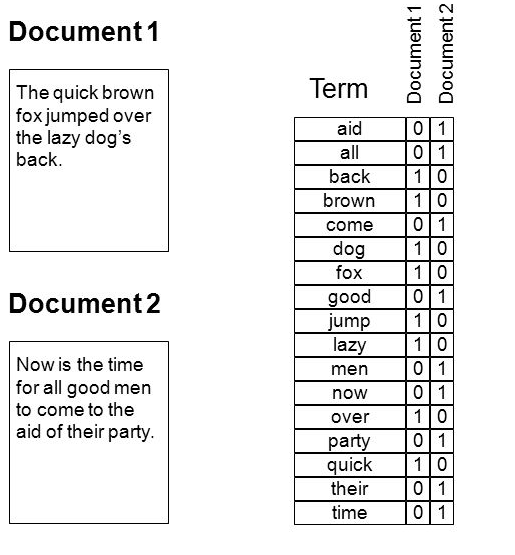
\includegraphics[height=10cm]{bag_of_words.png}
  \captionof{figure}{Пример мешков для двух предложений\cite{Goodfellow-et-al-2016}}\label{fig:domain:bag_of_words}
\end{center}

Для классификации предложений выделение особенностей начинают со статической обработки текста, например убирают символы переноса строки, или заменяют символы, которые могут использоваться в формате представления набора данных, на аналоги или ключевые слова. Часто используется замена символов круглых скобок на сокращения «--LRB--» и «--RRB--». С этим легко справится механизм регулярных выражений. Затем необходимо разбить предложения на единицы языка, несущие независимое семантическое значение --- произвести токенизацию. Для большинства языков регулярные выражения так же справятся с задачей. Для русского языка хватит разбиения по символу пробела, в английском надо будет учитывать еще и апострофы («It's» разобьется на «It» и «'s»). Однако для обработки большинства восточных языков так же приходится прибегать к машинному обучению, так как синтаксическое разделение слов на письме часто отсутствует, и токенизацию можно произвести только анализируя семантическое значение предложения. Для ограничения масштаба в данной работе методы токенизации рассматриваться не будут\cite{Goodfellow-et-al-2016}.
В работе для токенизации и синтаксического разбора будут использованы средства CoreNLP встроенные в библиотеку NLTK для Python.

Итак, после токенизации предложения представляют из себя набор единиц языка в строковом формате. Но нейронные сети работают только с числами. Поэтому необходимо представить слова в векторном виде. Данный процесс называется \textit{встраивание слов}. Классический метод \en{one-hot-encoding} заключается в представлении слова в виде позиционных кодов. Для всех уникальных слов в корпусе строится словарь, где каждому слову соответствует вектор заполненный нулями и одной единицей, соответствующей позиции слова в словаре. Очевидно, это очень производительный метод встраивания слов, так как алгоритм кодирования слов в новом корпусе имеет линейную сложность. Однако прямая зависимость размера вектора от количества уникальных слов в корпусе может вызвать проблемы с хранением этих векторов. Например, корпус книг от Google содержит 1 миллион уникальных слов, и с one-hot-encoding каждое слово будет занимать 30 мегабайт памяти, если пользоваться в вычислениях хотя бы 32-битными числами. Так же семантическое значение слов в данном методе теряется --- сравнение синонимов, антонимов и никак не связанных между собой по значению слов даст один и тот же результат. Метод сжатия векторов слов в единый вектор, соответствующий предложению, заключается в простом суммировании векторов слов и носит название \textit{Мешок слов}.\cite{Goodfellow-et-al-2016}. Пример представлен на рисунке~\ref{fig:domain:bag_of_words}.

Скалярное произведение двух таких векторов предложений даст степень схожести этих предложений, основывающейся только на количестве одинаковых слов встречающихся в обоих предложениях. Таким образом данный метод для трех предложений «Мальчик ударил мяч.», «Мальчик ударился в учебу» и «Дети играют в футбол» сделает вывод о том, что схожи первые два предложения, хотя очевидно что по смыслу больше связаны первое и третье. Обучение нейронной сети на выборке из мешков слов не даст никаких результатов для задач классификации по значению не только по причине отсутствия семантики в векторных представлениях слов и фраз, но и из-за представления в виде позиционных кодов, когда большая часть вектора не несет никакой нагрузки, а содержит лишь ноли\cite{Goodfellow-et-al-2016}.
\subsection{Технология word2vec}\label{subsec:domain:domain_word2vec}
Существует ряд методов встраивания слов, в которых векторы сохраняют семантическое значение обрабатываемых слов. В основе этих техник лежит идея о том, что семантика слова заключена в контексте его применения. Самым значимым результатом исследований на почве этой идеи является технология word2vec. На сегодняшний день это самый распространенный и эффективный метод встраивания слов. Качественно обученная модель word2vec представляет собой словарь, в котором словам соответствуют так называемые плотные вектора\cite{word2vec}.

Процесс обучения модели word2vec начинается с генерации произвольных значений векторов для изучаемых слов. Каждому слову будет соответствует два плотных вектора, так как слово в процессе обучения может участвовать в роли центрального слова, и в роли слова из контекста центрального слова. На каждом шаге обучения в тексте последовательно выбирается центральное слово и его контекст --- слова которые отстоят от центрального на m слов слева и справа. Для каждого центрального слова t делается предсказание слов в контексте\cite{word2vec}. Целевой функцией оптимизации в данном случае будет
\begin{gather}
  J^{\prime}(\Theta) = \prod_{t=1}^{T}\prod_{\substack{-m\leq j \geq m\\j \neq 0}}p(w_{t+j}|w_{t};\Theta),
\end{gather}
\begin{explanationx}
\item [где] $ \Theta $ --- это параметры модели, изменяемые в ходе обучения.
\end{explanationx}

Тогда отрицательная логарифмическая функция максимального правдоподобия $ J(\Theta) $ будет равна:
\begin{gather}
  \label{eq:domain:word2vec:J}
  J(\Theta) = -\frac{1}{T}\sum_{t=1}^{T}\sum_{\substack{-m\leq j \geq m\\j \neq 0}}\log(p(w_{t+j}|w_{t})).
\end{gather}
Для предсказания вероятности слова в контексте применяется функция \en{softmax}, описанная в общем виде в выражении
\begin{gather}
  \label{eq:domain:softmax}
  {\sigma(z)}_i = \frac{e^{z_i}}{\sum_{k=1}^{K}e^{z_k}}.
\end{gather}
Вероятность нахождения слова $o$ в контексте слова $c$ --- это softmax функция для $c$ по $o$
\begin{gather}\label{eq:domain:word2vec:contex_prob}
  p(o|c) = \frac{\exp({u_{o}^T}\cdot{v_{c}})}{\sum_{w=1}^{V}\exp({u_w^T}\cdot{v_{c}})}.
\end{gather}
Матрица $U$ хранит вектора в для слов из контекста, а $V$ --- для центральных слов.
Градиент для обратного прохода для~\ref{eq:domain:word2vec:J} и~\ref{eq:domain:word2vec:contex_prob} будет равен:
\begin{gather}
  \frac{\partial }{\partial v_c}\frac{\exp({u_{o}^T}\cdot{v_{c}})}{\sum_{w=1}^{V}\exp({u_w^T}\cdot{v_{c}})} = u_o - \sum_{x=1}^{V}p(x|c)\cdot{u_x}.
\end{gather}
После того, как градиент рассчитан значение градиента отнимается от всех обучаемых параметров модели, то есть от матриц $U$ и $V$.

В результате множества итераций обучения будет получена простейшая softmax модель word2vec, которая будет представлять из себя матрицу $V$. Полученные вектора хранят семантическое значение слов, таким образом близкие по смыслу слова и синонимы будут располагаться близко друг от друга. А математические операции над этими векторами будут давать интересные результаты. Например если отнять от вектора «Король» вектор «Мужчина» и добавить вектор «Женщина» то будет получен вектор слова «Королева». На рисунке~\ref{fig:domain:word2vec} видно, что вектора располагаются параллельно вдоль некоторых осей, выученных моделью, по признакам пола, части речи и географического положения. Реализовать статическую модель распознающую подобные признаки невероятно трудно\cite{word2vec}.
\begin{center}
  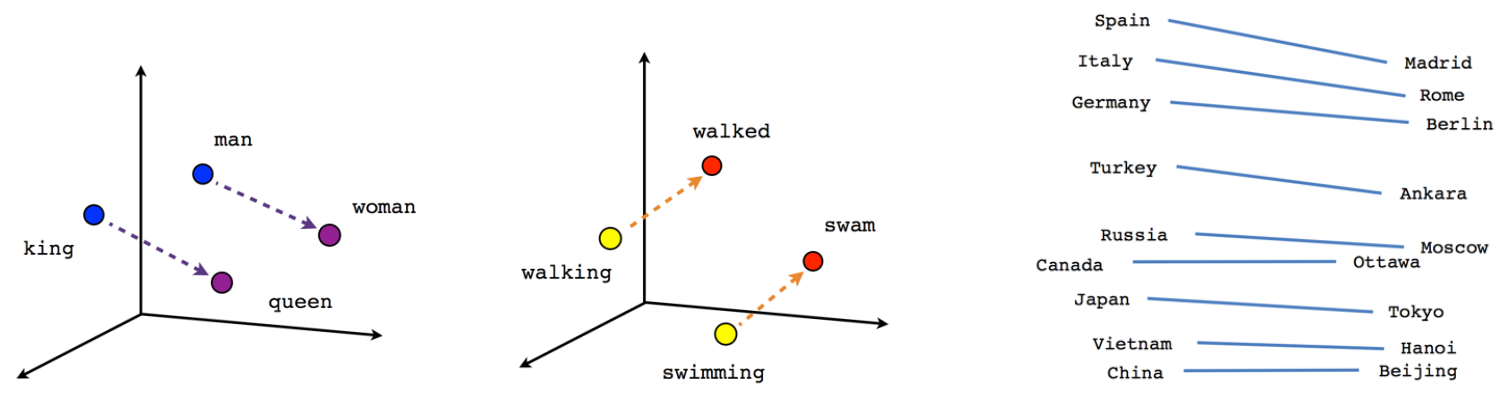
\includegraphics[height=4cm]{word2vec.png}
  \captionof{figure}{Отношение между векторами в примере word2vec\cite{word2vec}}\label{fig:domain:word2vec}
\end{center}
\subsection{Классическая рекурсивная нейронная сеть}\label{subsec:domain:rnn}
Когда каждое предложение представляет собой набор векторов, соответствующих языковым единицам, необходимо провести сжатие --- обработать вектора слов таким образом, чтобы каждому предложению соответствовал один плотный вектор. Простейшая нейронная сеть, которая может быть применена в данной задаче --- это рекурсивная нейронная сеть (RNN). Данная сеть имеет два входа: $x_{t}$ --- входной вектор, $s_{t-1}$ --- вектор состояния с прошлой итерации. Сеть последовательно применяется к векторам в предложении слева направо, и выдает на каждой итерации выходной вектор $o_{t}$ и вектор состояния $s_t$.

Состоит сеть из трех матриц весов: входная матрица $U$, матрица состояний $W$, матрица выходов $V$. B описывается двумя функциями~\ref{eq:domain:rnn:state} и~\ref{eq:domain:rnn:output}. Softmax функция описана в~\ref{eq:domain:softmax}. Пример рекурсивной нейронной сети и ее развертки во времени представлен на рисунке~\ref{fig:domain:rnn}.
\begin{gather}
  \label{eq:domain:rnn:state}
  s_t = f(U\cdot{x_t} + W\cdot{s_{t-1}}),\\
  \label{eq:domain:rnn:output}
  o_t = softmax(Vs_t),
  \end{gather}
\begin{explanationx}
\item [где] $f$ --- это функция активации, обычно выбирают тангенс.
\end{explanationx}

После обхода всего предложения, получается выходной вектор, и появляется возможность посчитать функцию потерь, и вычислить значение градиента. На рисунке~{fig:domain:rnn} показана развертка во рекурсивной сети во времени. Таким образом модель можно представить в виде многослойной сети. А значит модель страдает от проблемы затухающего градиента, когда градиентный спуск необходимо произвести на множество слоев вниз, и значение функции ошибки может очень сильно отличаться от реального ее значения. Но так как применяется одна и та же сеть на каждом слое, то проблема затухающего градиента для рекурсивной сети усиливается. Поэтому с помощью RNN не было получено высоких результатов в классификации предложений.

\begin{center}
  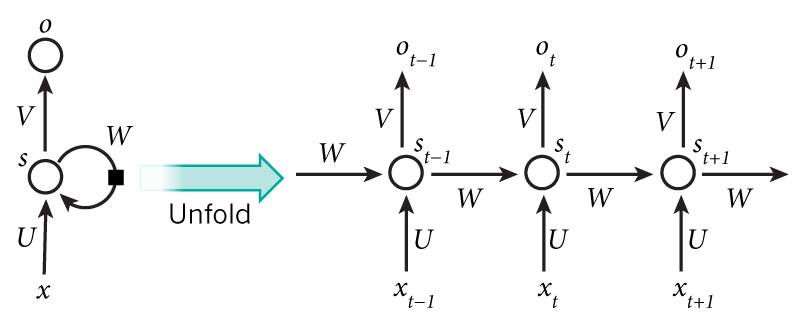
\includegraphics[height=4cm]{rnn.png}
  \captionof{figure}{Рекурсивная нейронная сеть в развертке во времени\cite{Goodfellow-et-al-2016}}\label{fig:domain:rnn}
\end{center}

Так же рекурсивная сеть сталкивается с проблемой отдаленных зависимостей. Суть проблемы в том, что семантически связанные слова, которые имеют главную роль в понимании предложения, могут находиться удаленно друг от друга в предложении. И так как RNN обходит предложение слева на право, то информация о том, что первое слово встречалось в предложении может уже быть потеряно к тому моменту, как на вход придет второе, и модель сделает неверный вывод.

\subsection{Long Short Term Memory}\label{sec:domain:lstm}
Проблему отдаленных зависимостей решает нейронная сеть под названием Long Short Term Memory (LSTM). Это особый вид рекурсивной нейронной сети, способная выучить удаленные зависимости. Данное свойство было получено за счет усложнения структуры сети. Принцип применения и обучения остался таким же: предложение обходится слева направо последовательно подавая на вход сети плотные вектора соответствующие словам. Схема сети представлена на рисунке~\ref{fig:domain:lstm}.

Внутреннее состояние сети описывается вектором состояния ячейки $C_t$ и вектором скрытого слоя $h_t$. На вход принимает входной вектор $x_t$ и состояние с прошлой итерации: $C_{t-1}$ и $h_{t-1}$. Выходной вектор $o_t$ равен вектору скрытого слоя $h_t$. Введена система врат. Врата блокируют или пропускают векторы между различными состояниями нейронной сети. $f_{t}$ --- сигнал забывания, сбрасывает состояния ячейки. $i_{t}$ --- входные врата, блокируют или пропускают входной вектор. И $o_t$ --- выходные врата, блокируют или пропускают выходной вектор\cite{LSTM}.

\begin{center}
  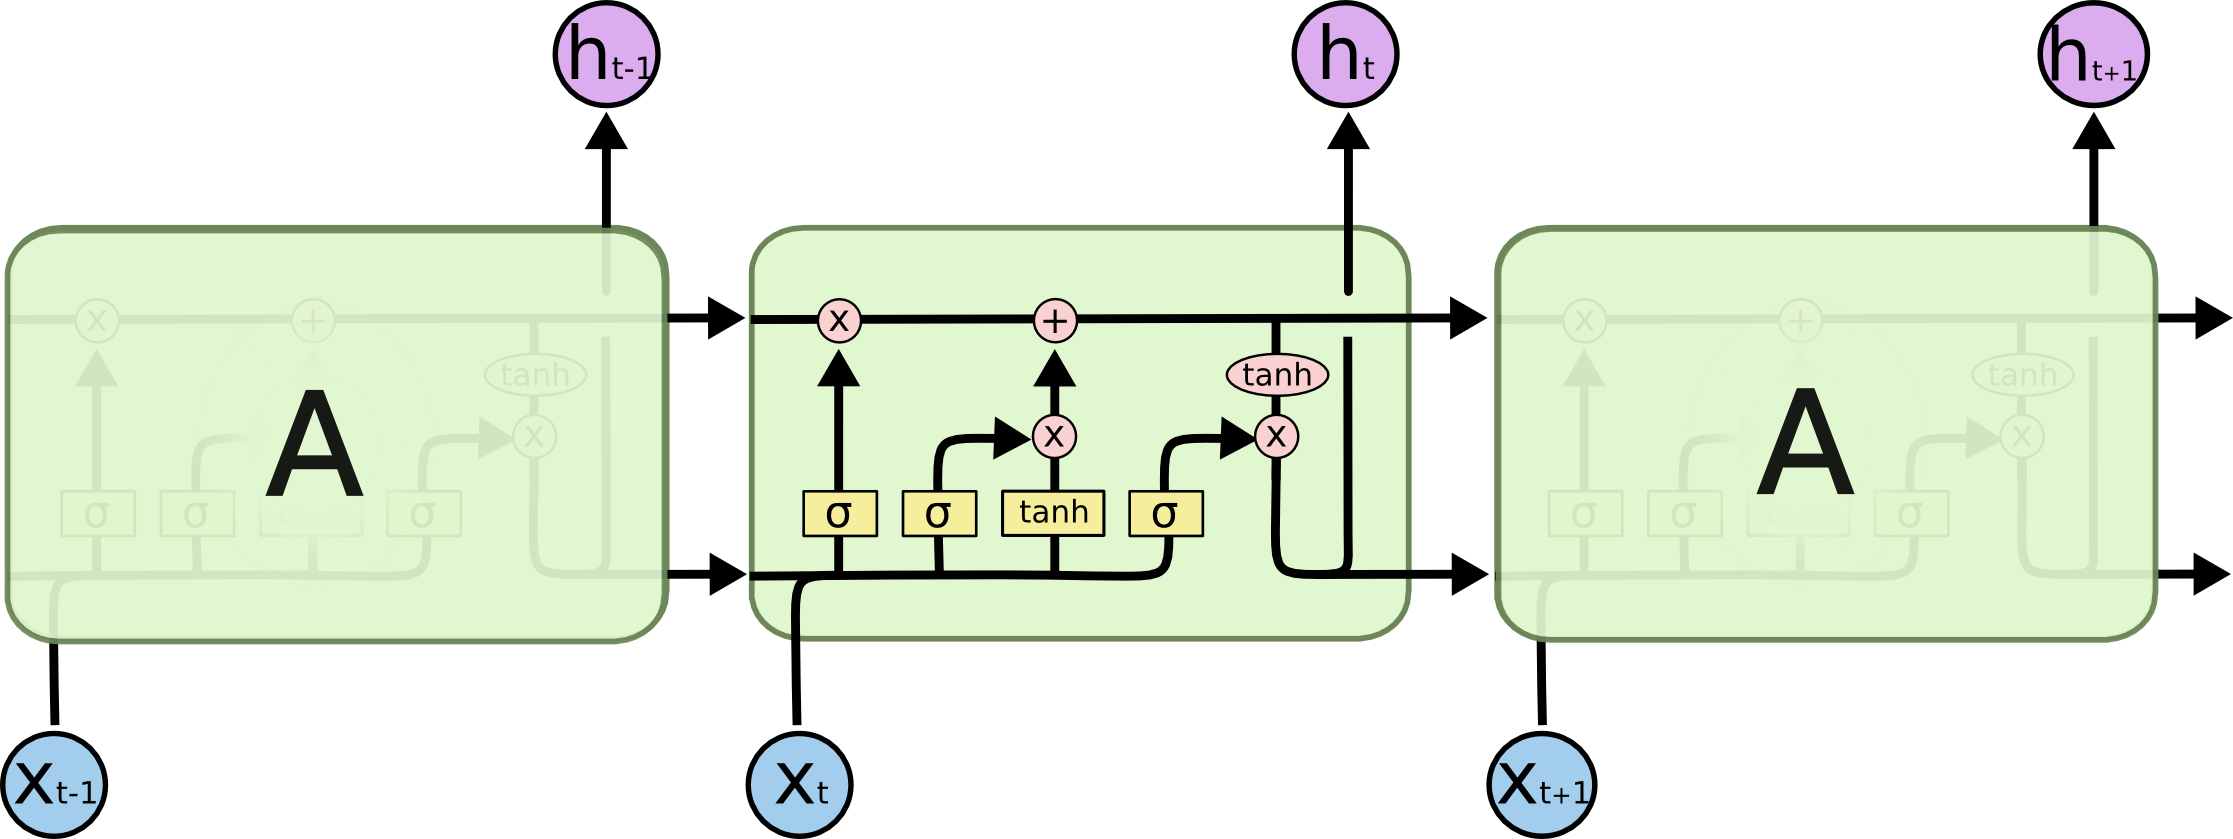
\includegraphics[height=4cm]{lstm.png}
  \captionof{figure}{Схематическое изображение LSTM-сети\cite{LSTM}}\label{fig:domain:lstm}
\end{center}

Состояния врат описаны выражениями~\ref{eq:domain:lstm:input_gate},~\ref{eq:domain:lstm:output_gate} и~\ref{eq:domain:lstm:forget_signal}.
\begin{gather}
  \label{eq:domain:sigmoid}
  \sigma(x) = \frac{1}{1 + e^{-x}},\\
  \label{eq:domain:lstm:input_gate}
  i_t = \sigma(W_{i}\cdot{x_t} + U_{i}\cdot{h_{t-1}} + b_i),\\
  \label{eq:domain:lstm:forget_signal}
  f_t = \sigma(W_{f}\cdot{x_t} + U_{f}\cdot{h_{t-1}} + b_f),\\
  \label{eq:domain:lstm:output_gate}
  o_t = \sigma(W_{o}\cdot{x_t} + U_{o}\cdot{h_{t-1}} + b_o),
\end{gather}
\begin{explanationx}
\item [где] $\sigma$ это функция сигмоида описанная~\ref{eq:domain:sigmoid};
\item $W$ и $U$ --- это тензоры весов LSTM\@.
\end{explanationx}

Состояния ячейки вычисляются согласно выражениям~\ref{eq:domain:lstm:cell_candidate},~\ref{eq:domain:lstm:new_cell} и~\ref{eq:domain:lstm:new_hidden}.
\begin{gather}
  \label{eq:domain:hadamar}
  {(A\odot{B})}_{i,j} = {(A)}_{i,j}\cdot{{(B)}_{i,j}},\\
  \label{eq:domain:lstm:cell_candidate}
  \tilde{C}_t = \tan(W_{C}\cdot{x_{t}} + U_{c}\cdot{h_{t-1}} + b_c),\\
  \label{eq:domain:lstm:new_cell}
  C_t = f_t\odot{c_{t-1}} + i_t\odot{\tilde{C}_t},\\
  \label{eq:domain:lstm:new_hidden}
  h_t = o_t\odot{\tan(c_t)},
\end{gather}
\begin{explanationx}
\item [где] $\tilde{C}_t$ носит название кандидата в состояние ячейки;
\item ${\odot}$ --- это операция произведения Адамара, описанная в~\ref{eq:domain:hadamar} для двух матриц $A$ и $B$.
\end{explanationx}

Архитектура Multiple LSTM, один из вариантов LSTM, на сегодняшний день лежит в основе самой эффективной модели анализа тональности предложений Sentiment Neuron от сообщества OpenAi. Помимо лидерства на текущий момент, Sentiment Neuron обучается без учителя --- это единственная успешная модель способная сжимать вектора слов в плотный вектор предложения и обучающая без учителя. Однако обучение этой модели крайне дорого. OpenAi обучали ее на четырех Nvidia Pascal Titan X и обучение заняло приблизительно один месяц\cite{openai}.

\subsection{Рекурсивная тензорная нейронная сеть}
Проблема отложенных связей может решаться иначе. Очевидно, что порядок слов в предложении редко совпадает с нитью размышлений автора. Обход предложения слева направо не может запомнить все семантически значимые последовательности, особенно в языках со специфической грамматикой. Поэтому исследователи решили изменить порядок обхода предложений. Один из итогов исследований --- это модель рекурсивной нейронной тензорной сети (RNTN), которая легла в основу CoreNLP\@. Обход предложения производится по синтаксическому дереву, построенному согласно генеративной грамматике Хомского\cite{Chomsky}.
Итак, в процесс выделения особенностей добавляется еще один шаг --- синтаксический анализ предложения. Для RNTN необходимо на входе иметь синтаксическое дерево составляющих --- один из видов синтаксических деревьев. Это дерево удобно тем, что его можно нормализовать, то есть привести к виду бинарного дерева. На рисунке~\ref{fig:domain:constituency_tree} показан пример синтаксического дерева составляющих\cite{Chomsky}.

\begin{center}
  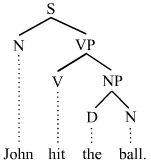
\includegraphics[height=5cm]{constituency_tree.png}
  \captionof{figure}{Пример синтаксического дерева составляющих\cite{wiki:dep_grammar}}\label{fig:domain:constituency_tree}
\end{center}

Как видно из рисунка~\ref{fig:domain:constituency_tree}, слова представлены листьями дерева, а его узлы --- это различные виды составляющий в предложении. Типы связей не нужны в модели RNTN, интересен только сам факт их наличия и какие слова и фразы они объединяют. Для того, чтобы эффективно обрабатывать дерево составляющих, RNTN модифицирована и имеет два входа, и один выход. То есть она принимает два вектора с нижних узлов и передает верхнему, и т.д., пока в результате обработки всего дерева не будет получен один вектор, соответствующий всему предложению. Так же модель выдает вектор для каждого узла в дереве, что соответствует фразам в предложении. Это свойство эффективно применяется при обучении. Специально для обучения RNTN был создан Stanford Sentiment Treebank (SST) --- Стенфордский набор деревьев тональности. Это набор более чем из десяти тысяч синтаксических деревьев, все узлы которых оценены по тональности носителями языка. SST стал очень популярен и вне исследований RNTN и является классическим набором для измерения эффективности метода оценки тональности\cite{RNTN}.

Пусть $\begin{bmatrix}a\\b\end{bmatrix}$ --- два вектора размерности $d$ объединенные в один размерностью $2d$. Тогда значение вектора результата $p$ для входных векторов $a$ и $b$ высчитывается по формуле~\ref{eq:domain:rntn:p}\cite{RNTN}.
\begin{gather}
  \label{eq:domain:rntn:p}
  p = f(
  \begin{bmatrix}
    a\\
    b
  \end{bmatrix}^{T}\cdot{V}\cdot{
  \begin{bmatrix}
    a\\
    b
  \end{bmatrix}} + W\cdot{
  \begin{bmatrix}
    a\\
    b
  \end{bmatrix}}),
\end{gather}
\begin{explanationx}
\item [где] $f$ --- функция активации;
\item $V$, $W$ --- матрицы весов модели.
\end{explanationx}

\subsection{Tree LSTM}
На следующий год после релиза RNTN, изменяется подход в синтаксическом разборе предложений, так как выходит работа с описанием алгоритма синтаксического разбора с линейной сложностью. Однако этот алгоритм возвращает дерево зависимостей, а RNTN работает с деревом составляющих. Пример дерева зависимостей представлен на рисунке~\ref{fig:domain:dependency_tree}. Дерево зависимостей несет в себе меньше информации, чем дерево составляющих, так как дерево составляющих можно сконвертировать в зависимости без потерь, а обратный процесс без потерь невозможен\cite{Chomsky}.

\begin{center}
  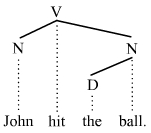
\includegraphics[height=5cm]{dependency_tree.png}
  \captionof{figure}{Пример синтаксического дерева зависимостей\cite{wiki:dep_grammar}}\label{fig:domain:dependency_tree}
\end{center}

Дерево зависимостей для задачи классификации отличается тем, что каждый узел дерева содержит вектор слова. Так же дерево не является бинарным --- каждый узел может иметь произвольное количество детей.

Для обработки подобных деревьев была разработана модель Tree LSTM, которая существует в двух модификациях: $N$-арная Tree LSTM, для деревьев составляющих и Child-Sum Tree LSTM, для работы с деревьями зависимостей. В данной работе была реализована модель Child-Sum Tree LSTM\cite{tree_lstm}.

Итак, ячейка Child-Sum Tree LSTM в некотором узле дерева принимает на вход состояния дочерних узлов. Пример подключения показан на рисунке~\ref{fig:domain:tree_lstm}.

Состояние ячейки Tree LSTM, как и в обычной LSTM, описано двумя векторами: $h_j$ и $c_j$ --- значение скрытого слоя и внутреннего состояния соответственно. Состояние для узла $j$, имеющего множество детей $C(j)$ можно выразить следующим образом:
\begin{gather}
  \tilde{h_j} = \sum_{k\in{C(j)}}h_k,\\
  \label{eq:domain:tree_lstm:i}
  i_j = \sigma(W^{(i)}\cdot{x_j} + U^{(i)}\cdot{\tilde{h_j}} + b^{(i)}),\\
  \label{eq:domain:tree_lstm:forget}
  f_{jk} = \sigma(W^{(f)}\cdot{x_j} + U^{(f)}\cdot{h_k} + b^{(f)}),\\
  \label{eq:domain:tree_lstm:o}
  o_j = \sigma(W^{(o)}\cdot{x_j} + U^{(o)}\cdot{\tilde{h_j}} + b^{(o)}),\\
  \label{eq:domain:tree_lstm:u}
  u_j = \tan(W^{(u)}\cdot{x_j} + U^{(u)}\cdot{\tilde{h_j}} + b^{(u)}),\\
  c_j = i_j\odot{u_j} + \sum_{k\in{C(j)}}f_{jk}\odot{c_k},\\
  h_j = o_j\odot{\tan(c_j)},
\end{gather}
\begin{explanationx}
\item [где] $k\in{C(j)}$ для выражения~\ref{eq:domain:tree_lstm:forget}.
\end{explanationx}

В результате обработки всего дерева будет получен плотный вектор предложения.

\begin{center}
  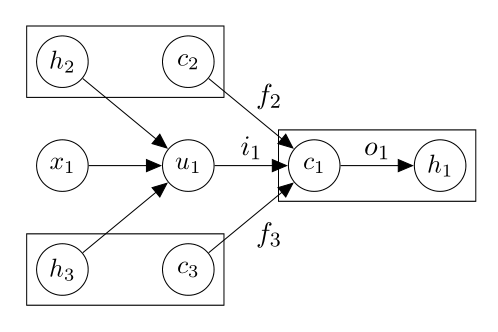
\includegraphics[height=6cm]{tree-lstm.png}
  \captionof{figure}{Пример подключения узла Tree LSTM к дочерним узлам. $h_2$, $c_2$, $h_3$, $c_3$ --- состояния двух дочерних узлов, $h_1$, $c_1$ --- состояние узла родителя. $x_1$ --- входной вектор узла.\cite{tree_lstm}}\label{fig:domain:tree_lstm}
\end{center}

\subsection{Классификация}
Последним этапом NLP-конвейера будет классификация плотных векторов предложений, полученных в результате сжатия. Стоит отметить, что плотные вектора предложений кодируют различные семантические свойства этих предложений, а значит с их помощью можно решать различные задачи классификации. Например сравнивать предложения по значению, похожи ли они, или противоположны, либо же нейтральны. Однако в данной работе интересная задача оценки тональности текста\cite{Goodfellow-et-al-2016}.

Для оценки тональности обычно обучают простейшую регрессионную модель
\begin{gather}
  p_{\Theta}(y|x_j) = softmax(W\cdot{h_j} + b),\\
  y_j = \arg \max_y(p_{\Theta}(y|x_j)),
\end{gather}
\begin{explanationx}
\item[где] $h_j$ --- это плотный вектор предложения;
\item$\arg \max_y$ --- функция, которая вернет индекс максимального элемента вектора.
\end{explanationx}

Задача регрессионной модели в том, чтобы построить линию регрессии таким образом, чтобы средний квадрат расстояний от линии регресси до элементов популяции был наименьшим. На рисунке~\ref{fig:domain:dense_population} показан пример линии регресси в плотной популяции. Как видно из ресунка, не существует способа провести линию так, чтобы расстояние от линии до всех элементов популяции было равно нулю. То есть, регрессионная модель имеет предел точности, до которой ее можно обучить, и носит название неустранимой ошибки.

\begin{center}
  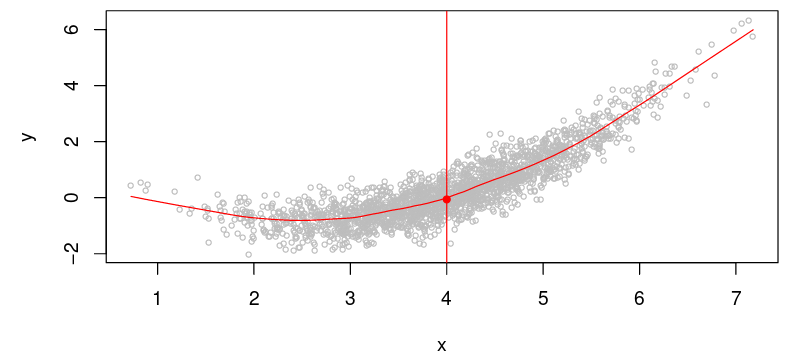
\includegraphics[height=6cm]{dense_population.png}
  \captionof{figure}{Пример линии регрессии для плотной выборки\cite{stanford_course}}\label{fig:domain:dense_population}
\end{center}

Таким образом, ошибка системы делится на устранимую и неустранимую ошибки. Классический подход в обучении нейронной сети заключается в том, чтобы разбить тренировочный набор данных на три части:
\begin{itemize}
\item train --- тренировочная часть;
\item dev или hold out --- отложенная часть;
\item test --- проверочная часть.
\end{itemize}

Тренировочная часть обущающего набора данных применяется непосредственно для обучения модели. Проверочная часть используется для проверки обученной модели на неизвестых модели данных. На рисунке~\ref{fig:domain:train_vs_test} показан пример того, как изменяется точность модели в зависимости от гибкости. Под гибкостью модели понимается ее линейность. Чем больше компонент в уравнении линии регрессии, тем больее сложные фигуры сможет описывать линия на графике, и тем меньше будет средний квадрат расстояний до элементов выборки. Верхний график на рисунке соответствует ошибке на проверочной части обучающего набора данных, нижний график --- ошибка на тренировочной части. Пнктирная линия --- это теоретический попрог точности модели, то есть неустранимая ошибка. Как видно из рисунка, наиболее гибкая модель хорошо подстраивается под тренировочную часть, но на проверочной части показывает себя еще хуже, чем линейная модель. Данный феномен носит название переобучения модели.

\begin{center}
  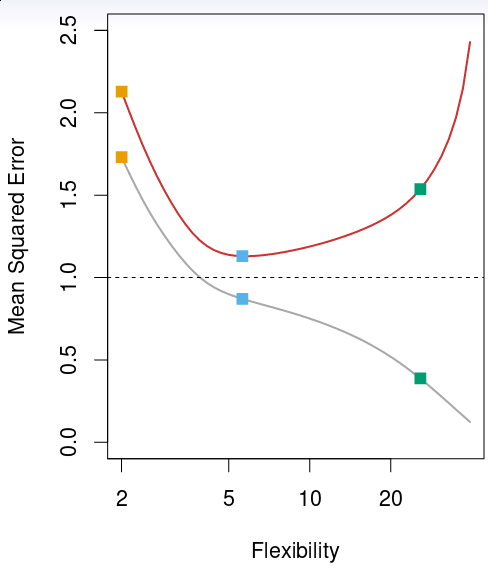
\includegraphics[height=12cm]{train_vs_test.png}
  \captionof{figure}{Зависимость точности модели от ее гибкости\cite{stanford_course}}\label{fig:domain:train_vs_test}
\end{center}

Для борьбы с переобучением применяется регуляризация. Для этого функция ошибки модели разбивается на три части следующим образом:
\begin{gather}
  Y = f(X) + \epsilon,\\
  f(x) = E(Y|X=x),\\
  \label{eq:domain:bias_var_tradeoff}
  E{(y_0-\tilde{f}(x_0))}^2 = Var(\tilde{f}(x_0)) + {[Bias(\tilde{f}(x_0))]}^2 + Var(\epsilon),
\end{gather}
\begin{explanationx}
\item[где] $f$ --- это идеальная модель;
\item $\epsilon$ --- неустранимая ошибка;
\item $E$ --- функция ошибки;
\item $Var$ --- дисперсия;
\item $Bias$ --- смещение;
\item $x_0, y_0$ --- элементы выбоки;
\item $\tilde{f}$ --- обучаемая модель.
\end{explanationx}

Как видно из выражения~\ref{eq:domain:bias_var_tradeoff}, ошибка разбивается на три части:
\begin{itemize}
\item дисперсия предсказателя;
\item отклонение предсказателя;
\item неустранимая ошибка.
\end{itemize}

Дисперсия предсказателя выражает то, насколько сильно разбрасываются значения предсказаий для одних и тех же входных данных, при обучении модели на разных наборах данных. Соотетственно, данная компонента ошибки модели будет выше для более гибких моделей, так как значения предсказаний более зависимы от тренировочной выборки, чем для линейной модели.

Смещение предсказания выражает то, насколько высоко смещение предсказаний модели от значений в популяции. Соответственно для более гибкой модели это значение будет ниже, чем для менее гибкой, так как она больше подстраивается под выборку и дает более точные предсказания, если не было достигнуто переобучение модели. На рисунке~\ref{fig:domain:traidoff} показаны графики для среднеквадратической ошибки вверху, ниже графики дисперсии, и внизу графики отклонения, для разных наборов данных. Как видно из рисунка, большое влияние на то, какой гибкости модель подойдет для решения задачи, оказывает структура набора данных. Поэтому для каждой задачи должна производится отдельная настройка модели, для чего используется отложенная часть обучающего набора данных.

\begin{center}
  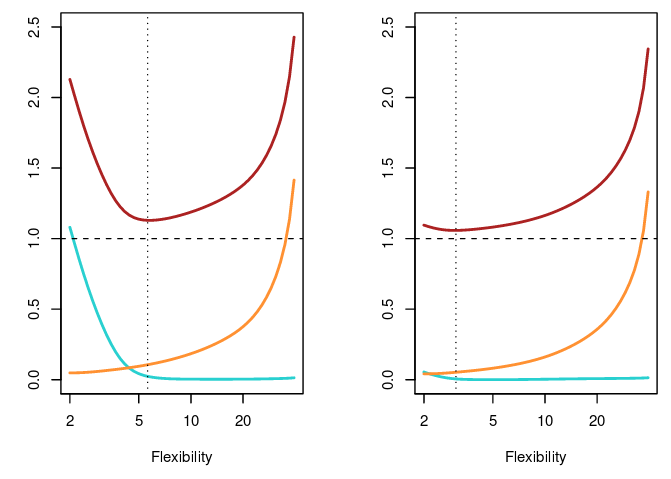
\includegraphics[height=8cm]{traidoff.png}
  \captionof{figure}{Зависимость различных компонент ошибки от гибкости модели для двух наборов данных\cite{stanford_course}}\label{fig:domain:traidoff}
\end{center}

Итак, для того, чтобы управлять компонентами ошибки, применяется регуляризация линейной регрессии. В данной работе применялась регуляризация L2, при которой регрессия выражается следующим образом:
\begin{gather}
  p_{\Theta}(y|x_j) = softmax(W\cdot{h_j} + b + \lambda\cdot{R(W)}),\\
  R(W) = frac{1}{2}\cdot{W^T}\cdot{W},
\end{gather}
\begin{explanationx}
\item[где] $\lambda$ --- коэффициен регуляризацииб является гиперпараметром модели.
\end{explanationx}

Пример работы регуляризации показан на рисунке~\ref{fig:domain:regularization}. С помощью L2 регуляризации увеличивают смещение модели, то есть точечные предсказания будут имень большее расстояние до идеальных значений, но за счет уменьшени значения модель станет более стабильной и проблема переобучения наблюдаться не будет.

\begin{center}
  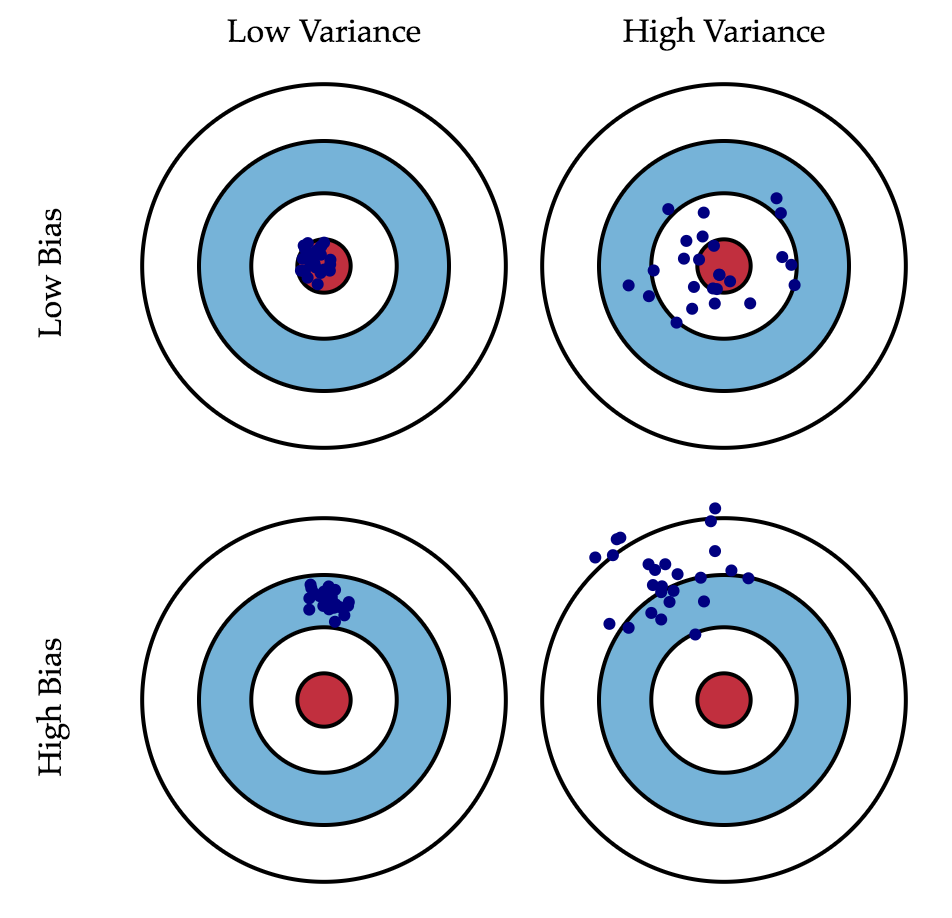
\includegraphics[height=8cm]{regularization.png}
  \captionof{figure}{Изменения дисперсии и смещения при регуляризации\cite{stanford_course}}\label{fig:domain:regularization}
\end{center}

% \section{СИСТЕМНОЕ ПРОЕКТИРОВАНИЕ}\label{sec:sys}
Изучив теоретические аспекты разрабатываемого приложения и выработав список требований необходимых для разработки модуля, разбиваем систему на компоненты.
В разрабатываемом приложении можно выделить следующие блоки:
\begin{itemize}
\item модуль сбора статистики;
\item модуль объектно-реляционного отображения;
\item база данных объектов для анализа;
\item модуль развертки;
\item тренировочный набор Стенфорда;
\item модуль выделения особенностей;
\item модуль модели анализатора;
\item модуль ячейки Tree LSTM\@;
\item визуализации CoreNLP\@;
\item модуль визуализации TensorBoard.
\end{itemize}
Структурная схема, иллюстрирующая перечисленные блоки и связи между ними приведена на чертеже ГУИР.400201.009 C1.


\subsection{Подготовка данных}\label{subsec:sys:data_gathering}
Чтобы начать работу модели распознавания тональностей, необходимы входные данные. Первый тип входных данных --- это тренировочный набор Стенфорда. Он необходим для обучения модели распознаванию тональностей. Стенфордский набор Представляет собой выборку синтаксических деревьев составляющих. Однако модель должна работать с синтаксическими деревьями зависимостей. Поэтому необходимо привести его к виду синтаксических деревьев зависимостей. Так как исследование синтаксического разбора не входит в задачи проектирования, то для этой цели будет использоваться синтаксический анализатор из CoreNLP\@. Он не является самым производительным, но самым простым в применении. За несколько секунд он обрабатывает более 10000 предложений, составляющих Стенфордский тренировочный набор. Обработать тренировочный набор необходимо всего один, при установке программы, поэтому скорость в несколько секунд вполне удовлетворительна. Объем анализатора вместе с моделью нейросети, обученной синтаксическому разбору, составляет более 350 мегабайт. Далее нужен предобученный набор встроенных векторов GloVe\@. Он содержит в себе 5 гигабайт слов и соответствующих им векторам размерностью в 300 составляющих каждый. Чтобы сократить размер, занимаемый набором GloVe\@, он будет отфильтрован: будут выброшены все слова, которые не встречаются в Стенфордском тренировочном наборе. После такой фильтрации набор встраиваемых векторов будет занимать около 30 мегабайт дискового пространства. Фильтрацию так же необходимо произвести только один раз при установке программы. То есть, если перед началом работы программы произвести предобработку входных данных, то это повысит производительность и сократить объем, занимаемый системой на диске. Итак, чтобы решать проблему управления зависимостями, введен модуль развертки. В его задачи входит:

\begin{itemize}
\item проверить наличие отфильтрованного набора GloVe;
\item проверить наличие тренировочного набора в виде синтаксических деревьев зависимости;
\item проверить наличие синтаксического анализатора и скачать его, если отсутствует;
\item при необходимости скачать оригинальные набор GloVe и тренировочный набор;
\item при необходимости отфильтровать GloVe и удалить оригинальную версию;
\item при необходимости обработать оригинальный Стенфордский тренировочный набор с помощью синтаксического анализатора;
\item проверить наличием необходимых библиотек и установить отсутствующие.
\end{itemize}

В результате работы модуля развертки, модель будет способна обучаться. Для того чтобы расширить возможности исследования возможностей модели, введен модуль сбора статистики. Его задачей будет сбор данных с сайта rottentomatoes.com, популярного форума о кино. Там собрано множество отзывов о фильмах последних десятилетий. Так же он предоставляет API для разработчиков, что поможет в сборе данных с ресурса. Для демонстрации хватит отзывов профессиональных критиков и обычных пользователей, и рейтинга фильма. Собранные через API данные необходимо хранить в базе данных, так как сбор данных для анализа может занять значительно больше времени, чем сам анализ. А база данных поможет сохранить результаты, и продолжить сбор информации в любое удобное время.

Так как сбор данных через API --- задача достаточно тривиальная, в которой производительность зависит от скорости обмена данными с сервером, то производительность языка Python даст удовлетворительные результаты. Так же Python скриптовый язык, что упростит разработку. Для работы с REST API отлично подойдет библиотека requests для Python, которая просто представят собой реализацию REST-интереса и довольно проста в использовании.

В качестве базы данных будет использована MySQL, как стабильное и надежное решение. Для удобства работа с базой данных будет организована по принципу объектно-реляционного отображения. Данный принцип предполагает абстракцию модели транзакций и предлагает программную модель --- объекты базы данных представляются в виде объектов в модели объектно-ориентированного программирования.

Для реализации объектно-реляционного отображения будет использована библиотека sqlalchemy, которая позволяет используя возможности языка Python максимально абстрагироваться от SQL\@. В объектах sqlalchemy будут хранится данные из базы данных. И любые изменения этих объектов sqlalchemy представляет в виде транзакции в базу, таким образом поддерживая актуальность данных в базе и в памяти программы.

Таким образом сбор данных для NLP-модели будет осуществляться модулем сбора статистики через API ресурса rottentomatoes.com. Полученные от сайта объекты REST будут сохраняться в объектах Python, которые в свою очередь, являясь объектом-реляционным отображениями базы данных, будут управлять данными в базе. И затем, когда данные из базы данных потребуется проанализировать, то они будут загружены в виде Python-объектов в рамках той же объектно-реляционной модели.

\subsection{Анализ данных}\label{subsec:sys:data_analysis}
В модели нейронной сети может протекать два процесса: обучение и анализ. Обучение сети выполняется с помощью тренировочного набора Стенфорда. А анализ происходит на обученной сети с данными, собранными модулем сбора статистики. Процесс обучения очень сложен в плане вычислений и требует много времени и ресурсов. Поэтому существует возможность сохранения обученной сети в файл и последующей загрузки из файла. Однако для исследовательских целей контроль обучения модели очень важен.

К тому же обучение модели Tree LSTM, за счет сложности архитектуры, происходит намного быстрее множества других нейронных сете. Процесс анализа же очень прост, так так математически нейронная сеть это линейная функция, и алгоритм анализа имеет линейную сложность.

Модуль выделения особенностей в процессе обучения модели выполняет синтаксический разбор тренировочного набора Стенфорда, что описано выше. В результате полученные деревья в виде списков Python сохраняются в формате JSON\@. В результате получается три набора: тренировочный, тестовый и набор разработки, каждый из которых составляет соответственно 10\%, 10\% и 80\% от всего набора Стенфорда. В процессе анализа данный модуль производит синтаксический разбор предложений, подлежащий обработке. И точно так же в JSON формате подается в модуль модели анализатора.

Модуль анализатора и модуль ячейки Tree LSTM представляют собой непосредственно саму нейронную сеть как математический алгоритм. В качестве основного инструмента реализации сети выбор пал на Tensorflow. В машинном обучении Tensorflow является стандартом на сегодняшний день. Данный фреймворк имеет API различных уровней абстракций: с использованием низкого уровня можно реализовывать модель в виде последовательности операций линейной алгебры, а на высоком уровне составными частями алгоритма являются слои нейронных сетей. Так же tensorflow предоставляет возможности выполнения вычислений на графических процессорах, и так же на тензорных процессорах (TPU).
Кроме того, tensorflow представил в конце 2017го технологию \textit{горячего выполнения}. Так как в классической архитектуре ПК оперативная память и память графического процессора разделены, и центральный процессор не имеет прямого доступа к видеопамяти, то программирование алгоритмов на графических процессорах вызывает сложности. Процесс написания кода на GPU с использованием популярных технологий, таких как CUDA, Torch, OpenCV и Tensorflow в том числе, заключается в предварительном построении графа выполнение, узлы которого --- это операции GPU, а грани --- это движение данных. И результат промежуточных вычислений недоступен, только выход всего графа целиком. Горячее вычисление предоставляет возможность получить промежуточные результаты без серьезных потерь производительности. Это во многом упрощает процесс отладки. В рамках данного проекта была построена модель с использованием этой техники. На данный момент в открытом доступе очень немного реализаций алгоритмов машинного обучения с горячими вычислениями.

Итак, модуль ячейки Tree LSTM представляет собой реализацию ячейки Child Sum Tree LSTM. Реализована она в виде класса наследника Model из модуля keras --- базового элемента высокоуровнего API keras. То есть, ячейка Tree LSTM является полноценным слоем в рамках tensorflow, и, что интересно в данной работе, поддерживает автоматический расчет градиента.

Модуль анализатора же не является классом keras, так как принимает на вход синтаксические деревья. Объекты tensorflow созданы для того, чтобы работать и на CPU и на GPU, поэтому обрабатывают они только тензоры, которые легко хранить в графической памяти. Дерево же довольно сложная структура, чтобы представить ее в виде тензора. Таким образом, модуль анализатора содержит в себе множество слоев нейронных сетей:

\begin{itemize}
\item слой проекции встроенных векторов;
\item слой исключения;
\item слой Child Sum Tree LSTM;
\item слой линейной регрессии.
\end{itemize}

Каждый узел синтаксического дерева будет проходить последовательно все эти слои в процессе обучения модели. В процессе выполнения слой регрессии будет выполнятся только в корне дерева.

Процесс анализа обученной моделью некоторого дерева начинается с подачи дерева на вход модели. Модель рекурсивно спускается к листьям дерева и выполняет последовательно слои модели на каждом узле. В результате работы на выходе линейной регрессии получается вектор, элементами которого являются вероятности принадлежности входного дерева каждому из целевых классов. Индекс элемента с наибольшей вероятностью и будет номером класса, в чью пользу модель сделала выбор.

Процесс обучения включает в себя многократное выполнение процесса анализа. Для обучения сети нужны тренировочный набор деревьев и набор разработки. Сам процесс обучения делится на эпохи. В ходе эпохи модель обрабатывает тренировочный набор целиком. В начале каждой эпохи элементы тренировочного набора перемешиваются в случайном порядке. Далее набор делится на равные группы, за исключением последней, если количество деревьев в наборе не кратно размеру группы. Каждая группа последовательно анализируется моделью, для каждого анализа по принципу обратной связи вычисляется функция потерь. Потери для деревьев в группе суммируются и после того, как группа целиком обработана, вычисляется градиент сети относительно каждого обучаемого параметра модели, куда в качестве аргумента передается суммарная потеря. Обучаемыми параметрами являются коэффициенты функций, которыми описаны различные слои нейронной сети. После этого, результаты градиента относительно каждого из обучаемых параметров сети добавляются к значениям этого же параметра.

После того, как обработаны все группы, эпоха считается законченной. Однако, кроме обучаемых параметров, модель имеет еще и гипер-параметры --- параметры, которые не возможно эффективно обучить методом градиентного спуска: например количество эпох, размер группы, количество элементов скрытого слоя того или иного слоя нейронной сети. Однако данные параметры играют очень важную роль в обучении сети и их успешный подбор зависит от опыта инженера. Для оценки успешности выбранных гипер-параметров, в конце каждой эпохи обучения производится анализ деревьев из набора разработки, и высчитывается оценка точности. Гипер-параметры изменяются для получения наилучшего результата точности на наборе разработки.

После того, как все эпохи обучения пройдены, модель анализирует деревья из тестового набора. Результирующая точность является качественной оценкой нейронной сети. Подбор гипер-параметров по тестовой выборке, вместо выборки разработки крайне не рекомендуется, так как может привести к переобучению сети, и результаты точности, полученные на тестовой выборке, могут очень сильно отличатся от результатов полученных в ходе практического применения сети.

Модуль визуализации CoreNLP представляет собой небольшой скрипт на JavaScript, который наглядно показывает, как считалась оценка тональности, и поможет понять, почему именно алгоритм сделал такой вывод. Это позволит выявить проблемы отсутствия какого-то ключевого слова в наборе векторов GloVe.

Модуль визуализации TensoBorad демонстрирует процесс изменения весов во время обучения, что является очень интересной информацией для исследований.

\section{ФУНКЦИОНАЛЬНОЕ ПРОЕКТИРОВАНИЕ}
\label{sec:functional}
Ниже будет описана работа разрабатываемого проекта и представлена информация о структуре программного продукта.

В проекте использован объектно-ориентированный подход, поэтому код проекта разделён на классы. Каждый класс выполняет свою уникальную функцию или расширяет функционал, предоставляемый фреймворком и сторонними библиотеками. Для взаимодействия всех классов и для интеграции проекта с дополнительными библиотеками используются файлы конфигурации.

Так же, так как сбор статистики и анализ тональностей --- независимые друг от друга задачи, то проект представляет собой два приложения, управляемые внешним скриптом.
\subsection{Структура проекта}
Разрабатываемый проект разделен на несколько каталогов:
\begin{itemize}
\item data\_gather --- хранит код сбора данных;
\item sentiment --- хранит код анализатора тональностей;
\item data --- хранит временные данные программы и входные данные;
\item javascript --- хранит код модуля визуализации;
\item treebank --- хранит код скриптов предобработки наборов данных.
\end{itemize}
\subsection{Структура базы данных}
Модель данных, иллюстрирующая таблицы базы данных и связи между ними приведена на чертеже ГУИР.400201.009 РР.3. В качестве базы данных была использована MySQL\@. Как видно из чертежа, для реализации связей один ко многим были использованы удаленные ключи, а для реализации связей много ко многим были созданы ассоциативные таблицы.
\subsection{Объектно-реляционное отображение}
В Python существует возможность не обращаться на прямую к базе данных. Это можно сделать при помощи \texttt{Sqlalchemy} --- инструмента объектно-реляционного отображения. \texttt{Sqlalchemy} предоставляет удобный функционал для работы с базами данных. В программной модели создается класс, соответствующий какой-то таблице из модели данных, и наследуется от класса \texttt{sqlalchemy.Model}. Используя магическое поле \texttt{\_\_tablename\_\_} указывается таблица, которой соответствует данный класс. Затем задаются поля класса, соответствующие столбцам таблицы базы данных, инстанцированные от класса \texttt{sqlalchemy.Column}. Так же указывается тип данных, который столбец имеет в базе данных. Затем описываются отношения с другими таблицами. Для этого предназначен модуль \texttt{sqlalchemy.orm}. С помощью функции \texttt{relationship} данного модуля можно задать простую связь, соответствующую удаленному ключу в базе данных. Существуют так же инструменты для реализации более сложных видов связей, вроде ассоциативных таблиц. Однако, инструмент ассоциативных таблиц не был использован в объектно-реляционном отображении в данном проекте, несмотря на то что данные таблицы широко используются в проекте для реализации связей вида много ко многим.

Пример объектно-реляционного отображения таблицы \texttt{item} показан ниже:

\medskip
\begin{lstlisting}[style=Python]
class Item(Base, DeclarativeBase):
    """The model for Item data"""
    __tablename__ = "item"

    id = sa.Column(sa.Integer, primary_key=True)
    name = sa.Column(VARCHAR(100, charset='utf8'), unique=True)
    cost = sa.Column(sa.Integer, primary_key=True)
    rating = sa.Column(sa.Integer, primary_key=True)
    state = sa.Column(VARCHAR(100, charset='utf8'), unique=True)
    number = sa.Column(sa.Integer, primary_key=True)
    sold = sa.Column(sa.Integer, primary_key=True)

    seller = orm.relationship("Seller", back_populates="items")
    store = orm.relationship("Store", back_populates="items")
\end{lstlisting}
\medskip

Как видно из приведенной на чертеже ГУИР.400201.009 РР.1 диаграммы классов, все таблицы модели данных имеют соответствующий класс в программной модели.

Класс \texttt{models.Category} представляет категорию товаров онлайн магазина. Имеет два публичных поля: \texttt{id} типа \texttt{sqlalchemy.Integer} и \texttt{name} типа \texttt{sqlalchemy.String} хранящие соответственно идентификатор в базе данных и название категории.

Класс \texttt{models.ItemSubCategory} представляет подкатегорию товара в онлайн магазине. Публичные поля \texttt{id} типа \texttt{sqlalchemy.Integer}, \texttt{name} типа \texttt{sqlalchemy.String} и \texttt{category} типа \texttt{models.Category} хранят соответственно идентификатор в базе данных, название подкатегории и сслыку на объект категории, к которой данная подкатегория принадлежит. Так как подкатегория --- это составная часть категории, то при удалении объекта категории должен удаляться и объект подкатегории, на который ссылается объект категории, то между классами \texttt{models.ItemSubCategory} и \texttt{models.Category} устанавливается связь типа композиции, направленная от подкатегории к категории, как видно из приведенной на чертеже ГУИР.400201.009 РР.1 диаграммы классов.

Класс \texttt{models.CategoryLink} представляет ассоциативную таблицу для связи товара с его подкатегорией. Так как каждый товар может состоять в произвольном количестве подкатегорий, а подкатегория может содержать произвольное количество товаров, то между ними связь вида много ко многим. Таким образом, каждый объект класса данной ассоциативной таблицы представляет связь между объектом подкатегории и объектом товара. Публичное поле \texttt{sub\_category} типа \texttt{models.ItemSubCatego\-ry} класса \texttt{mo\-dels.CategoryLink} хранит ссылку на объект класса подкатегории. При удалении подкатегории свзяь так же должна разрушаться. Поэтому из класса ассоциативной таблицы \texttt{models.CategoryLink} исходит отношение вида композиция в сторону класса подкатегории \texttt{models.Item\-Sub\-Ca\-te\-go\-ry}, что видно из диаграммы классов на чертеже ГУИР.400201.009.РР1.1. Также \texttt{models.Cate\-goryLink} хранит ссылку на объект товара в публичном поле \texttt{item} типа \texttt{mo\-dels.Item}. Так как при разрушении объекта товара связь между товаром и подкатегорией теряет смысл, то объект типа \texttt{models.} \texttt{Ca\-te\-go\-ry\-Link} также должен быть уничтожен. Таким образом от класса ассоциативной таблицы \texttt{mo\-dels.} \texttt{CategoryLink} исходит связь типа композиции в сторону класса товара \texttt{Item}. Данная композиция отражена на диаграмме классов, изображенной на чертеже ГУИР.400201.009.РР.1.

Следующие классы являются объектно-реляционными отображениями:
\begin{itemize}
\item \texttt{models.Category};
\item \texttt{models.ItemSubCategory};
\item \texttt{models.CategoryLink};
\item \texttt{models.Item};
\item \texttt{models.Store};
\item \texttt{models.AchievementLink};
\item \texttt{models.Achievement};
\item \texttt{models.Seller};
\item \texttt{models.User};
\item \texttt{models.SellerReview};
\item \texttt{models.ItemReview};
\item \texttt{models.Tree};
\item \texttt{models.Treebank};
\item \texttt{models.Genre};
\item \texttt{models.GenreLink};
\item \texttt{models.Actor};
\item \texttt{models.ActorLink};
\item \texttt{models.Director};
\item \texttt{models.DirectorLink};
\item \texttt{models.Film};
\item \texttt{models.FilmReviewAuthor};
\item \texttt{models.FilmReview}.
\end{itemize}

Класс \texttt{models.Item} представляет товар интернет магазина. Публичные поля \texttt{id} типа \texttt{sqlalchemy.Integer} и \texttt{name} типа \texttt{sqlalchemy.String} хранят соответственно идентификатор в базе данных и наименование товара. Далее поля \texttt{cost} типа \texttt{sqlalchemy.Integer}, \texttt{rating} типа \texttt{sqlalchemy.Integer}, \texttt{state} типа \texttt{sqlalchemy.String}, \texttt{number} типа \texttt{sqlalchemy.Integer} и \texttt{sold} типа \texttt{sqlalchemy.Integer} хранят соответственно цену товара, рейтинг товара, состояние, количество товара в наличии и товара продано. Затем два поля \texttt{seller} типа \texttt{models.Seller} и \texttt{store} типа \texttt{models.Store} хранят ссылки на объекты продавца и магазина соответственно.

Класс \texttt{models.Store} представляет магазин интернет площадки. Имеет два публичных поля: \texttt{id} типа \texttt{sqlalchemy.Integer} и \texttt{name} типа \texttt{sqlal\-chemy.String} хранящие соответственно идентификатор в базе данных и название магазина. Так как магазин является лишь композицей для товаров, то товар может существовать без магазина, верно и обратное --- магазин может существовать без товара. Поэтому между классами товара \texttt{models.Item} и магазина \texttt{models.Store} образована свзяь типа агрегация, как это видно из диаграммы классов на чертеже ГУИР.400201.009.РР.1.

Класс \texttt{models.Achievement} представляет собой достижение магазина интернет площадки. Публичные поля \texttt{id} типа \texttt{sqlalchemy.Integer} и \texttt{name} типа \texttt{sqlalchemy.String} хранят соответственно идентификатор в базе данных и название достижения.

Так как каждый магазин может иметь произвольное количество достижений, а каждое достижение может принадлежать нескольким магазинам, то между достижением и магазином связь много ко многим. Поэтому класс \texttt{models.AchievementLink} представляет собой ассоциативную таблицу, а какждый объект данного типа будет представлять связь между объектом достижения и объектом магазина. Класс \texttt{models.AchievementLink} имеет публичное поле \texttt{achievement} типа \texttt{models.Achievement}, которое хранит ссылку на объект класса достижения. При удалении достижения свзяь между достижением и магазином так же должна разрушаться. Поэтому из класса ассоциативной таблицы \texttt{models.AchievementLink} исходит связь вида композиция в сторону класса достижения \texttt{models.Achievement}, что отображено на диаграмме классов, изображенной на чертеже ГУИР.400201.009.РР.1. Также \texttt{models.AchievementLink} хранит ссылку на объект магазина в публичном поле \texttt{store} типа \texttt{models.Store}. Так как при разрушении объекта магазина связь между магазином и достижением теряет смысл, то объект типа \texttt{models.AchievementLink} также должен быть уничтожен. Таким образом от класса ассоциативной таблицы \texttt{models.AchievementLink} исходит связь типа композиции в сторону класса магазина \texttt{Store}. Данные композиция отражена на диаграмме классов на чертеже ГУИР.400201.009.РР.1.

Класс \texttt{models.Seller} представляет собой описание продавца интернет магазина. Публичные поля \texttt{id} типа \texttt{sqlalchemy.Integer} и \texttt{name} типа \texttt{sqlal\-chemy.String} хранят соответственно идентификатор в базе данных и логин продавца. Так же он имеет поля \texttt{description\_rating} типа \texttt{sqlalchemy.In\-teger}, \texttt{communication\_rating} типа \texttt{sqlalchemy.Integer}, \texttt{timing\_rating} типа \texttt{sqlalchemy.Integer} и \texttt{delivery\_cost\_rating} типа \texttt{sqlalchemy.Integer} которые хранят соответственно рейтинги продавца по следующим параметрам:
\begin{itemize}
\item рейтинг точности составления описания;
\item рейтинг общения с продавцом;
\item рейтинг своевременности доставки;
\item рейтинг удовлетворенностью ценой доставки.
\end{itemize}
При удалении товара объект продавца должен быть сохранен. А при удалении объекта продавца объект товара должен быть сохранен. Но так как объект товара имеет ссылку на продавца, то от класса \texttt{models.Item} направлена связь типа агрегация в сторону класса \texttt{models.Seller}. Связь отражена на диаграмме классов, изображенной на чертеже ГУИР.400201.009.РР.1. Также, класс \texttt{models.Store} связан с классом \texttt{models.Seller} отношением типа ассоциация, из-за того, что между ними может существовать косвенная связь, вплоть до того, что продавец и магазин будут отражать один и тот же объект. То есть продавец может оказаться частью магазина в модели интернет площадки, а может быть и самостоятельным объектом.

Класс \texttt{models.User} представляет объект пользователя. Идентификатор объекта в базе данных и логин пользователя хранятся соответственно в полях \texttt{id} типа \texttt{sqlalchemy.Integer} и \texttt{login} типа \texttt{sqlalchemy.String}. Публичные поля \texttt{addres} типа \texttt{sqlalchemy.String}, \texttt{country} типа \texttt{sqlalchemy.String}, \texttt{sta\-te} типа \texttt{sqlalchemy.String}, \texttt{rating} типа \texttt{sqlalchemy.Integer} и \texttt{birth\_date} типа \texttt{sqlalchemy.Date} хранят соответственно адрес доставки пользователя, страна, время последнего выхода в онлайн, рейтинг пользователя и дата рождения.

Класс \texttt{models.Genre} представляет жанр фильма на форуме о кино. Имеет два публичных поля: \texttt{id} типа \texttt{sqlalchemy.Integer} и \texttt{name} типа \texttt{sqlalche\-my.String} хранящие соответственно идентификатор в базе данных и название жанра кино.

Класс \texttt{models.SellerReview} представляет обзор на продавца в интернет магазине. Публичные поля \texttt{id} типа \texttt{sqlalchemy.Integer} и \texttt{review\_text} типа \texttt{sqlalchemy.String} хранят соответственно идентификатор в базе данных и текст отзыва на продавца. Оценка продавца пользователем хранится в публичном поле \texttt{seller\_grade} типа \texttt{sqlalchemy.Integer}. Автор отзыва указан ссылкой на объект пользователя в публичном поле \texttt{user} типа \texttt{models.User}. Так как при удалении пользователя, обзор теряет силу и значимость, то необходимо удалять вслед за этим и объект обзора на продавца в интернет магазине. Таким образом от класса обзора \texttt{models.SellerReview} направлена связь вида композиция в сторону класса \texttt{models.User}. Композиция отражена в диаграмме классов, изображенной на чертеже ГУИР.400201.009.РР.1. В поле \texttt{seller} типа \texttt{models.Seller} хранится ссылка на объект продавца интернет магазина, описанного в данном объекте отзыва. При удалении объекта продавца, который описывает текущий объект отзыва на продавца, отзыв на продавца так же должен быть удален. Следовательно, от класса отзыва \texttt{models.SellerReview} направлена связь типа композиция в сторону класса продавца \texttt{models.Seller}. Данная композиция также отражена на диаграмме классов на чертеже ГУИР.400201.009.РР.1. Также класс \texttt{models.SellerRevi\-ew} хранит ссылку на объект синтаксического дерева, в публичном поле \texttt{tree} типа \texttt{models.Tree}. Так как объект синтаксического дерева хранит текст отзыва на продавца в интернет магазине в формате синтаксического дерева, то при удалении объекта отзыва на продавца, объект синтаксического дерева должен быть так же удален. Значит, от класса продавца \texttt{models.Seller} направлена связь типа композиция в сторону класса обзора \texttt{models.SellerReview}. Данная связь также отражена в диаграмме классов, изображенной на чертеже ГУИР.400201.009.РР.1.

Так как каждый фильм может принадлежать к произвольному количеству жанров, а каждый жанр может быть присвоен нескольким фильмам, то между жанром и фильмом связь много ко многим. Поэтому класс \texttt{models.Gen\-reLink} представляет собой ассоциативную таблицу, а какждый объект данного типа будет представлять связь между объектом жанра и объектом фильма. Класс \texttt{models.GenreLink} имеет публичное поле \texttt{genre} типа \texttt{models.Gen\-re}, которое хранит ссылку на объект класса жанра кино на тематическом форуме. При удалении жанра свзяь между жанром и фильмом так же должна разрушаться. Поэтому из класса ассоциативной таблицы \texttt{models.GenreLink} исходит связь вида композиция в сторону класса жанра \texttt{models.Genre}. Данная связь отражена на диаграмме классов чертеже ГУИР.400201.009.РР.1. Также \texttt{models.GenreLink} хранит ссылку на объект фильма в публичном поле \texttt{film} типа \texttt{models.Film}. Так как при разрушении объекта фильма связь между фильмом и жанром фильма теряет смысл, то объект типа \texttt{models.GenreLink} также должен быть уничтожен. Таким образом от класса ассоциативной таблицы \texttt{models.GenreLink} исходит связь типа композиции в сторону класса фильма \texttt{models.Film}. Данная связь также отражена диаграмме классов, изображенной на чертеже ГУИР.400201.009.РР.1.

Класс \texttt{models.Film} представляет собой объект фильма на тематическом форуме. Публичные поля \texttt{id} типа \texttt{sqlalchemy.Integer} и \texttt{title} типа \texttt{sqlalchemy.String} хранят соответственно идентификатор в базе данных и название фильма. Информация о дате выхода фильма прокат в кинотеатрах, страна производства фильма и бдюжет хранится соответственно в полях: \texttt{year} типа \texttt{sqlal\-chemy.Date}, \texttt{country} типа \texttt{sqlalchemy.String} и \texttt{budget} типа \texttt{sql\-alchey.Integer}.

Класс \texttt{models.Filmreviewauthor} представляет автора отзыва на фильм на тематическом форуме. Имеет два публичных поля: \texttt{id} типа \texttt{sqlalchemy.In\-teger} и \texttt{name} типа \texttt{sqlalchemy.String} хранящие соответственно идентификатор в базе данных и имя автора отзыва на фильм на тематическом форуме.

Класс \texttt{models.FilmReview} представляет обзор на фильм на таматическом форуме. Публичные поля \texttt{id} типа \texttt{sqlalchemy.Integer} и \texttt{name} типа \texttt{sql\-alchemy.String} хранят соответственно идентификатор в базе данных и текст отзыва на фильм. Оценка фильма пользователем хранится в публичном поле \texttt{film\_grade} типа \texttt{sqlalchemy.Integer}. Автор отзыва указан ссылкой на объект автора в публичном поле \texttt{authpr} типа \texttt{models.FilmReviewAuthor}. Так как обзор должен иметь автора, то при удалении автора необходимо удалять вслед за этим и объект обзора на фильм. Таким образом от класса \texttt{models.Fi\-lmReview} направлена связь вида композиция в сторону класса \texttt{models.Film\-ReviewAuthor}, что видно из диаграммы классов на чертеже ГУИР.400201.0\-09.РР.1. В поле \texttt{film} типа \texttt{models.Film} хранится ссылка на объект фильма, описанного в данном объекте отзыва. При удалении объекта фильма, который описывает текущий объект отзыва на фильм, то отзыв на фильм так же должен быть удален. Следовательно, от класса \texttt{models.ItemFilm} направлена связь типа композиция в сторону класса \texttt{models.Film}. Данная композиция изображена на диаграмме классов на чертеже ГУИР.400201.009.РР.1. Также \texttt{models.FilmReview} хранит ссылку на объект синтаксического дерева, в публичном поле \texttt{tree} типа \texttt{models.Tree}. Так как объект синтаксического дерева хранит текст отзыва на фильм в формате синтаксического дерева, то при удалении объекта отзыва на фильм, объект синтаксического дерева должен быть так же удален. Значит, от класса \texttt{models.Tree} направлена связь типа композиция в сторону класса \texttt{models.FilmReview}. Данная связь отражена на диаграмме классов, изображенной на чертеже ГУИР.400201.009.РР.1.

Класс \texttt{models.Actor} представляет актера кино на тематическом форуме. Имеет два публичных поля: \texttt{id} типа \texttt{sqlalchemy.Integer} и \texttt{name} типа \texttt{sqlalchemy.String} хранящие соответственно идентификатор в базе данных и имя актера.

Так как в каждом фильме может сниматься произвольное количество актеров, а каждый актер может играть роли в произвольном количестве фильмов, то между актером и фильмом связь много ко многим. Поэтому класс \texttt{models.ActorLink} представляет собой ассоциативную таблицу, а какждый объект данного типа будет представлять связь между объектом фильма и объектом актера. Класс \texttt{models.ActorLink} имеет публичное поле \texttt{actor} типа \texttt{models.Actor}, которое хранит ссылку на объект класса актера кино на тематическом форуме. При удалении актера свзяь между актером и фильмом так же должна разрушаться. Поэтому из класса ассоциативной таблицы \texttt{models.\-ActorLink} исходит связь вида композиция в сторону класса актера \texttt{models.\-Actor}. Данная связь отражена на диаграмме классов, изображенной на чертеже ГУИР.400201.009.РР.1. Также \texttt{models.ActorLink} хранит ссылку на объект фильма в публичном поле \texttt{film} типа \texttt{models.Film}. Так как при разрушении объекта фильма связь между фильмом и актером теряет смысл, то объект типа \texttt{models.ActorLink} также должен быть уничтожен. Таким образом от класса ассоциативной таблицы \texttt{models.ActorLink} исходит связь типа композиции в сторону класса фильма \texttt{models.Film}. Данная связь также отражена на диаграмме классов, изображенной на чертеже ГУИР.400201.009.РР.1.

Класс \texttt{models.Treebank} представляет собой отображение набора синтаксических деревьев, хранящихся в базе данных. Имеет два публичных поля: \texttt{id} типа \texttt{sqlalchemy.Integer} и \texttt{name} типа \texttt{sqlalchemy.String} хранящие соответственно идентификатор в базе данных и название набора данных. Название набора данных выбирается одно из ряда:
\begin{itemize}
\item \texttt{sst\_dev};
\item \texttt{sst\_test};
\item \texttt{sst\_train};
\item \texttt{film\_reviews};
\item \texttt{item\_reviews};
\item \texttt{seller\_reviews}.
\end{itemize}
Код \texttt{sst} обозначает Stanford Sentiment Treebank --- Стенфордский набор данных. Так же в базе хранятся наборы данных созданные из обзоров на фильмы, полученные из тематического форума --- \texttt{film\_reviews}, из онлайн магазина --- \texttt{item\_reviews}, и также обзоры на продавцов --- \texttt{seller\_reviews}.

Класс \texttt{models.ItemReview} представляет обзор на товар в интернет магазине. Публичные поля \texttt{id} типа \texttt{sqlalchemy.Integer} и \texttt{review\_text} типа \texttt{sqlalchemy.String} хранят соответственно идентификатор в базе данных и текст отзыва на товар. Оценка товара пользователем хранится в публичном поле \texttt{item\_grade} типа \texttt{sqlalchemy.Integer}. Автор отзыва указан ссылкой на объект пользователя в публичном поле \texttt{user} типа \texttt{models.User}. Так как при удалении пользователя, обзор теряет силу и значимость, то необходимо удалять вслед за этим и объект обзора на товар. Таким образом от класса \texttt{models.ItemReview} направлена связь вида композиция в сторону класса \texttt{models.User}, что отображено на диаграмме классов, изображенной на чертеже ГУИР.400201.009.РР.1. В поле \texttt{item} типа \texttt{models.Item} хранится ссылка на объект товара, описанного в данном объекте отзыва. При удалении объекта товара, который описывает текущий объект отзыва на товар, отзыв на товар в интернет магазине так же должен быть удален. Следовательно, от класса \texttt{models.ItemReview} направлена связь типа композиция в сторону класса \texttt{models.Item}. Данная композиция изображена на диаграмме классов на чертеже ГУИР.400201.009.РР.1. Также класс \texttt{models.ItemReview} хранит ссылку на объект синтаксического дерева в публичном поле \texttt{tree} типа \texttt{models.Tree}. Так как объект синтаксического дерева хранит текст отзыва в формате синтаксического дерева, то при удалении объекта отзыва на товар в интернет магазине, объект синтаксического дерева должен быть так же удален. Значит, от класса \texttt{models.Tree} направлена связь типа композиция в сторону класса \texttt{models.ItemReview}. Данная композиция также отображена на диаграмме классов, изображенной на чертеже ГУИР.400201.009.РР.1.

Класс \texttt{models.Director} представляет режиссера кино на тематическом форуме. Имеет два публичных поля: \texttt{id} типа \texttt{sqlalchemy.Integer} и \texttt{name} типа \texttt{sqlalchemy.String} хранящие соответственно идентификатор в базе данных и имя режиссера.

Так как в каждом фильме может участвовать произвольное количество режиссеров, а каждый режиссер может снимать произвольное количество фильмов, то между режиссером и фильмом связь много ко многим. Поэтому класс \texttt{models.DiretorLink} представляет собой ассоциативную таблицу, а какждый объект данного типа будет представлять связь между объектом фильма и объектом режиссера. Класс \texttt{models.DirectorLink} имеет публичное поле \texttt{director} типа \texttt{models.Director}, которое хранит ссылку на объект класса режиссера кино на тематическом форуме. При удалении режиссера свзяь между режиссером и фильмом так же должна разрушаться. Поэтому из класса ассоциативной таблицы \texttt{models.DirectorLink} исходит связь вида композиция в сторону класса режиссера \texttt{models.Director}. Данная связь отражена на диаграмме классов на чертеже ГУИР.400201.009.РР.1. Также \texttt{models.Di\-rectorLink} хранит ссылку на объект фильма в публичном поле \texttt{film} типа \texttt{models.Film}. Так как при разрушении объекта фильма связь между фильмом и его режиссером теряет смысл, то объект типа \texttt{models.DirectorLink} также должен быть уничтожен. Таким образом от класса ассоциативной таблицы \texttt{models.DirectorLink} исходит связь типа композиции в сторону класса фильма \texttt{models.Film}. Данная композиция также отражена на диаграмме классов, изображенной на чертеже ГУИР.400201.009.РР.1.

Класс \texttt{models.Tree} представляет объект синтаксического дерева. Публичные поля \texttt{id} типа \texttt{sqlalchemy.Integer} и \texttt{json} типа \texttt{sqlalchemy.String} хранят соответственно идентификатор в базе данных и представление синтаксического дерева в формате JSON\@. Поле \texttt{treebank} типа \texttt{models.Treebank} хранит ссылку на объект набора данных. Так как синтаксическое дерево может быть независимым и не входить ни в один из наборов данных, но иимеет поле ссылки на \texttt{models.Treebank}, то между классами набора данных и синтаксического дерева создается связь вида агрегация направленная он \texttt{mo\-dels.Tree} в сторону \texttt{models.Treebank}. Данная агрегация отображена на диаграмме классов на чертеже ГУИР.400201.009.РР.1.
\subsection{Модуль сбора статистики}
Модуль сбора статистики, описанный в downloader.py в виде класса Downloader, осуществляет сбор статистики с интернет ресурсов, и сохраняет её в базе данных. Для работы с базой класс имеет поля \texttt{session} типа \texttt{sqlalchemy.Session} и \texttt{db\_driver} типа \texttt{sqlalchemy.DbDriver}. В объекте \texttt{db\_driver} содержится информация о подключении к базе данных:
\begin{itemize}
\item база данных (MySQL\@ или PostgreSQL\@)
\item драйвер базы данных для \texttt{Python} (напрмер \texttt{oursql} или \texttt{pymysql})
\item адрес хоста базы;
\item имя базы;
\item логин;
\item пароль.
\end{itemize}
Далее он имеет конфигурируемые переменные \texttt{FILM\_TOKEN\_LEN} и \texttt{ITEM\_TO\-KEN\_LEN}, заданные глобально в модуле Python. Это стандартная практика для защиты конфигурации. Данные переменные задают количество скачиваемых объектов за один REST запрос для фильмов и товаров соответственно. В константах \texttt{STORE\_URL} и \texttt{FILM\_FORUM\_URL} хранятся URL целевых ресурсов. Массивы \texttt{item\_reviews}, \texttt{seller\_reviews} и \texttt{film\_reviews} хранят соответственно объекты реляционного отображения таблиц с отзывами.

Класс \texttt{Downloader} содежрит набор схожих методов:
\begin{itemize}
\item \texttt{get\_items};
\item \texttt{get\_film};
\item \texttt{get\_categories};
\item \texttt{get\_stores};
\item \texttt{get\_sellers};
\item \texttt{get\_achivements};
\item \texttt{get\_actors};
\item \texttt{get\_directors};
\item \texttt{get\_subcategories}.
\end{itemize}

Задача данных методов в том, чтобы преобразовать полученный от интернет ресурса GET ответ в формате JSON в объек объектно реляциоонного отображения, создав тем самым соответствующую запись в базе данных. Каждый из этих методов имеет константу, хранящую часть путь в URL адресе. Далее имеется переменная {\texttt{params}} типа \texttt{dict}, хранящая параметры REST запросов. Пример объявления \texttt{params} показан ниже:

\medskip
\begin{lstlisting}[style=Python]
  params = {'sortBy': 'recentlyCreated',
    'group': 'general',
    'page': 1,
    'pageSize': self.FILM_PAGE_SIZE}
\end{lstlisting}
\medskip

Переменная \texttt{response} типа хранит ответы на REST запросы. Так же множество различных локальных переменных введены для хранения промежуточных результатов преобразования из JSON в объект. Методы \texttt{save\_fi\-lm\_info} и \texttt{save\_item\_info} формируют конечную транзацкию в базу данных.

Наконец, задача метода \texttt{get\_missing} проверить целостность данных в базе. Для этого используется схожий набор переменных: \texttt{params} и \texttt{response} для управления REST запросами. Для проверки целостности со стороны клиента используются массивы класса \texttt{item\_reviews}, \texttt{seller\_reviews} и \texttt{film\_\-reviews}.
\subsection{Модуль ячейки Tree LSTM}
Класс \texttt{cstlstm.ChildSumTreeLSTMCell} выделен в модуль ячейки Tree LSTM за счет его математической сложности. Класс имеет следующие поля:
\begin{itemize}
\item \texttt{unit\_number};
\item \texttt{forget\_bias};
\item \texttt{forget\_signals};
\item \texttt{iou\_signals};
\item \texttt{input\_transform}.
\end{itemize}

Публичное поле \texttt{unit\_number} имеет тип \texttt{int}. Хранит количество нейронов скрытого слоя нейронной сети в архитектуре Child-Sum Tree LSTM\@. Далее, публичное поле \texttt{forget\_bias} типа \texttt{float} содержит $b^{(f)}$ применяющийся в формуле~\ref{eq:func:lstm:forget}. Публичное поле \texttt{forget\_signals} типа \texttt{keras.Layers.Dense} описывает само уравнение~\ref{eq:func:lstm:forget}. \texttt{keras.Layers.Dense} является реализацией базового слоя нейронной сети. В данном слое будут две обучаемые переменные: матрица весов и вектор сдвига. Они соответствуют членам формулы $W^{(f)}$, $U^{(f)}$ и $b^{(f)}$. Класс \texttt{keras.Layers.Dense} поддерживает автоматическое вычисление градиента и оптимизацию обучаемых переменных. Публичное поле \texttt{iou\_signals} типа \texttt{keras.Layers.Dense} выполняет схожую функцию для одновременного вычисления сигналов, описанных формулами~\ref{eq:func:lstm:i},~\ref{eq:func:lstm:o} и~\ref{eq:func:lstm:u}.

Последнее публичное поле \texttt{input\_transform} типа \texttt{keras.Layers.Den\-se} реализует~\ref{eq:func:lstm:transform}.

Код инициализации класса \texttt{cstlstm.ChildSumTreeLSTMCell} представлен в листинге ниже:

\medskip
\begin{lstlisting}[style=Python]
  def __init__(self, unit_number, reg_factor, forget_bias=1.0):
    super(ChildSumTreeLSTMCell, self).__init__()
    self.unit_number = unit_number
    self.forget_bias = forget_bias
    self.forget_signals = layers.Dense(unit_number, input_shape=(300 + unit_number,), kernel_regularizer=tf.keras.regularizers.l2(reg_factor))
    self.iou_signals = layers.Dense(unit_number * 3, kernel_regularizer=tf.keras.regularizers.l2(reg_factor))
    self.input_transform = layers.Dense(unit_number, kernel_regularizer=tf.keras.regularizers.l2(reg_factor))
\end{lstlisting}
\medskip

Входной параметр конструктора класса \texttt{cstlstm.ChildSumTreeLSTM\-Cell} \texttt{reg\_factor} --- коэффициент регуляризации L2. Как видно в листинге, полносвязные слои, такие как \texttt{forget\_signals}, \texttt{iou\_signals} и \texttt{input\_trans\-form}, в качестве параметра конструктора получают также объект типа \texttt{ke\-ras.regularizers.l2}. Данный параметр задаст регуляризацию L2, для того чтобы смесить математическое ожидание ближе к верному предсказанию за счет увеличения дисперсии.

Класс \texttt{cstlstm.ChildSumTreeLSTMCell} имеет только один метод \texttt{call (self, inputs, *args, **kwargs)}. Это переопределенный метод класса \texttt{keras.Layers.Model}. Данный метод вызывается, когда проиходит обращение к объекту типа \texttt{keras.Layers.Model} в ходе выполнения графа обработки Tensorflow. Параметр \texttt{inputs} типа \texttt{tensorflow.Tensor} содержит входные данные в виде многомерного массива. Задача метода в том, чтобы обработать входной тензор согласно логике слоя Child-Sum Tree LSTM и затем вернуть результат в формате \texttt{tensorflow.Tensor}.

\subsection{Модуль анализатора и модуль выделения особенностей}
В модуль анализатора включены следующие классы:
\begin{itemize}
\item \texttt{cstlstm.ChildSumTreeLSTMClassifier};
\item \texttt{train.Train};
\item \texttt{train.Treebank};
\item \texttt{inference.Inference}.
\end{itemize}
Их задача в том, чтобы обучать модель Child-Sum Tree LSTM, и делать предсказания тональностей для некоторых наборов данных. Модуль выделения особееностей включен в классы модуля анализатора в качетсве модели встраивания слов GloVe, что будет расмотрено далее.

Класс \texttt{cstlstm.ChildSumTreeLSTMClassifier} реализует архитектуру Child-Sum Tree LSTM\@. Данный класс обладает следующими публичными полями:
\begin{itemize}
\item \texttt{embed};
\item \texttt{projection};
\item \texttt{encoder};
\item \texttt{output\_layer};
\item \texttt{dropout};
\item \texttt{reg\_factor};
\item \texttt{loss};
\item \texttt{result};
\item \texttt{fine};
\item \texttt{binary};
\item \texttt{root\_fine};
\item \texttt{root\_binary}.
\end{itemize}

Публичное поле \texttt{embed} типа \texttt{tensorflow.Tensor} представляет собой матрицу встраивания слов.

Tensorflow --- это фреймворк, задача которого в, общем случае, упростить реализацию каких-то операций линейной алгебры, для выполнения их на графических процессорах, или тенсорных процессорах. Центральный процессор, и графический процессор или тенсорный процессор имеют раздельную память. Операции пересылки данных из памяти одного устройства в память другого довольно затратные и значительно замедляют результирующую производительность. Хотя в подавляющем большинстве случаев обращаются к выполнению вычислений на графических или тенсорных процессорах именно с целью повышения производительности алгоритма в сравнении с производительностью его выполнения на центральном процессоре. Поэтому, с целью сократить количество пересылок между устройствами памяти, фреймворки, созданные для реализации алгоритмов на графических процессорах, такие как Tensorflow или Theano, строят граф алгоритма, где четко заданы потоки перемещения и обработки данных.

Класс \texttt{tensorflow.Tensor} --- это бызовый класс Tensorflow, который представляет вывод какой-либо операции в графе выполнения алгоритма в Tensorflow. Объект типа \texttt{tenosorflow.Tensor} --- это символьный контроллер вывода операции, он не содержит самого численного результата выполнения операции. Но вместо этого он предоставляет возможность вычислить значение с помощью \texttt{tensorflow.Session}. У класса \texttt{tensorflow.Tenser} два основных предназначения:
\begin{itemize}
\item Объект \texttt{tensorflow.Tensor} может быть передан другой операции. Это создаст связь между операциями в графе выполнения Tensorflow.
\item После того как граф был запущен в \texttt{tensorflow.Session}, значение результата операции может быть получено с помощью \texttt{tensorflow.Sessi\-on.run}. \texttt{tensorflow.Tensor.eval()} --- это сокращение для \texttt{tensorflow.Ses\-sion.run()}
\end{itemize}

Публичное поле \texttt{embed} типа \texttt{tensorflow.Tensor} хранит константный двумерный массив, в каждой строке которой хранится некоторый вектор из модели GloVe.

Встраивание слов производится с помощью модели GloVe, которая обучена для кодировки семантики слов на основе контекста их использования. Однако, чтобы сделать модель более применимой для задачи классификации тональностей, её возможно дообучить. Продолжать тренировать модель GloVe одновременно с моделью Tree LSTM --- это крайне неэффективное решение, так как хотя бы сама модель в сжатом виде занимает 5 гигабайт дискового пространства. А вычисление градиента и последующая оптимизация такого количества векторов займет невероятно много времени. Поэтому оригинальная модель GloVe фильтруется. В ней оставляют только слова, использующиеся в тренировочном наборе данных. Отфильтрованная под Стенфордский набор синтаксических деревьев модель GloVe занимает уже 80 мегабайт дискового простанства. Затем, чтобы дообучать векторы из отфильтрованной модели GloVe, вводится ещё один слой нейронной сети. Это полносвязный слой, имеющий такое же количество нейронов, как и вектор GloVe. Таким образом, размерность векторов меняться не будет, однако их значение будет  оптимизироваться одновременно с параметрами всей архитектуры Child-Sum Tree LSTM во время процесса обучения. Задачу данного полносвязного слоя и выполняет публичное поле \texttt{projection} типа \texttt{keras.Layers.Dense} класса \texttt{cstlstm.ChildSumTreeLSTMClassifier}.

Конструктор класса \texttt{cstlstm.ChildSumTreeLSTMClassifier} представлен ниже:
\medskip
\begin{lstlisting}[style=Python]
  def __init__(self, embed, unit_numb=150, class_numb=5, reg_factor=0.0001, keep_prob=0.5):
    super(ChildSumTreeLSTMClassifier, self).__init__()
    self.embed = tf.constant(embed)
    self.projection = layers.Dense(self.embed.shape[1], kernel_regularizer=tf.keras.regularizers.l2(reg_factor))
    self.encoder = ChildSumTreeLSTMCell(unit_numb, reg_factor)
    self.output_layer = layers.Dense(class_numb, kernel_regularizer=tf.keras.regularizers.l2(reg_factor))
    self.dropout = layers.Dropout(keep_prob)
    self.reg_factor = reg_factor
    self.loss = 0
    self.result = []
    self.fine = tfe.metrics.Accuracy()
    self.binary = tfe.metrics.Accuracy()
    self.root_fine = tfe.metrics.Accuracy()
    self.root_binary = tfe.metrics.Accuracy()
    super(ChildSumTreeLSTMCell, self).__init__()
    self.unit_number = unit_number
    self.forget_bias = forget_bias
    self.forget_signals = layers.Dense(unit_number, input_shape=(300 + unit_number,), kernel_regularizer=tf.keras.regularizers.l2(reg_factor))
    self.iou_signals = layers.Dense(unit_number * 3, kernel_regularizer=tf.keras.regularizers.l2(reg_factor))
    self.input_transform = layers.Dense(unit_number, kernel_regularizer=tf.keras.regularizers.l2(reg_factor))
\end{lstlisting}
\medskip

Входные параметры конструктора класса \texttt{cstlstm.ChildSumTreeLSTM\-Classifier}:
\begin{itemize}
\item \texttt{embed};
\item \texttt{unit\_numb};
\item \texttt{class\_numb};
\item \texttt{reg\_factor};
\item \texttt{keep\_prob}.
\end{itemize}

Параметр \texttt{embed} типа \texttt{numpy.array} является матрицей плотных векторов модели GloVe. Остальные же параметры являются гиперпараметрами модели Child-Sum Tree LSTM\@. Параметр \texttt{unit\_numb} типа \texttt{int} задает количество нейронов скрытого слоя ячейки Child-Sum Tree LSTM\@. Параметр \texttt{class\_numb} типа \texttt{int} задает количество классов, с которыми должен работать классификатор. То есть это количество выходных сигналов логистической регрессии. Параметр \texttt{reg\_factor} типа \texttt{float} задает коэффициент регуляризации L2 для всей системы. Параметр \texttt{keep\_prob} типа \texttt{float} задает вероятность того, что нейрон будет участвовать в текущей итерации обучения.

Публичное поле \texttt{encoder} типа \texttt{cstlstm.ChildSumTreeLSTMCell} представляет ячейку Child-Sum Tree LSTM, которая встраивается в общий поток выполнения графа Tensorflow.

Далее, публичное поле \texttt{output\_layer} типа \texttt{keras.Layers.Dense}, представляет собой логическую регрессию. Логическая регрессия применяется после того, как предложение представлено в виде плотного вектора. Логическая регрессия обучается одновременно с моделью Child-Sum Tree LSTM\@. Логическая регрессия регуляризуется методом L2.

Публичное поле \texttt{dropout} типа \texttt{keras.Layers.Dropout} представляет реализацию техники исключения. Суть данного метода в том, что во время обучения нейронной сети отключаются случайным образом некоторые нейроны и не учавствуют в итерации обучения на некотором наборе данных. Это позволяет избежать переобучения модели, точно как и регуляризация параметров.

Публичное поле \texttt{reg\_factor} содержит коэффициент регуляризации L2. Являясь одним из гиперпараметров архитектуры, \texttt{reg\_factor} позволяет балансировать значимостью в процессе противодействия переобучению методов регуляризации и исключения.

Публичное поле \texttt{result} типа \texttt{int[]} является массивом целых чисел, и хранит результаты предсказаний тональности в порядке развертки синтаксического дерева. То есть во время рекурсивного обхода дерева поиском в глубину, на каждой итерациии будет производится предсказание тональности для текущего узла. Результат каждого предсказания будет сохраняться в массив \texttt{result} в порядке обхода. Затем, эта последовательность будет восстанавливаться, параллельно создавая деверо визуализации.

Следующие четыре поля содержат метрики. Метрики бывают двух типов относительно того, когда они считаются:
\begin{itemize}
\item fine-graded --- предсказание делается для пяти классов;
\item бинарное --- предсказание делается только для двух классов.
\end{itemize}

Так же метрики делятся на два типа относительно момента их вычисления:
\begin{itemize}
\item корневые метрики --- вычисляются для всего дерева, только в момент предсказания для корня синтаксического дерева;
\item узловые метрики --- вычисляются на всех итерациях обработки дерева.
\end{itemize}

Таким образом комбинация этих двух свойств дают четыре метрики:
\begin{itemize}
\item \texttt{fine} --- fine-graded узловая;
\item \texttt{binary} --- бинарная узловая;
\item \texttt{root\_fine} --- fine-graded корневая;
\item \texttt{root\_binary} бинарная корневая.
\end{itemize}

Каждое из этих полей имеет тип \texttt{tenosorflow.metrics.Accuracy}. Данный класс аккумулирует предсказания и тренировочные данные, чтобы затем высчитать точность модели на некотором наборе данных.

Публичный метод \texttt{reset\_metrics(self)} класса \texttt{cstlstm.ChildSumTre\-eLSTMClassifier} необходим для того, чтобы сбрасывать результаты прошлых итераций обработки набора данных. Данный метод возвращает \texttt{None}, то есть является процедурой.

Публичный метод \texttt{model\_variables(self)} класса \texttt{cstlstm.ChildSum\-TreeLSTMClassifier} возвращает список обучаемых параметров, которые будут изменяться в ходе оптимизации. Однако, из-за механизма дообучения встраивания слов, скорость обучения проекции GloVe на порядок меньше скорости обучения всей остальной модели. По этой причине метод \texttt{model\_va\-riables(self)} возвращает список обучаемых параметров за исключением параметров проекции векторов из модели GloVe.

Публичный метод \texttt{embed\_variables(self)} класса \texttt{cstlstm.ChildSum\-TreeLSTMClassifier} возвращает список обучаемых переменных слоя проекции векторов из модели GloVe. Данные списки параметров, возвращаемые методами \texttt{embed\_variables(self)} и \texttt{model\_variables(self)} передаются в функции вычисления градиента, чтобы впоследствии оптимизировать эти параметры в соответствии с функцией потерь.

Метод \texttt{call(self, inputs, training=None, *args, **kwargs)} класса \texttt{cstlstm.ChildSumTreeLSTMClassifier} --- это переопределенный метод класса \texttt{keras.Layers.Model}. Данный метод вызывается, когда проиходит обращение к объекту типа \texttt{keras.Layers.Model} в ходе выполнения графа обработки Tensorflow. Параметр \texttt{inputs} типа \texttt{tensorflow.Tensor} содержит входные данные в виде многомерного массива. В данном случае \texttt{inputs} --- это тензор строк, где в формате JSON хранятся синтаксические деревья. Параметр \texttt{training} типа \texttt{bool} содержит информацию о том, запущена ли модель в каком из двух режимов запущена модель: предсказание или обучение.

Публичный метод \texttt{eval\_tree(self, tree, is\_root=True)} класса \texttt{cst\-lstm.ChildSumTreeLSTMClassifier} --- это метод рекурсивного поиска в глубину, для обработки синтаксического дерева. Параметр \texttt{tree} типа \texttt{list} содержит входное синтаксическое дерево зависимостей. Параметр \texttt{is\_root} хранит флаг, отвечающий за то, находится ли сейчас рекрсия в корневом узле синтаксического дерева зависимостей или нет. Этот параметр важен для правильного подсчета метрик.

Публичный метод \texttt{checkpoint(self)} класса \texttt{cstlstm.ChildSumTree\-LSTMClassifier} возвращает объект типа \texttt{tensorflow.contrib.eager.Che\-ckpointable}, который сериализует и десериализует модель. Сериализация и десериализация позволяют использовать единожды обученную модель после множество раз для предсказаний. На рисунке~\ref{fig:func:checkpoint} показана схема использования класса \texttt{tensorflow.contrib.eager.Checkpointable}.

\begin{center}
  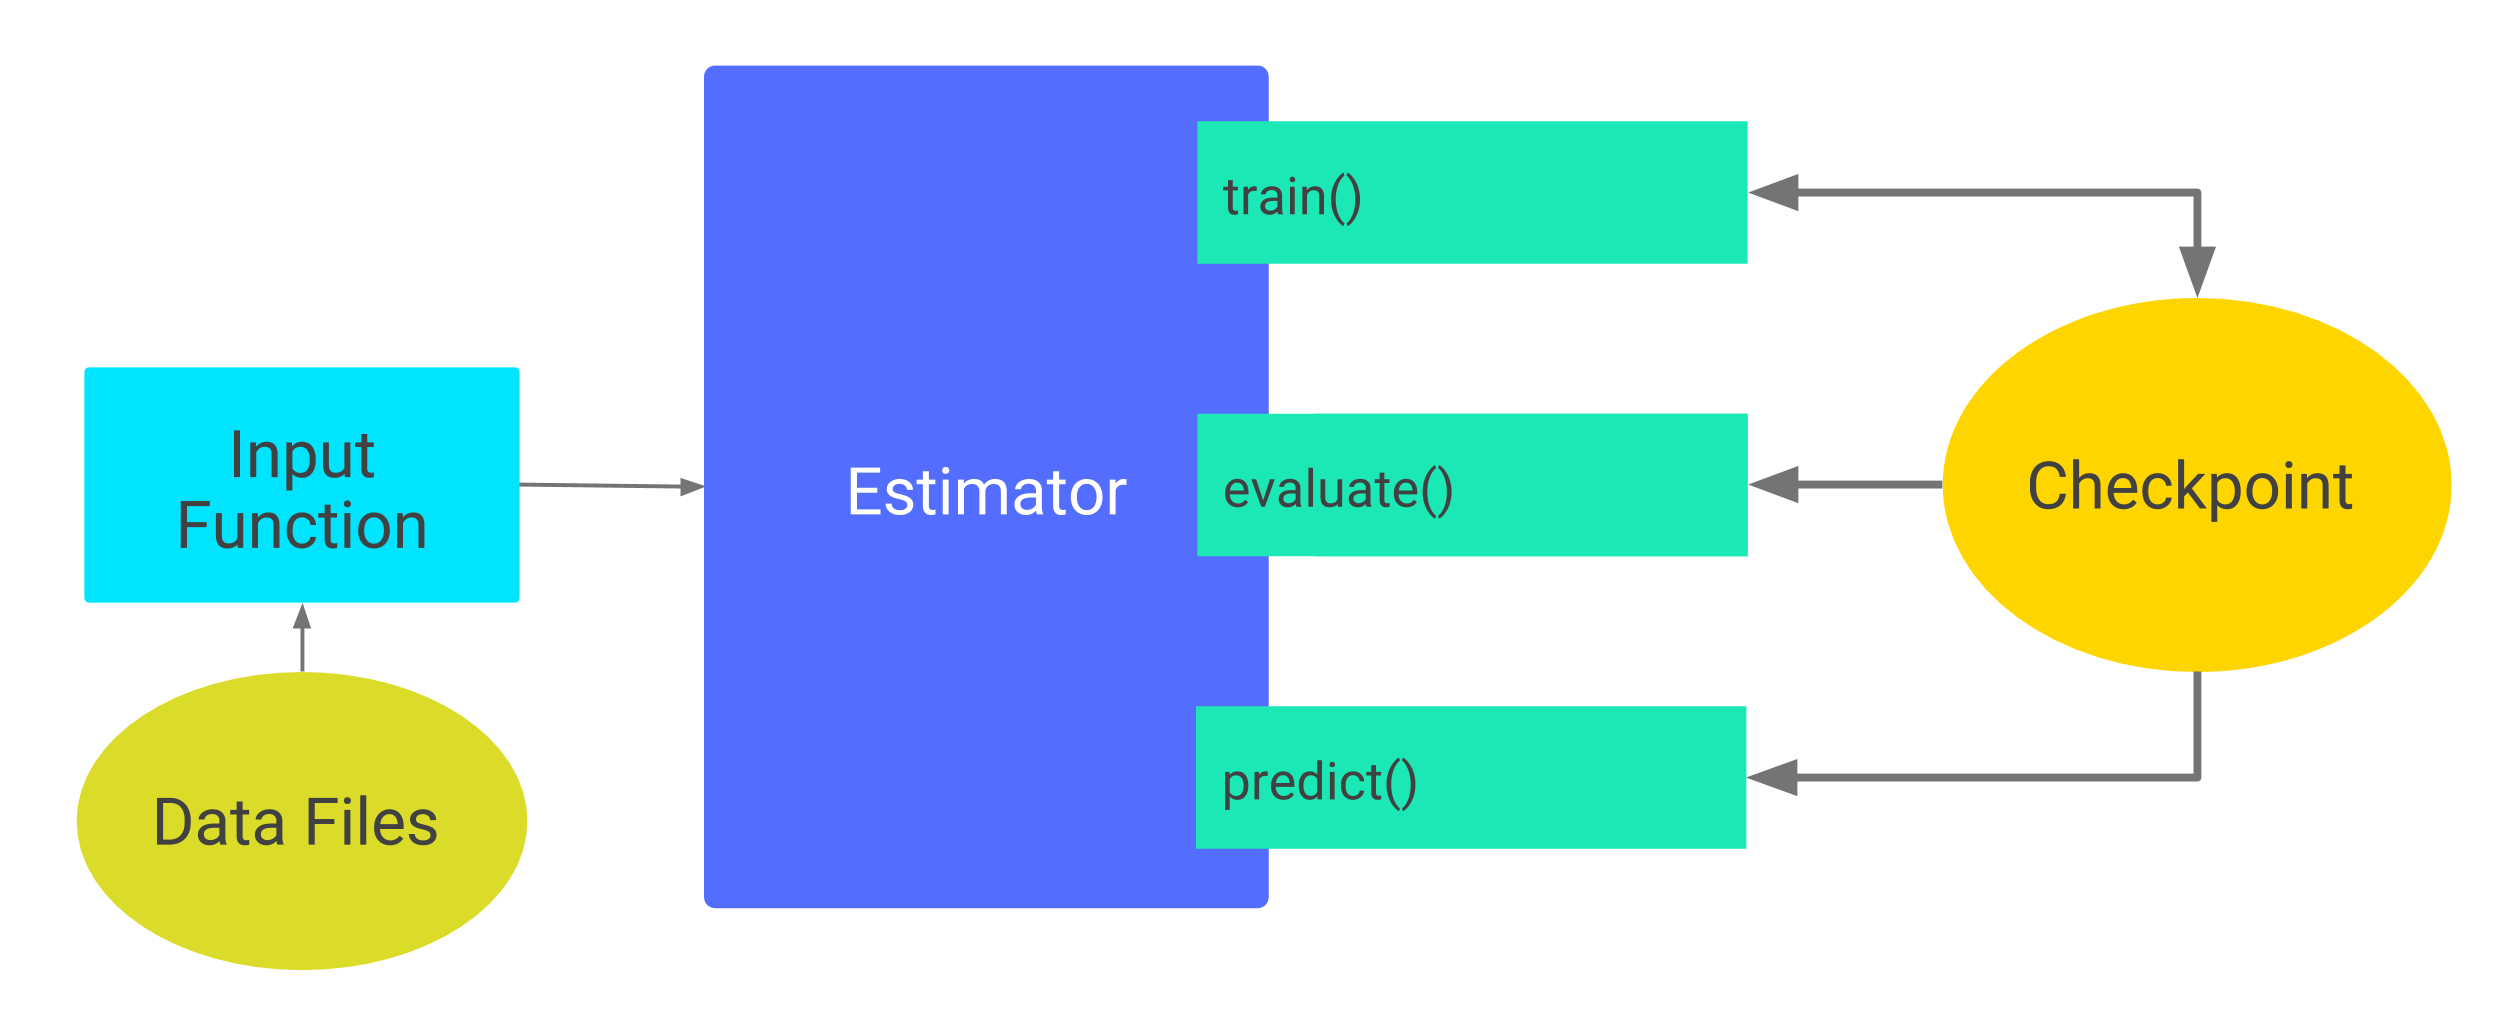
\includegraphics[height=6cm]{checkpoint.png}
  \captionof{figure}{Схема применения сериализациии и десериализации\cite{tf_doc:checkpoint}}\label{fig:func:checkpoint}
\end{center}

Так как поле \texttt{encoder} класса \texttt{cstlstm.ChildSumTreeLSTMClassifier} хранит ссылку на объект типа \texttt{cstlstm.ChildSumTreeLSTMCell}, но, при этом, объект типа \texttt{cstlstm.ChildSumTreeLSTMCell} может существовать независимо, то от класса \texttt{cstlstm.ChildSumTreeLSTMClassifier} направлена связь типа композиция в сторону класса \texttt{cstlstm.ChildSumTreeLSTMCell}. Данная композиция отображена на диаграмме классов, изображенной на чертеже ГУИР.400201.009.РР.1.

Класс \texttt{train.Treebank} контролируюет прогресс обработки некоторого набора данных. При создании объекта типа \texttt{train.Treebank} будет выгружен набор данных из базы данных или из файла. Затем, во время итерации по набору данных можно будет изображать прогресс выполнения с помощью вызова метода \texttt{print\_progress\_bar}. Данный метод будет рассчитывать текущий прогресс основываясь на публичном поле класса \texttt{train.Treebank} \texttt{size}, который хранит размер всего набора данных. Это необходимо, так как инструменты контроля набора данных в Tensorflow не поддерживают такой возможности. Так как класс \texttt{train.Treebank} используется при обработке набора данных классом \texttt{train.Train}, то от класса \texttt{train.Treebank} направлена связь типа ассоциация в сторону класса \texttt{train.Train}. Данная ассоциация отображена на диаграмме классов, изображенной на чертеже ГУИР.400201.009.РР.1. Код конструктора класса \texttt{train.Treebank} представлен ниже:
\medskip
\begin{lstlisting}[style=Python]
  def __init__(self, data_dir, set_name, embed_indexes):
    json_path = os.path.join(data_dir, 'json', set_name + '.json')
    set_path = os.path.join(data_dir, set_name)
    with codecs.open(json_path, encoding='utf-8') as f:
      trees = json.load(f)
    trees = [replace_words_by_index(tree, embed_indexes) for tree in trees]
    if set_name == 'train':
      trees = [tree for tree in trees if tree[0] != 2]
    self.size = len(trees)
    jsons = ''.join([json.dumps(tree) + '\n' for tree in trees])
    with open(set_path, 'w') as f:
      f.write(jsons)
    super(Treebank, self).__init__(set_path)
\end{lstlisting}
\medskip

Параметр конструктра \texttt{train.Treebank} \texttt{data\_dir} типа \texttt{str} --- путь к набору данных. Параметр \texttt{set\_name} типа \texttt{str} --- это название набора данных, которое будет отображаться в строке состояния. Параметр \texttt{embed\_indexes} типа \texttt{dict} --- это словарь соответствия слов индексам их векторов в матрице модели GloVe.

Класс \texttt{train.Train} контролирует процесс обучения модели Child-Sum Tree LSTM\@. Имеет следующие публичные поля:
\begin{itemize}
\item \texttt{epochs}
\item \texttt{learning\_rate}
\item \texttt{embedding\_learning\_rate}
\item \texttt{model}
\item \texttt{model\_optimizer}
\item \texttt{embedding\_optimizer}
\item \texttt{checkpoint}
\end{itemize}

Публичное поле \texttt{epochs} типа \texttt{int} класса \texttt{train.Train} хранит количество эпох обучения архитектуры Child-Sum Tree LSTM\@. За одну эпоху обучения модель обрабатывает весь тренировочный набор данных. Слишком низкое количество эпох может привести к недостаточному обучению модели. Слишком высокое, наоборот, может привести к переобучению. Либо же, если при оптимизации точность модели не будет сходиться, то большее количество эпох свыше какого-то порога сходимости не даст прироста производительности модели Child-Sum Tree LSTM\@. На рисунке~\ref{fig:func:epoches} показан пример зависимости ошибки нейронной сети от пройденных эпох обучения.

\begin{center}
  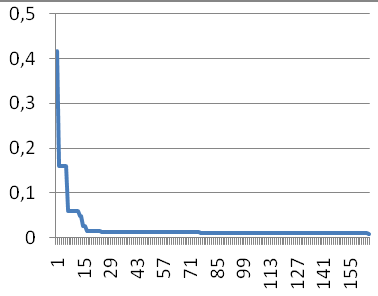
\includegraphics[height=6cm]{epoches.png}
  \captionof{figure}{Зависимость ошибки нейронной сети от количества пойденных эпох обучения\cite{Goodfellow-et-al-2016}.}\label{fig:func:epoches}
\end{center}

Публичное поле \texttt{learning\_rate} типа \texttt{float} класса \texttt{train.Train} хранит скорость обучения модели. Это коофициент в интервале [0, 1], который будет определять какая доля потери, вычислинной градиентным спуском, будет прибавлятся к тренируемым параметрам модели. На рисунке~\ref{fig:func:learning_rate} показаны зависимости ошибки от эпох обучения модели для разных скоростей обучения. Слишком низкая точность обучения может привести в тому, что модель может свестись только через черезмерно большое количество пройденных эпох обучения. Слишком большая скорость обучения может и вовсе привести к тому, что модель не сможет сойтись. Данный процесс изображен на рисунке~\ref{fig:func:learning_rate2}. Красной линией указана последовательность изменения весов модели нейронной сети.

\begin{center}
  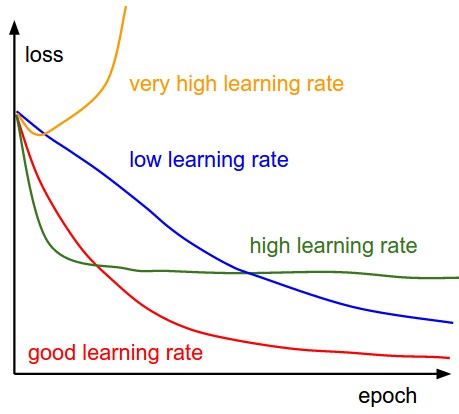
\includegraphics[height=6cm]{learning_rate.png}
  \captionof{figure}{Зависимость ошибки нейронной сети от количества пройденных этапов обучения, указанная для различных значений скорости обучения.\cite{stanford_course}.}\label{fig:func:learning_rate}
\end{center}

\begin{center}
  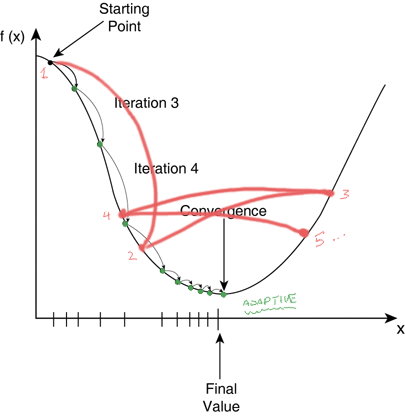
\includegraphics[height=6cm]{learning_rate2.png}
  \captionof{figure}{Сходимость функции потерь.\cite{stanford_course}.}\label{fig:func:learning_rate2}
\end{center}

Публичное поле \texttt{embedding\_learning\_rate\_factor} типа \texttt{float} класса \texttt{train.Train} хранит коэффициент замедления скорости обучения слоя проекции встраивания слов. Так как при обучении модели происходит дообучение векторов модели GloVe, то, чтобы сохранить стабильность системы, необходимо использовать замедление скорости обучения. Замедляется встраивание слов, так как оригинальная модель GloVe обучалась без учителся на огромных наборах данных очень долгое время. Поэтому быстрое обучение на наборе из десяти тысяч синтаксических деревьев зависимотсей нарушит стабильность модели GloVe.

Класс \texttt{train.Train} имеет публичное поле \texttt{model} типа \texttt{cstlstm.Child\-SumTreeLSTMClassifier}, которое хранит ссылку на объект модели Child-Sum Tree LSTM\@. Данный объект модели и будет обучаться средствами \texttt{train.Tra\-in}.

Публичное поле \texttt{model\_optimizer} типа \texttt{tensorflow.AdagradOptimiz\-er} класса \texttt{train.Train} является имплементацией алгоритма Адаграда для оптимизации. Он будет применяться для оптимизации обучаемых весов всей модели.

Однако скорость обучения модели Child-Sum Tree LSTM и скорость обучения модели GloVe отличаются, и алгоритм оптимизации должен в разной степени влиять на веса в модели Child-Sum Tree LSTM и модели GloVe. Публичное поле \texttt{enbedding\_optimizer} типа \texttt{tensorflow.AdagradOptimizer} класса \texttt{train.Train} является имплементацией алгоритма оптимизации Ада\-града. Оптимизатор \texttt{model\_optimizer} применяется для следующих параметров:
\begin{itemize}
\item ядро слоя вычисления сигнала забывания Сhild-Sum Tree LSTM\@;
\item смещение слоя вычисления сигнала забывания Child-Sum Tree LSTM\@;
\item ядро слоя вычисления врат ячейки Child-Sum Tree LSTM\@;
\item смещение слоя вычисления врат ячейки Child-Sum Tree LSTM\@;
\item ядро слоя трансформации входов ячейки Child-Sum Tree LSTM\@;
\item смещение слоя вычисления трансформации входов ячейки Child-Sum Tree LSTM\@;
\item ядро логистической регрессии модели Child-Sum Tree LSTM\@;
\item смещение логистической регрессии модели Child-Sum Tree LSTM\@.
\end{itemize}
Оптимизатор \texttt{embed\_optimizer} применяется для следующих параметров:
\begin{itemize}
\item ядро плотного слоя проекции векторов GloVe модели Child-Sum Tree LSTM\@;
\item смещение плотного слоя проекции векторов GloVe модели Child-Sum Tree LSTM\@.
\end{itemize}

Публичное поле \texttt{checkpoint} типа \texttt{tensorflow.Checkpoint} класса \texttt{tra\-in.Train} является сериализатором модели Child-Sum Tree LSTM\@.

Класс \texttt{train.Train} хранит ссылку на объект класса \texttt{cstlstm.ChildSum\-TreeLSTMClassifier} и является независимым, поэтому от класса \texttt{train.Tra\-in} направлена связь типа агрегации в сторону класса \texttt{cstlstm.ChildSumTree\-LSTMClassifier}. Данная агрегация отображена на диаграмме классов, изображенной на чертеже ГУИР.400201.009.РР.1.

Ниже показан конструктор класса \texttt{train.Train}:
\medskip
\begin{lstlisting}[style=Python]
  def __init__(self, epochs, learning_rate, embedding_learning_rate_factor, checkpoint_dir, embed_dir):
    self.epochs = epochs
    self.learning_rate = learning_rate
    self.embedding_learning_rate_factor = embedding_learning_rate_factor

    embed, embed_indexes = self.load_embeddings(embed_dir)
    model = ChildSumTreeLSTMClassifier(embed)
    model_optimizer = tf.train.AdagradOptimizer(learning_rate)
    embedding_optimizer = tf.train.AdagradOptimizer(learning_rate * embedding_learning_rate_factor)
    checkpoint = model.checkpoint()
\end{lstlisting}
\medskip

Класс \texttt{train.Train} обладает следующими публичными методами:
\begin{itemize}
\item \texttt{replace\_words\_by\_index};
\item \texttt{train\_epoch};
\item \texttt{dev\_eval};
\item \texttt{evaluate\_dataset};
\item \texttt{load\_embedding}.
\end{itemize}

Публичный метод \texttt{replace\_words\_by\_index(tree, word2index)} класса \texttt{train.Train} заменяет слова в синтаксическом дереве зависимостей на индексы соответствующих им векторов в матрице отфильтрованных векторов GloVe. Данная операция необходима, чтобы во время обработки дерева воспользоваться средствами Tensorflow для загрузки плотных векторов.  Метдо получает параметр \texttt{tree} типа \texttt{list}, в котором хранится синтаксическое дерево зависимостей. Так же метод получает параметр \texttt{word2index} типа \texttt{dict}, где хранится соответствие слов из модели GloVe индексам их плотных векторов. Метод возвращает \texttt{list} в котором хранится исходное дерево, где слова заменены индексам векторов GloVe.

Публичный метод \texttt{train\_epoch} класса \texttt{train.Train} имеет следующие входные параметры:
\begin{itemize}
\item \texttt{model};
\item \texttt{train\_trees};
\item \texttt{model\_optimizer};
\item \texttt{embedding\_optimizer};
\item \texttt{batch\_size}.
\end{itemize}

Итак, метод \texttt{train\_epoch(model, train\_trees, model\_optimizer, embedding\_optimizer, batch\_size=25)} реализует эпоху обучения модели Child-Sum Tree LSTM\@. Параметр \texttt{model} типа \texttt{cstlstm.ChildSumTreeLSTMCla\-ssifier} хранит обучаемую модель Child-Sum Tree LSTM\@. Параметр \texttt{train\-\_trees} содержит тренировочный набор синтаксических деревьев зависимостей, которые хранятся в формате JSON\@, с заменнеными словами на индексы соответствующих им векторам GloVe. Параметр \texttt{model\_optimizer} типа \texttt{tensorflow.AdagradOptimizer} содержит имплементацию оптимизационного метода Адаграда для модели анализа тональностей в тексте Child-Sum Tree LSTM\@. Параметр \texttt{embedding\_optimizer} типа \texttt{tensorflow.AdagradOptimizer} содержит имплементацию оптимизационного метода Адаграда для модели встраивания слов GloVe. Параметр \texttt{batch\_size} содержит размер группы деревьев из набора данных. Тренировочный набор разбивается на группы в ходе тренировочной эпохи. После обработки каждой группы будет высчитываться градиент и оптимизироваться веса модели Child-Sum Tree LSTM\@. Размер группы --- это один из гиперпараметров модели. Большой размер группы ускорит эпоху обучения, так как количество групп, на которые поделен тренировочный набор равняется количеству оптимизаций модели, производимых за одну эпоху. Однако, чем меньше оптимизаций проводится, тем медленнее обучается модель, и при слишком большом размере группы оптимизатор будет делать слишком общие выводы для большого числа входных данных, а процесс обучения будет требовать большего количества эпох. При слишком маленьком размере группы время вычислений одной эпохи сильно возрастает, помимо этого оптимизатор будет длеать выводы на основе малого количества входных данных и модель будет подстраиваться под слишком индивидуальные особенности треднировочных данных, что может привести к переобучению. Влияение размера группы на процесс обучения отображено на рисунке~\ref{fig:func:batch_size}. Помимо примера большого и маленького размера группы, так же указан пример для случайного размера группы --- Stochastic Batch Size.

\begin{center}
  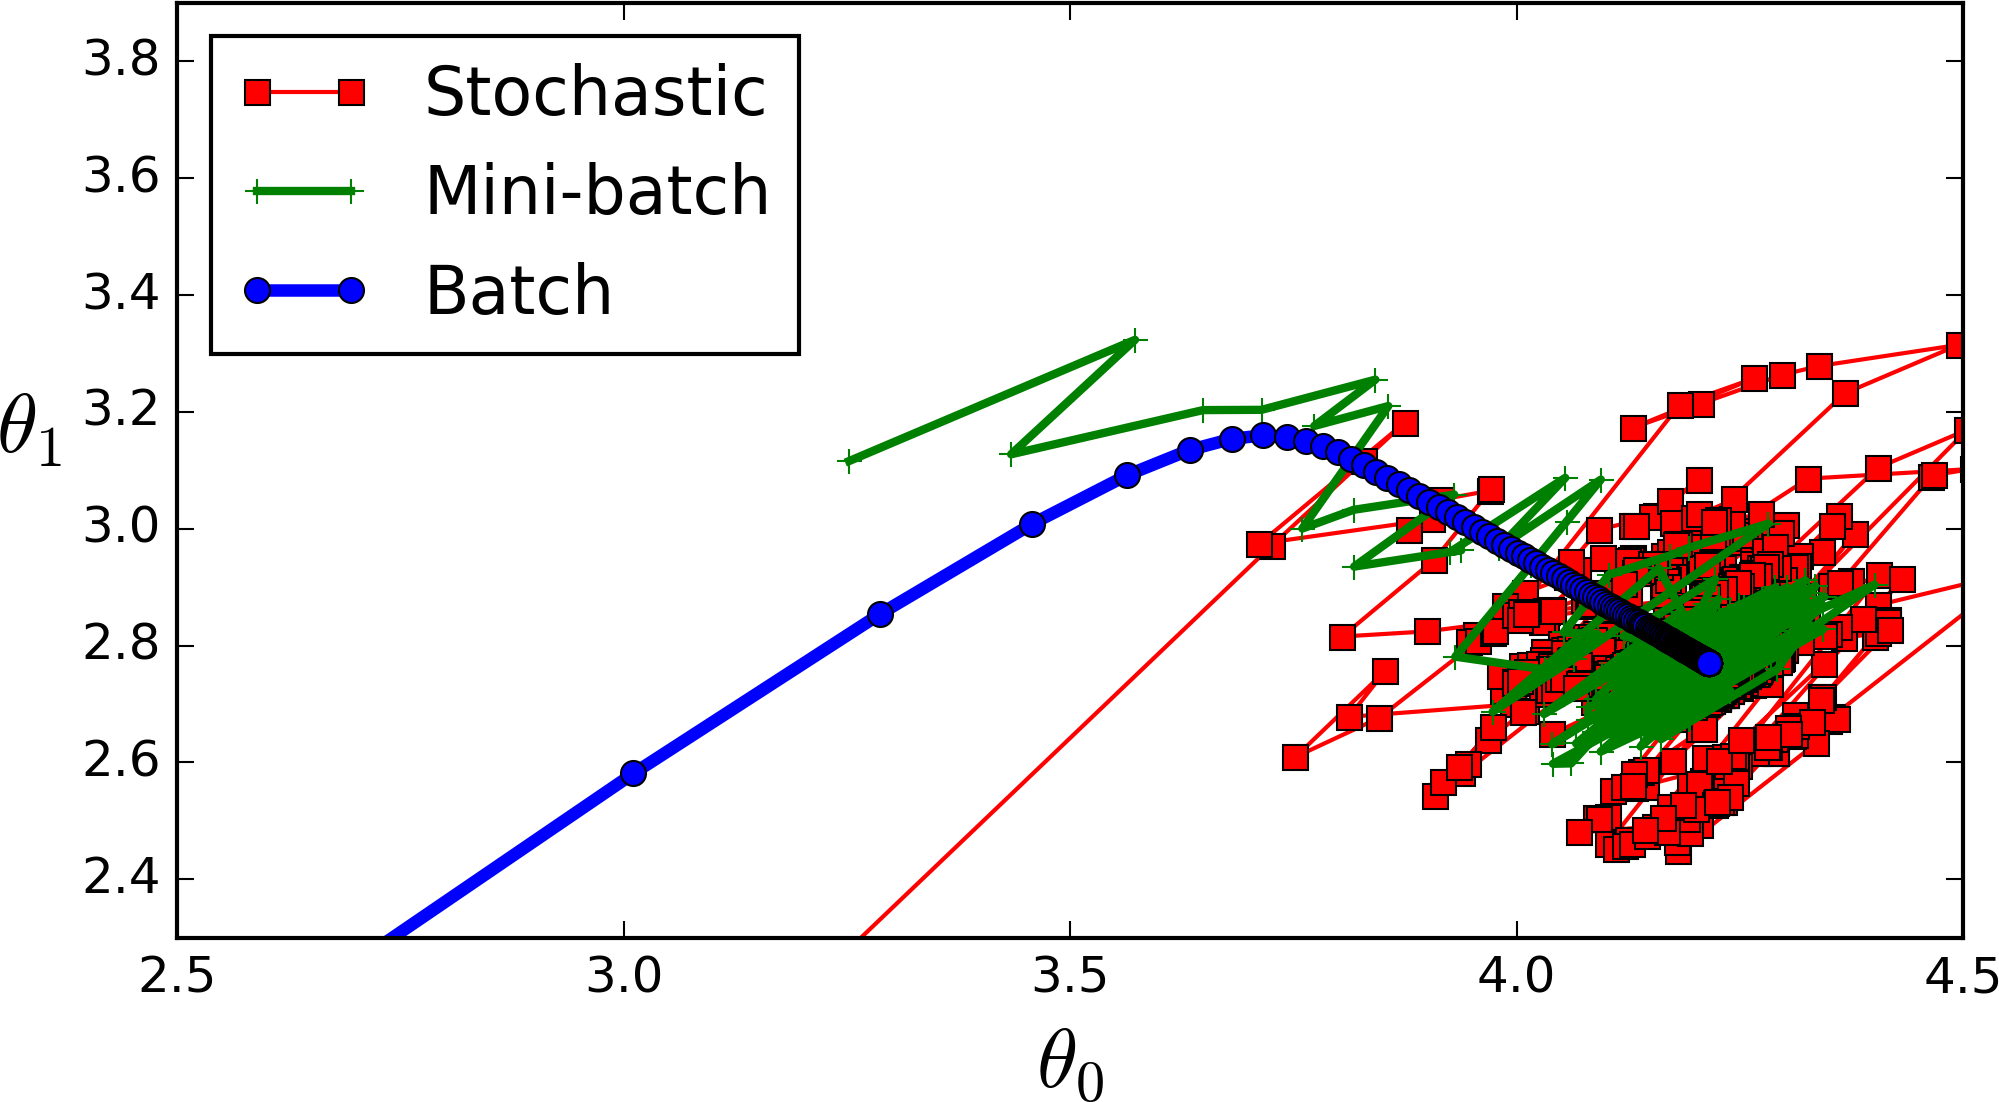
\includegraphics[height=6cm]{batch_size.png}
  \captionof{figure}{Влияение размера группы на процесс обучения.\cite{stanford_course}.}\label{fig:func:batch_size}
\end{center}

Публичный метод \texttt{dev\_eval} класса \texttt{train.Train} имеет следующие входные параметры:
\begin{itemize}
\item \texttt{model};
\item \texttt{epoch};
\item \texttt{dev\_trees};
\item \texttt{train\_loss}.
\end{itemize}

Метод \texttt{dev\_eval(model, epoch, dev\_trees, train\_loss)} реализует обработку набора данных dev, который предназначен для настройки гиперпараметров модели. Так как гиперпараметры настраиваются специалистом на основе результатов работы системы, то метод \texttt{dev\_eval} просто выводит всевозможные метрики и информацию о ошибках модели. Пареметр \texttt{model} типа \texttt{cstlstm.ChildSumTreeLSTMClassifier} хранит обучаемую модель Child-Sum Tree LSTM\@ Параметр \texttt{epoch} типа \texttt{int} хранит номер этохи обучения. В параметре \texttt{dev\_trees} типа \texttt{list} хранятся синтаксические деревья зависимостей, сохраненные в json фомате. Параметр \texttt{train\_loss} типа \texttt{float} хранит значение функции потерь модели за текущую эпоху обучения.

Публичный метод \texttt{evaluate\_dataset(model, trees, batch\_size=25)} класса \texttt{train.Train} реализует обработку набора данных синтаксических деревьев зависимостей. Пареметр \texttt{model} типа \texttt{cstlstm.ChildSumTreeLSTMCla\-ssifier} хранит обучаемую модель Child-Sum Tree LSTM\@. В параметре \texttt{trees} типа \texttt{list} хранятся синтаксические деревья зависимостей, сохраненные в json фомате. Параметр \texttt{batch\_size} содержит размер группы деревьев из набора данных. Набор синтаксических деревьев зависимостей разбивается на группы в ходе обработке набора, и модель выполняется для всех деревьев одной группы одновременно. Метод возвращает средние значения точности для:
\begin{itemize}
\item классификации на 5 классов для корневых узлов деревьев;
\item классификации на 5 классов для всех узлов деревьев;
\item бинарной классификации на для корневых узлов деревьев;
\item бинарной классификации на для всех узлов деревьев.
\end{itemize}

Класс \texttt{train.Train} владеет публичным методом \texttt{load\_embeddings(em
  -bedding\_path)}, который реализует загрузку модели встаивания слов GloVe. Единственный входной параметр \texttt{embedding\_path} типа \texttt{str} хранит путь к модели GloVe. Метод возвращает матрицу типа \texttt{tensorflow.Tensor}, где хранятся плотные векторы слов, и словарь типа \texttt{dict}, который хранит соответсвие слов индексам их плотных векторов в матрице модели GloVe.

Класс \texttt{inference.Inference} управляет процессом предсказаний с помощью обученной модели Child-Sum Tree LSTM\@. Имеет следующие публичные поля:
\begin{itemize}
\item \texttt{model};
\item \texttt{tree};
\item \texttt{result};
\item \texttt{pretty\_tree}.
\end{itemize}

Код конструктора класса \texttt{inference.Inference} показан ниже:

\medskip
\begin{lstlisting}[style=Python]
  def __init__(self, path_to_jar, path_to_models_jar, sentence, embed_path, checkpoint_path):
    dependency_parser = StanfordDependencyParser(path_to_jar=path_to_jar, path_to_models_jar=path_to_models_jar)
    tokens = nltk.word_tokenize(sentence)
    tree = dependency_parser.parse_one(tokens)
    tree = tree.tree()

    embed, embed_indexes = load_embeddings('./data/filtered_glove.txt')
    self.model = ChildSumTreeLSTMClassifier(embed)
    checkpoint = model.checkpoint()
    checkpoint.restore(tf.train.latest_checkpoint(checkpoint_directory))
    self.tree = json.dumps(tree_to_list(tree, embed_indexes))
    self.result = []
    self.pretty_tree = None
\end{lstlisting}
\medskip

Входные параметра конструктора \texttt{inference.Inference}:
\begin{itemize}
\item \texttt{path\_to\_jar};
\item \texttt{path\_to\_directory};
\item \texttt{sentence};
\item \texttt{embed\_path};
\item \texttt{checkpoint\_path}.
\end{itemize}

Параметр \texttt{path\_to\_jar} типа \texttt{str} хранит путь к программе синтаксического анализатора CoreNLP\@. Парметр \texttt{path\_to\_models\_jar} типа \texttt{str} задает путь к модели shift reduce синтаксического анализатора зависимостей. Параметром \texttt{sentence} типа \texttt{str} задается предложение, которое необходимо обработать. Параметр \texttt{embed\_path} типа \texttt{str} хранит путь к модели встраивания слов GloVe. Параметр \texttt{checkpoint\_path} типа \texttt{str} хранит путь к модели Child-Sum Tree LSTM\@.

Публичное поле \texttt{model} класса \texttt{inference.Inference} типа \texttt{cstlstm.Ch\-ildSumTreeLSTMClassifier} хранит модель Child-Sum Tree LSTM\@. Так как класс \texttt{inference.Inference} хранит ссылку на объект класса \texttt{cstlstm.Child\-SumTreeLSTMClassifier}, однако, при удалении объекта модели, объект предсказателя дожен сохраняться, то от класса \texttt{inference.Inference} направлена связь типа агрегация в сторону класса \texttt{cstlstm.ChildSumTreeLSTMClassifi\-er}. Данная агрегация отображена на диаграмме классов на чертеже ГУИР. 400201.009.РР.1.

Публичное поле \texttt{tree} класса \texttt{inference.Inference} типа \texttt{str} хранит синтаксическое дерево зависимостей анализируемого предложения в формате JSON\@.

Публичное поле \texttt{result} класса \texttt{inference.Inference} типа \texttt{int[]} хранит результаты аналзиа тональностей дерева для каждого узла синтаксического дерева зависимостей. Результаты предсказаний храняться в развертке, в последовательности соответствующей порядку обхода дерева методо поиска в глубину.

Публичное поле \texttt{pretty\_tree} класса \texttt{inference.Inference} типа \texttt{visu\-alization.LabeledTree} хранит ссылку на объект дерева, подлежащего визуализации с помощью \texttt{visualization.Visualizator}. Так как предсказатель может существовать независимо от дерева визуализации, то от класса \texttt{infer\-ence.Inference} направлена связь типа агрегация в сторону класса \texttt{visuali\-zation.LabeledTree}. Данная агрегация отображена на диаграмме классов на чертеже ГУИР.400201.009.РР.1.

Класс \texttt{inference.Inference} обладает следующими публичными методами:
\begin{itemize}
\item \texttt{tree\_to\_list(tree, embed\_indexes)};
\item \texttt{load\_embeddings(embedding\_path)};
\item \texttt{convert\_result(tree, results)}.
\end{itemize}

Публичный метод \texttt{tree\_to\_list(tree, embed\_indexes)} класса \texttt{infe\-rence.Inference} преобразует дерево из формата, возращаемого синтаксическим анализатором CoreNLP в входной формат модели Child-Sum Tree LSTM\@. Параметр \texttt{tree} типа \texttt{nltk.Tree} хранит дерево в фомате CoreNLP\@. Параметр \texttt{embed\_indexes} типа \texttt{dict} сранит словарь соответствий слов их плотным векторам в модели GloVe.

Публичный метод \texttt{load\_embeddings(embedding\_path)} класса \texttt{infere\-nce.Inference} реализует загрузку модели встаивания слов GloVe. Единств\-енный входной параметр \texttt{embedding\_path} типа \texttt{str} хранит путь к модели GloVe. Класс \texttt{train.Train} преобразует модель GloVe к тензору Tensorflow, но в реализации этого метода класса \texttt{Inference} нет необходимости в поиске плотных векторов слов во время выполнения модели Child-Sum Tree LSTM, так как предсказатель работает только с одинм деревом.

Публичный метод \texttt{convert\_result(tree, results)} класса \texttt{Inference} преобразует синтаксическое дерево зависимостей в формат, пригодный для визуализации. Параметр \texttt{tree} типа \texttt{list} хранит дерево в формате модели Child-Sum Tree LSTM\@. Параметр \texttt{results} хранит результаты работы системы анализа тональностей в последовательности обхода синтаксического дерева методом поиска в глубину. Метод \texttt{convert\_result(tree, results)} возвращает дерево в пригодном для визуализации формате типа \texttt{visualization.La\-beledTree}.

\subsection{Модуль визуализации TensorBoard}
Модуль визуализации TensorBoard представляет собой отдельно приложение, которое визуализирует внутренние процессы, протекающие в модели машинного обучения. Поэтому этот модуль визуализации не имеет представления на диаграмме классов. В код проекта он ключен только в виде специальных меток, позволяющий TensorBoard собирать информацию о модели.

\subsection{Модуль визуализации CoreNLP}
Модуль визуализации CoreNLP выводит синтаксическое дерево зависимостей обработанного предложения и демонстрирует последовательность, в которой модель Child-Sum Tree LSTM делала выводы. Модуль представлен двумя классами:
\begin{itemize}
\item \texttt{visualization.LabeledTree};
\item \texttt{visualization.Visualizator}.
\end{itemize}

Класс \texttt{visualization.LabeledTree} представляет синтаксическое дерево зависимостей с предсказанными уровнями тональностей для кахдой фразы в предложении. Класс имеет следующие публичные поля:
\begin{itemize}
\item \texttt{label};
\item \texttt{children};
\item \texttt{text};
\item \texttt{parent};
\item \texttt{depth}.
\end{itemize}

Публичное поле \texttt{label} типа \texttt{int} класса \texttt{visualization.LabeledTree} содержит значение тональности для данного дерева. Поле \texttt{children} типа \texttt{vi\-sualization.LabeledTree[]} хранит ссылки на объекты данного класса, которые являются детьми текущего объекта. Поле \texttt{parent} типа \texttt{visualizati\-on.LabeledTree} содержит ссылку ссылку на объект узла-родителя текущего дерева. Таким образом содается древовидная структура, каждый узел которой является объектом класса \texttt{visualization.LabeledTree}. Поле \texttt{text} типа \texttt{str} хранит слово или фразу, соответствующее текущему узлу. Поле \texttt{depth} типа \texttt{int} хранит глубину текущего дерева. Это необходимо для операций нормализации дерева.

Код конструктора класса \texttt{visualization.LabeledTree} предствлен ниже:
\medskip
\begin{lstlisting}[style=Python]
    def __init__(self, depth=0, text=None, label=None, children=None, parent=None):
        self.label    = label
        self.children = children if children != None else []
        self.general_children = []
        self.text = text
        self.parent   = parent
        self.depth    = depth
\end{lstlisting}
\medskip

Публичный метод \texttt{add\_child(child)} класса \texttt{visualization.Labeled\-Tree} добваляет узел в список детей текущего узла. Параметр \texttt{child} типа \texttt{vi\-sualization.LabeledTree} хранит объект дерева, которое будет добавлено в список детей.

Публичный метод \texttt{to\_dict()} класса \texttt{visualization.LabeledTree} преобразует текущее дерево в словарь, который хранит всю необходимую информацию и позволяет воссоздать дерево из солваря без потери информации. Метод возвращает объект типа \texttt{dict}.

Публичный метод \texttt{to\_json()} класса \texttt{visualization.LabeledTree} сериализует текущее дерево в формат JSON. Метод возвращает объект типа \texttt{str}.

% \section{РАЗРАБОТКА ПРОГРАММНЫХ МОДУЛЕЙ}
\label{sec:development}
При разработке системы одними из наиважнейших требований к исходному коду являются его расширяемость и поддерживаемость. Реализация программных модулей с учетом этих требований приводит к простоте расширения функционала в критических местах, обеспечению разделенности и независимости компонентов системы, что улучшает их тестируемость и в целом позволяет добиться реализации более стабильной и простой в понимании кодовой базы.

\subsection{Слой Child-Sum Tree LSTM}
Итак, задача модели Child-Sum Tree LSTM в том, чтобы применить слой Tree LSTM к дереву, обходя его последовательно от литьев к корню. На каждом этапе слой принимает на вход плотный вектор входного слова и набор векторов состояний дочерних узлов синтаксического дерева. Плотный вектор слова это постоянный параметр, в то время как вектора дочерних узлов могут и отсутствовать. Таким образом необходимо выполнять вычисления только для тех узлов, для которых уже известны значения состояний их дочерних узлов.

Затем, после того как рассчитан плотный вектор, соответствующий всему предложению, необходимо найти разницу между полученным значением, и эталонным значением. Эта разница выражается функцией потерь. Значение потерь необходимо минимизировать. Поэтому производится оптимизация функции потерь, экстремум функции потерь в зависимости от обучаемх параметров модели. Затем параметры модели изменяются таким образом, чтобы уменьшить среднее значение функции потерь. Данный процесс отображен на рисунке~\ref{fig:dev:slide}.

\begin{center}
  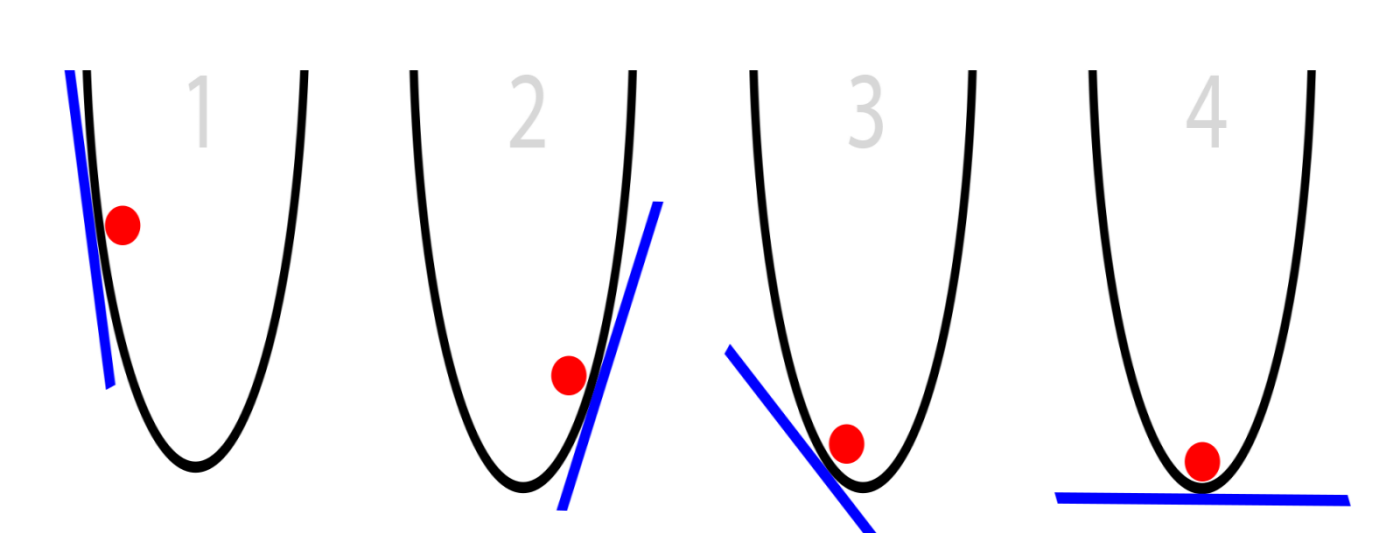
\includegraphics[height=6cm]{sliding_gradient.png}
  \captionof{figure}{Демонстрация оптимизации функции\cite{Goodfellow-et-al-2016}}\label{fig:dev:slide}
\end{center}

Очевидно, что это очень сложный вычислительный процесс, поэтому часто в машинном обучении приходят к оптимизации вычислений на графических процессорах. Для этого в проекте был использован фреймворк Tensor\-flow, позволяющий оптимизировать вычисления на графических процессорах.

Проблема в том, что графический процессор работает с собственным устройством памяти. На рисунке~\ref{fig:dev:cpu_gpu_mem} показана схема перемещения данных между процессорами. Если передавать графическому процессору только математические операции, а все управление производить с помощью центрального процессора, то ускоренные математические вычисления могут и не дать общего прироста производительности, за счет потерь при перемещении данных с одного устройства памяти на другое. С другой стороны, если передать целиком управление графическому устройству, то это очень сильно усложнит процесс разработки. Так как разработчику доступена только оперативная память центрального процессора, то будет возможность только увидеть результат вычислений на графическом процессоре. Промежуточные результаты вычислений и отладка недоступны.

\begin{center}
  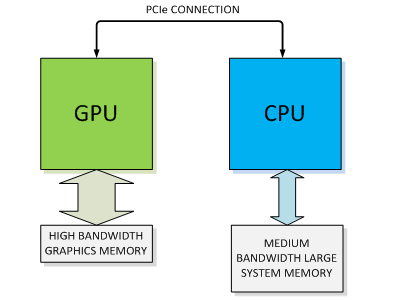
\includegraphics[height=8cm]{cpu_gpu_mem.png}
  \captionof{figure}{Схема перемещения данных в вычислениях на графических процессорах\cite{Goodfellow-et-al-2016}}\label{fig:dev:cpu_gpu_mem}
\end{center}

Tensorflow представляет разработчику высокоуровневое API keras, а управление в большей степени производит самостоятельно. Итак, класс \texttt{cst\-lstm.ChildSumTreeLSTM} является наследником класса \texttt{keras.Layers.Model}. Таким образом класс ячейки Child-Sum Tree LSTM становится одним из блоков Tensorflow и контролируется фреймворком. Алгоритм вычислений, которые производит модель, задан в перегруженной функции \texttt{call}, код которой указан ниже:
\medskip
\begin{lstlisting}[style=Python]
  def call(self, inputs, *args, **kwargs):
    input_word, child_c, child_h = inputs
    child_h_sum = tf.reduce_sum(child_h, 0)
    concat = tf.concat([input_word, child_h_sum], 1)
    i, o, u = tf.split(self.iou_signals(concat), 3, axis=1)
    i, o, u = tf.sigmoid(i), tf.sigmoid(o), tf.tanh(u)
    f = self.forget_signals(child_h) + self.input_transform(input_word) + self.forget_bias
    f = tf.sigmoid(f)
    c = (i * u) + tf.reduce_sum(f * child_c, 0)
    h = o * tf.tanh(c)
    return c, h
\end{lstlisting}
\medskip

Для удобства вычилсений произведены приобразование рассчетов состояний нейронов в узле Child Sum Tree LSTM следующим образом:
\begin{gather}
  \label{eq:func:lstm:i}
  i_{jk} = \sigma(W^{(i)}\cdot{x_j} + U^{(i)}\cdot{\tilde{h_j}} + b^{(i)}) = \sigma({V^{(i)}\cdot{
      \begin{bmatrix}
        x_j\\
        h_j
      \end{bmatrix}} + b^{(i)}}),\\
  \label{eq:func:lstm:forget}
  f_{jk} = \sigma(W^{(f)}\cdot{x_j} + U^{(f)}\cdot{h_k} + b^{(f)}) = \sigma({V^{(f)}\cdot{
      \begin{bmatrix}
        x_j\\
        h_j
      \end{bmatrix}} + b^{(f)}}),\\
  \label{eq:func:lstm:o}
  o_{jk} = \sigma(W^{(o)}\cdot{x_j} + U^{(o)}\cdot{h_j} + b^{(o)}) = \sigma({V^{(o)}\cdot{
      \begin{bmatrix}
        x_j\\
        h_j
      \end{bmatrix}} + b^{(o)}}),\\
  \label{eq:func:lstm:u}
  u_{jk} = \sigma(W^{(u)}\cdot{x_j} + U^{(u)}\cdot{h_j} + b^{(u)}) = \sigma({V^{(u)}\cdot{
      \begin{bmatrix}
        x_j\\
        h_j
      \end{bmatrix}} + b^{(u)}}),\\
  \label{eq:func:lstm:transform}
  c_j = i_j\odot{u_j} + \sum_{k\in{C(j)}}f_{jk}\odot{c_k},
\end{gather}
\begin{explanationx}
\item [где]       $\begin{bmatrix}x_j\\h_j\end{bmatrix}$ --- конкатенация векторов $x_j$ и $h_j$;
\item $V$ --- это конкатенация матриц весов $W$ и $H$.
\end{explanationx}

Параметр \texttt{inputs} представляет собой \texttt{Tuple} в котором хранятся: вектор входного слова, набор векторов состояний ячеек дочерних узлов и набор векторов состояний внутреннего слоя дочерних узлов. Первыя операция и заключается в том, чтобы извлечь из \texttt{inputs} эти три параметра. Такой формат необходим из-за того, что \texttt{cell} --- это перегруженная функция класса предка \texttt{keras.Layers.Model}. Следующий шаг заключается в том, чтобы суммировать состояния внутренних слоев дочерних узлов. Затем, плотный вектор входного слова и данная сумма конкатинируются в один вектор \texttt{concan}. Это позволит вычислить результат одной операцией Tensorflow, куда передастся этот конкатинированный вектор, вместо двух, куда бы передавлася каждый вектор последовательно. Затем, данный вектор \texttt{concat} передается полносвязному слою \texttt{iou\_signals} и результать вычислений разбивается на три равных вертора с помощью функции \texttt{tensorflow.split}. Эти три вектора соответствуют трем сигналам LSTM\@:
\begin{itemize}
\item input сохраняется в переменную \texttt{i};
\item output сохраняется в переменную \texttt{o};
\item update сохраняется в переменную \texttt{u}.
\end{itemize}

Затем к каждому сигналу применяется функция активации. Для input и output функция активации --- это сигмодиа, реализованная \texttt{tensorflow.sig\-moid}, для update --- тангенс, реализованный \texttt{tensorflow.tanh}. Далее строится промежуточная матрица сигнала забывания forget и сохраняется в переменную \texttt{f}. Матрица состояний скрытых слоев дочерних узлов передается в полносвязный слой \texttt{forget\_signals}. Плотный вектор входного слова передается полносвязному слою \texttt{input\_transform}. Каждая строка результирующей матрицы \texttt{forget\_signals} суммируется с выходным вектором \texttt{input\_trans\-form} и к каждому элементу прибавляется \texttt{forget\_bias} --- смещение сигнала забывания.

Затем к промежточной матрице сигнала забывания применяется функция активации сигмоида. Потом получается произведение Адамара данной матрицы с матрицей состояний ячеек дочерних узлов --- \texttt{f * child\_c}. Матрица в результате произведения передается в \texttt{tensorflow.reduce\_sum}, которая сложит все строки матрицы. Затем, произведение Адамара применяется к сигналам input и update. И полученные два вектора складываются и в результате получается состояние ячейки Child-Sum Tree LSTM\@.

Вектор состояния ячейки передается в функцию активации, в данном случае --- тангенс, и результат умножается произведением Адамара на вектор сигнала output. Таким образом будет получен вектор состояния скрытого слоя текущего узла. Состояния скрытого слоя и состояния ячейки вызвращаются из функции.

\subsection{Модель Child-Sum Tree LSTM}
Класс \texttt{cstlstm.ChildSumTreeLSTMClassifier} также является наследником \texttt{keras.Layers.Model}. Поэтому обработка начинается с метода \texttt{call}:
\medskip
\begin{lstlisting}[style=Python]
  def call(self, inputs, training=None, *args, **kwargs):
    out = tf.map_fn(lambda tree: self.eval_tree(json.loads(tree.numpy())), inputs, dtype='int32')
\end{lstlisting}
\medskip

Параметр \texttt{inputs} содержит входные синтаксческие деревья зависимостей, в которых слова заменены индексами их векторов в матрице модели GloVe. Данные синтаксические деревья сохранены в формате JSON, чтобы их можно было лекго упаковать в структуру \texttt{tensorflow.Tensor} с виде строк. Функция \texttt{tensorflow.map\_fn} будет применять переданную ей функцию к каждому элементу переданного в неё тензора. Входной тензор и будет тензор JSON синтаксических деревьев из \texttt{inputs}. Входная функция передана в виде \texttt{lambda} выражения, которое применится для каждого дерева в тензоре. То есть сперва применяется распаковка JSON \texttt{json.loads}, а потом применяется функция обработки деревьев \texttt{eval\_tree}.

Метод \texttt{reset\_metrics} сбрасывает статистику обработанных деревьев для модели:
\medskip
\begin{lstlisting}[style=Python]
  def reset_metrics(self):
    self.loss = 0
    self.result = []
    self.fine = tfe.metrics.Accuracy()
    self.binary = tfe.metrics.Accuracy()
    self.root_fine = tfe.metrics.Accuracy()
    self.root_binary = tfe.metrics.Accuracy()
\end{lstlisting}
\medskip

Функция \texttt{eval\_tree} обрабатывает синтаксическое дерево зависимостей и делает предсказание тональности для отдельных фраз в предложении и для всего предложения целиком. Описание функции представлено ниже:
\medskip
\begin{lstlisting}[style=Python]
  def eval_tree(self, tree, is_root=True):
    sentiment = tree[0]
    word = tree[1][0]
    childs = tree[1][1]
    if word == -1:
      word_embed = tf.random_uniform((self.embed.shape[1],), -0.05, 0.05)
    else:
      word_embed = tf.nn.embedding_lookup(self.embed, word)
    word_embed = tf.reshape(word_embed, (1, word_embed.shape[0]))
    word_embed = self.projection(word_embed)
    word_embed = self.dropout(word_embed)
    child_h = []
    child_c = []
    for child in childs:
      child_state = self.eval_tree(child, is_root=False)
      child_c.append(child_state[0])
      child_h.append(child_state[1])
    if childs:
      child_c = tf.convert_to_tensor(child_c)
      child_h = tf.convert_to_tensor(child_h)
    else:
      child_c = tf.zeros((1, 1, self.encoder.unit_number))
      child_h = tf.zeros((1, 1, self.encoder.unit_number))
    child_state = self.encoder([word_embed, child_c, child_h])
    logits = self.output_layer(child_state[1])
    self._add_metrics(sentiment, logits)
    if is_root:
      prediction = tf.cast(tf.argmax(logits[0]), tf.int32)
      self.result.append(prediction)
      self.root_fine(sentiment, prediction)
      if sentiment != 2:
        self.root_binary(int(sentiment > 2), tf.cast(prediction > 2, tf.int32))
      return prediction
    return child_state
\end{lstlisting}
\medskip

Входной параметр \texttt{tree} содержит дерево зависимостей в формате списка. Параметр \texttt{is\_root} несет информацию о том, является ли текущий узел корнем дерева или нет. Как видно в функции \texttt{call} функция \texttt{eval\_tree} вызывается без параметра \texttt{is\_root}, поэтому ему будет присвое его стандартное значение. Этот ход позволяет скрыть от пользователя функции то, что метод является рекурсивным. Вызовы функции \texttt{eval\_tree} из неё же производятся уже с явным указанием значения \texttt{is\_root}.

Сперва распаковываются значения параметров текущего узла дерева. Эталонное значечние тональности для узла сохраняется в \texttt{sentiment} типа \texttt{int}. Значение индекса плотного вектора соответствующего входному слову сохраняется в переменную \texttt{word}. Список дочерних узлов текущего узла сохраняется в переменную \texttt{childs}.

Переменная \texttt{sentiment} может принимать значения целых чисел в интервале от 0 до 4:
\begin{itemize}
\item 0 --- очень плохая тональность;
\item 1 --- плохая тональность;
\item 2 --- нейтральная тональность;
\item 3 --- хорошая тональность;
\item 4 --- очень хорошая тональность.
\end{itemize}

Затем происходит поиск соответстующего плотного вектора по заданному индексу. Если значения индекса \texttt{word} равно -1, то слово не было найдено в модели GloVe, и плотный вектор будет генерироваться случайным образом. Для этого применяется функция \texttt{tensorflow.random\_uniform}, которая сгенерирует вектор, соответствующией модели GloVe размерности, которая хранится в поле \texttt{embed}. Элементы вектора будут равномерно распределены в интервале от -0.05 до 0.05. Если же слово присутствует в модели GloVe, то применяется функция \texttt{tensorflow.nn.embedding\_lookup}, которая вернет соответствующий вектор из модели GloVe.

Затем к полученному плотному вектору прменяется функция \texttt{tensor\-flow.reshape}. Эта функция добавит тензору одно измерение. То есть плотный вектор будет помещен в вектор, и будет там единственным элементом. Требование реализации полносвязных слоев в keras заключается в том, что минимальная размерность входного вектора равняется двум.

Итак, полученная матрица передается в полносвязный слой проекции GloVe \texttt{projection}. Далее результат передается в слой исключения \texttt{dropout}. Затем, переменные \texttt{child\_h} и \texttt{child\_c} инициализируются пустыми списками.

Затем в цикле перебираются все элементы из списка \texttt{childs}. Для каждого из них получают значение плотного вектора, кодирующего семантику фразы, сответствующей дочернему узлу, с помощью рекурсивного вызова функции \texttt{eval\_tree}. В этот раз параметр \texttt{is\_root} явно инииализируется значением \texttt{False}. Результаты состояний ячейки и скрытого слоя добавляются в списки \texttt{child\_c} и \texttt{child\_h}.

После того как значения состояний для дочерних узлов собраны, списки Python приводятся к типу \texttt{tensorflow.Tensor} с помощью функции \texttt{ten\-sorflow.convert\_to\_tensor}. Если же у текущего узла нет дочерних узлов, то есть он является листом в дереве, то для него генерируются тензоры состояний дочерних узлов с помощью функции \texttt{tensorflow.zeros}. Полученные тензоры будут по размерности совпадать с тензором состояния для узла с одним дочерним узлом, и будут проинициализированы нулями.

Далее, в список упаковываются:
\begin{itemize}
\item плотный вектор входного слова \texttt{word\_ember};
\item тензор состояний ячеек дочерних узлов \texttt{child\_c};
\item тензор состояний скрытых слоев дочерних узлов \texttt{child\_h}.
\end{itemize}

Полученный список передается в слой Child-Sum Tree LSTM \texttt{encoder}. Для полученного вектора состояния скрытого слоя делается предсказание классификатором \texttt{output\_layer}. Затем вызывается метод \texttt{\_add\_metrics}, куда передается полученное предсказание тональности \texttt{logits} и эталонное значение тональности \texttt{sentiment}. Этот метод сохранит информацию о том, было ли пресказание успешным, чтобы потом вычислить точность работы модели.

Затем, если рекурсия находится в итерации корневого узла дерева, то необходимо добавить информацию о точности модели в рамках рассчета метрики предсказаний тональности предложений, а не только отдельных фраз и слов. В \texttt{prediction} сохраняется приведенный в \texttt{int32} результат вычисления функции argmax реализованной в \texttt{tensorflow.argmax}. Это равняется индексу максимального значения в векторе предсказаний \texttt{logits[0]}. Данный процесс соответствует алгоритму классификатора softmax. В список предсказаний \texttt{result} добавляется полученное значения. В список \texttt{root\_fine} добавляются полученное значение вместе с эталонным, чтобы потом рассчитать точность модели на предсказаниях тональности предложения. Затем, если эталонное значение тональности не равняется нейтральному, то будет собрана информация о бинарном предсказании. В качестве эталона будет хранится приведенное к \texttt{int} значение \texttt{sentiment > 2}. В качестве предсказания так же будет хранится результат сравнение полученного ранее предсказания с двойкой. Полученное предсказание возвращается из функции.

Для не корневого узла из функции будут возвращаться состояния скрытого слоя и ячейки Tree LSTM, так как это часть рекурсивного обхода дерева.

\subsection{Обучение модели}
Обучение модели описано в классе \texttt{train.Train}. Его метод \texttt{eva\-lua\-te\_dataset} реализует обработку набора данных. Код метода представлен ниже:
\medskip
\begin{lstlisting}[style=Python]
  def evaluate_dataset(model, trees, batch_size=25):
    model.reset_metrics()
    complicity = 0
    for batch in tfe.Iterator(trees.shuffle(buffer_size=12000).batch(batch_size)):
      model(batch)
      complicity += batch_size
      trees.print_progress_bar(complicity)
      metrics = {name: metric.result().numpy() * 100 for name, metric in zip(["fine", "binary", "root_fine", "root_binary"], [model.fine, model.binary, model.root_fine, model.root_binary])}
    return ' '.join(['\%s: \%.2f' \% (name, metric) for name, metric in metrics.items()])
\end{lstlisting}
\medskip

Сперва информация о прошлых вызовах модели стирается вызовом метода \texttt{reset\_metrics}. После этого инициализируется переменная \texttt{complicity}, которая хранит прогресс обработки набора данных. Для итерации по набору данных используется \texttt{tensorflow.contrib.eager.Iterator}, который предоставляет самый производительный метод обхода наборов данных. Прежде чем начать итерации по набор данных к нем применяется функция \texttt{tenosr\-flow.data.TextLineDataset.shuffle}, которая будет перемешивать деревья в наборе данных. Затем перемешанный набор данных делиться на группы размером \texttt{batch\_size}.

Каждую итерацию модель Child-Sum Tree LSTM применяется к группе деревьев \texttt{batch} из набора данных. Инкрементируется переменная завершенности обработки на размер группы. После того как набор данных обработан, вычисляются точности модели согласно различным параметрам и возвращается строка с выводом об успехах модели при выполнении набора данных.

Метод \texttt{train\_epoch} класса \texttt{train.Train} реализует эпоху обучения модели Child-Sum Tree LSTM\@. Код метода представлен ниже:
\medskip
\begin{lstlisting}[style=Python]
  def train_epoch(model, train_trees, model_optimizer, embedding_optimizer, batch_size=25):
    train_loss = 0
    model.reset_metrics()
    complicity = 0
    for batch in tfe.Iterator(train_trees.shuffle(buffer_size=12000).batch(batch_size)):
      with tfe.GradientTape() as tape:
        tape.watch(model.variables)
        model(batch)
      gradient = tape.gradient(model.loss, model.variables)
      embed_grads = gradient[:len(model.embed_variables)]
      model_grads = gradient[len(model.embed_variables):]
      train_loss += model.loss
      model_optimizer.apply_gradients(zip(model_grads, model.model_variables), global_step=tf.train.get_global_step())
      embedding_optimizer.apply_gradients(zip(embed_grads, model.embed_variables), global_step=tf.train.get_global_step())
      complicity += batch_size
      train_trees.print_progress_bar(complicity)
    print('\n')
    return train_loss
\end{lstlisting}
\medskip

Сперва инициализируется значение суммарной функции потерь \texttt{tra\-in\_loss}. Сбрасываются все метрики с помощью вызова \texttt{reset\_metrics}. Затем значение завершенности эпохи \texttt{complicity} также инициализируется нулем.

Тренировочный набор данных случайным образом перемешивается с помощью вызова \texttt{shuffle}, и делится на группы размером \texttt{batch\_size} с помощью вызова \texttt{batch}. Создается итератор по группам деревьев в перемешанном наборе данных с помощь \texttt{tensorflow.contrib.eager.Iterator}, и начинается последовательный обход всего набора данных.

Итерация начинается с создания \texttt{tensorflow.contrib.eager.Gradi\-entTape} в виде менеджера контекста. После того как интерпретатор Python покинет блок менеджера контекста, объект \texttt{tape} будет исправно закрыт. Внутри блока в метод \texttt{tape.watch} передаются все тренируемые параметры модели Child-Sum Tree LSTM\@, полученные с помощью дескриптора \texttt{variables}. Это позволит объекту \texttt{tape} вычислить градиент для модели относительно этих параметров модели. Затем модель выпоняется для текущего набора данных

Далее вычисляются функции потерь для параметров модели с помощью вычисления значения градиента. Для этого в \texttt{tape.gradient} передается функция потерь модели, рассчитанная на выходе Child-Sum Tree LSTM\@. Полученные потери разбиваются на два списка: \texttt{embed\_grads} и \texttt{model\_grads} соответственно потери для параметров слоя проекции модели GloVe и для остальных параметров модели. После этого потери для текущей группы прибавляются к суммарным потерям эпохи обучения.

После того ка потери вычислены, они передаются оптимизаторам. Объект \texttt{model\_optimizer} оптимизирует параметры всей модели, кроме параметров слоя проекции GloVe, которые будет оптимизировать \texttt{embedding\_optimi\-zer}. Затем инкрементируется счетчик завершенности модели \texttt{complicity}. Затем обновляется строка состояния. После того как все группы обработаны, вввозвращаются суммарные потери всей эпохи обучения \texttt{train\_loss}.

Загрузка модели GloVe реализована методом \texttt{load\_embeddings}:
\medskip
\begin{lstlisting}[style=Python]
  def load_embeddings(embedding_path):
    """Loads embedings, returns weight matrix and dict from words to indices."""
    print('loading word embeddings from \%s' \% embedding_path)
    weight_vectors = []
    word2index = {}
    with codecs.open(embedding_path, encoding='utf-8') as f:
      for line in f:
        word, vec = line.split(u' ', 1)
        word2index[word] = len(weight_vectors)
        weight_vectors.append(np.array(vec.split(), dtype=np.float32))
        word2index[u'-LRB-'] = word2index.pop(u'(')
        word2index[u'-RRB-'] = word2index.pop(u')')
        weight_vectors.append(np.random.uniform(-0.05, 0.05, weight_vectors[0].shape).astype(np.float32))
        return np.array(weight_vectors, dtype=np.float32), word2index
\end{lstlisting}
\medskip


% \section{ПРОГРАММА И МЕТОДИКА ИСПЫТАНИЙ}
% \setcounter{page}{59}
% \section{РУКОВОДСТВО ПОЛЬЗОВАТЕЛЯ}
Приложение сбора статистики и анализа данных в тексте предоставляет возможность для:
\begin{itemize}
\item собирать информацию о фильмах из интернет ресурсов;
\item собирать информацию о товарах из интернет магазинов;
\item обучать модели Child-Sum Tree LSTM\@;
\item производить анализ тональностей предложений.
\end{itemize}

\subsection{Требование к аппаратному и программному обеспечению}
Минимальные требования для работы системы:
\begin{itemize}
\item процессор Intel Сore i3;
\item 4 гигабайта оперативной памяти;
\item операционная система семейства Unix.
\end{itemize}

Для работы визуализации необходимо наличие браузера с поддержкой Javascript на компьютере пользователя. Поддерживаются следующие типы браузеров:
\begin{itemize}
\item Safari;
\item Google Chrome;
\item Mozilla Firefox;
\item Opera 15;
\item Internet Explorer 9+.
\end{itemize}

\subsection{Руководство по установке системы}
Для работы системы необходимо установить множество пакетов Python. Чтобы не нарушить системные зависимости рекомендуется установить приложение pipenv, которое позволит создать среду отдельно от системной:
\medskip
\begin{lstlisting}[style=Python]
  sudo pip3 install pipenv
\end{lstlisting}
\medskip

После этого в папке с проектом можно создать локальную среду Python. В первый раз эта команда создаст необходимую минимальную среду для работы с локальным python, в последующие запуски она будет использовать ранее созданную среду:
\medskip
\begin{lstlisting}[style=Python]
  pipenv shell
\end{lstlisting}
\medskip

Установку пакетов лучше производить также через pipenv с помощью следующей команды:
\medskip
\begin{lstlisting}[style=Python]
  pipenv install <имя пакета>
\end{lstlisting}
\medskip

В случае же, если пользователь решил пользоваться стандартными средствами, то установку пакетов можно произвести и с помощью  pip:
\medskip
\begin{lstlisting}[style=Python]
  sudo pip install <имя пакета>
\end{lstlisting}
\medskip

Необходимо установить следующие пакеты в перечисленном порядке:
\begin{itemize}
\item six;
\item backcall;
\item decorator;
\item parso версии 0.2.0 и выше;
\item jedi;
\item ptyprocess версии 0.5 и выше;
\item pexpect;
\item pickleshare;
\item wcwidth;
\item prompt-toolkit версии 1.0.15 и выше;
\item pygments;
\item setuptools версии 18.5 и выше;
\item simplegeneric версии 0.8 и выше;
\item decorator;
\item ipython-genutils;
\item traitlets версии 4.2 и выше;
\item ipython версии 5.0.0 и выше.
\end{itemize}

Это позволит стабильно пользоваться интерпретатором ipython, возможности которого необходимы для визуализации результатов анализа тональностей в предложении. Затем необходимо установить пакеты, необходимые для анализа предложений:
\begin{itemize}
\item nltk;
\item astor версии 0.6.0 и выше;
\item gast версии 0.2.0 и выше;
\item absl-py версии 0.1.6 и выше;
\item protobuf версии 3.5.0.post1 и выше;
\item grpcio версии 1.8.6 и выше;
\item numpy версии 1.13.3 и выше;
\item html5lib;
\item bleach версии 1.5.0 и выше;
\item markdown версии 2.6.8 и выше;
\item werkzeug версии 0.11.10 и выше;
\item wheel версии 0.26 и выше;
\item termcolor версии 1.1.0 и выше;
\item tensorflow версиии 1.8 и выше.
\end{itemize}

Для работы модуля сбора статистики необходимо также установить библиотеки для работы с базами данных и для работы с REST интерфейсами интернет различных ресурсов:
\begin{itemize}
\item oursql;
\item sqlalchemy;
\item certifi версии 4.17 и выше;
\item chardet версии 3.0.2 и выше;
\item idna версии 2.5 и выше;
\item urllib3 версии 1.1 и выше;
\item requests.
\end{itemize}

После того как все зависимости для Python установлены, необходимо настроить базу данных mysql. Для этого можно использовать реализацию mariadb:
\medskip
\begin{lstlisting}[style=Python]
  sudo pacman -S madiadb
\end{lstlisting}
\medskip

\subsection{Настройка окружения}
После того, как база успешно установлена, необходимо создать пользователя базы данных. Это можно сделать следующим образом:
\medskip
\begin{lstlisting}[style=Python]
  > mysql -u root -p
  MariaDB> CREATE USER 'monty'@'localhost' IDENTIFIED BY 'some_pass';
  MariaDB> GRANT ALL PRIVILEGES ON mydb.* TO 'monty'@'localhost';
  MariaDB> FLUSH PRIVILEGES;
  MariaDB> quit
\end{lstlisting}
\medskip

\subsection{Руководство по использованию программного средства}
После того как окружение настроено, можно запустить модуль сбора статистики. Сперва надо загрузить миграцию в базу данных, чтобы построить необходимую структуру таблиц в базе. После этого запускается \texttt{downlo\-ader} с необходимыми ключами:
\medskip
\begin{lstlisting}[style=Python]
  mysql -u monty < migrate.sql
  ./downloader [film_reviews] [items_reviews]
\end{lstlisting}
\medskip

После того как модуль завершит работу, можно зайти в интерфейс работы с базой данных и получить необходимую информацию с помощью стандартных SQL запросов:
\medskip
\begin{lstlisting}[style=Python]
  > mysql -u monty -p some_pass
  MariaDB> USE gathed_data;
  MariaDB> SELECT text from film_review;
  MariaDB> quit
\end{lstlisting}
\medskip

Затем, чтобы проанализировать полученные данные, необходимо обучить модель Child-Sum Tree LSTM\@. Для этого нужно запустить \texttt{train}. Если запустить без ключей, то модель будет обучаться при стандартных значениях гиперпараметров. Чтобы посмотреть стандартные значения, и узнать, как их изменить, можно воспользоваться помощью \texttt{train -h}:
\medskip
\begin{lstlisting}[style=Python]
  ./train -h
  ./thain --learning_rate=0.03
\end{lstlisting}
\medskip

Затем, после так модель обучена, необходимо получить предсказание. Для этого нужно запустить \texttt{inference}, передав как аргумент интересующее предложение:
\medskip
\begin{lstlisting}[style=Python]
  ./train -h
  ./thain --learning_rate=0.03
\end{lstlisting}
\medskip

После этого нужно открыть \texttt{index.html} в браузере. При наведении на узлы дерева будет отображаться вероятность отнесения предложения, фразы или слова к тому или иному классу уровня тональности. Пример полученного дерева показан на рисунке~\ref{fig:guide:tree}.

\begin{center}
  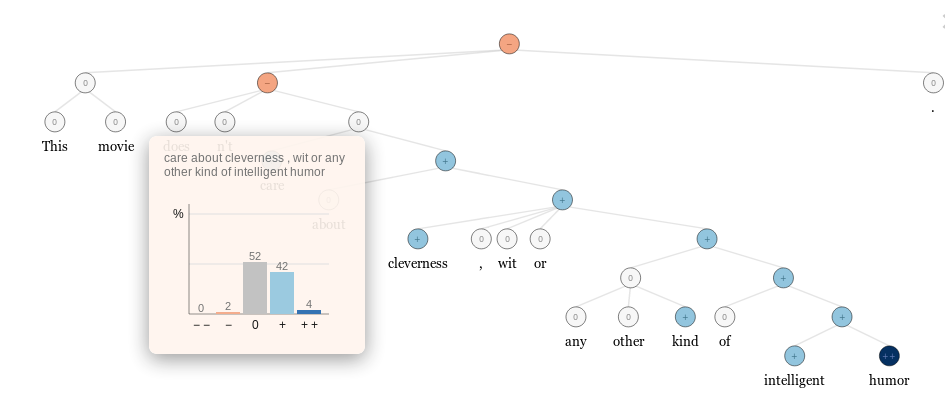
\includegraphics[height=6.5cm]{guide_tree.png}
  \captionof{figure}{Пример результата работы приложения}\label{fig:guide:tree}
\end{center}


% \section{ЭКОНОМИЧЕСКАЯ ЧАСТЬ}
\subsection{Характеристика программного средства}
\subsection{Расчет сметы затрат на разработку и отпускной цены ПО}


% \setcounter{page}{69}
% \subsection{Расчет экономического эффекта у разработчика ПО}
% \setcounter{page}{71}

% \sectioncentered*{Заключение}
\addcontentsline{toc}{section}{ЗАКЛЮЧЕНИЕ}
\label{sec:outro}
В результате выполнения дипломного проекта была разработана система анализа тональностей в тексте. Данное приложение предназначено для сервисов предлагающих товары и услуги множеству пользователей.

Программный продукт возможно адаптировать, для того чтобы автономно собирать информацию о продуктах и услугах, и получать отзывы о них от пользователей. После этого модель нейронной сети позволяет классифицировать данные отзывы по настроениям пользователей. Это помогает выделить какие отзывы требуют внимательного изучения работниками сервиса, а какие из них них не играют большой роли для маркетинга.

Особенностью, которая отличает данное приложение от аналогов, является гибкость системы, и широкие возможности в визуализации результатов анализа. Это достигнуто за счет использования усложненной структуры нейронной сети, что значительно сокращает время ее обучения, и предоставляет пользователю информацию о том, почему модель сделала тот или иной вывод для отзыва. Данная особенность системы дает возможность настроить ее для использования в сервисах, где специфические термины и лексика играют важную роль в семантике отзывов.

Вся собранная и обработанная информация хранится в базе данных, что представляет возможности для регрессионого анализа товаров и услуг.

На основании вышеприведенных сведений, поставленные цели можно считать выполненными в полном объеме. Дальнейшие планы расширения приложения заключаются в увеличении производительности приложения за счет оптимизации оптимизации обработки групп наборов данных. А так же планируется добавление графического интерфеса, что позволит без особых услилий управлять системой.


% Зачем: Изменение надписи для списка литературы
% Почему: Пункт 2.8.1 Требований по оформлению пояснительной записки.
\renewcommand{\bibsection}{\sectioncentered*{СПИСОК ИСПОЛЬЗОВАННЫХ ИСТОЧНИКОВ}}
\phantomsection\pagebreak% исправляет нумерацию в документе и исправляет гиперссылки в pdf
\addcontentsline{toc}{section}{СПИСОК ИСПОЛЬЗОВАННЫХ ИСТОЧНИКОВ}

% Зачем: Печать списка литературы. База данных литературы - файл bibliography_database.bib

\bibliography{bibliography_database}


% \includepdf позволяет включить в результирующий pdf документ часть другого pdf документа, сделанного
% например не с помощью TeX. Бывает полезно, если какие-то диаграммны нарисованы, например, с помощью 
% Microoft Office и сохранены в pdf.
%\includepdf[pages={-}]{documents_list.pdf}

\end{document}